%%%%%%%%%%%%%%%%%%%%%%%%%%%%%%%%%%%%%%%%%%%%%%%%%%%%%%%%%%%%%%%%%%%%%%%%%%%%%%%
%%
%% This file is part of the Home2L project.
%%
%% (C) 2015-2021 Gundolf Kiefer
%%
%% Home2L is free software: you can redistribute it and/or modify
%% it under the terms of the GNU General Public License as published by
%% the Free Software Foundation, either version 3 of the License, or
%% (at your option) any later version.
%%
%% Home2L is distributed in the hope that it will be useful,
%% but WITHOUT ANY WARRANTY; without even the implied warranty of
%% MERCHANTABILITY or FITNESS FOR A PARTICULAR PURPOSE.  See the
%% GNU General Public License for more details.
%%
%% You should have received a copy of the GNU General Public License
%% along with Home2L. If not, see <https://www.gnu.org/licenses/>.
%%
%%%%%%%%%%%%%%%%%%%%%%%%%%%%%%%%%%%%%%%%%%%%%%%%%%%%%%%%%%%%%%%%%%%%%%%%%%%%%%





%%%%%%%%%%%%%%%%%%%%%%%%%%%%% General Header %%%%%%%%%%%%%%%%%%%%%%%%%%%%%%%%%


\documentclass[12pt,english,parskip=half,headheight=19pt]{scrreprt}
\usepackage{scrhack}        % just to avoid "\float@addtolists detected!(scrreprt)" warnings
\usepackage[utf8]{inputenc}
\usepackage[a4paper,tmargin=15mm,bmargin=15mm,lmargin=20mm,rmargin=20mm,includehead,includefoot]{geometry}
\usepackage{lmodern}        % "Latin Modern" font allows italic+bold font
\usepackage[T1]{fontenc}    % see https://tex.stackexchange.com/questions/2369/why-do-the-less-than-symbol-and-the-greater-than-symbol-appear-wrong-as
\usepackage{amssymb}        % for the tutorial $\blacktriangleright$
\usepackage{paralist}       % for \begin{itemize}[...]
\usepackage{longtable}
\usepackage{textcomp}       % for \textdegree
\usepackage{color}

\usepackage{graphicx}       % for .png (non-.svg) images
\usepackage[inkscapelatex=false,keepaspectratio]{svg}

\usepackage{makeidx}       % for index
\usepackage{url}
\usepackage[extension=,colorlinks=true,linkcolor=blue]{hyperref}    % clickable TOC and references with PDFlatex
  % Due to a bug in the LaTeX 'hyperref' package, it appears to be impossible to refer to files or directories
  % without a period in their name. As a workaround, the 'extension' option is set to an empty string here,
  % leading to the affected link targets to end with a period (''.'').
  % A comment in Section~\ref{sec:intro-about} documents this.
\usepackage{listings}
\usepackage{lstautogobble}

%\usepackage[fencedCode=true]{markdown}   % for temporary use

\makeindex


% Suppress "bad box" warnings ...
\hbadness=10000
\hfuzz=\maxdimen
\newcount\hbadness
\newdimen\hfuzz





%%%%%%%%%%%%%%%%%%%%%%%%%%%%% Settings %%%%%%%%%%%%%%%%%%%%%%%%%%%%%%%%%%%%%%%%


% Modes...
\ifdefined\version                                          % 'public' version, for publishing ...
  \newcommand{\figsvg}[2][]{\includesvg[#1]{#2}}            %   Omit references to image file.
\else                                                       % Draft version ...
  \newcommand{\figsvg}[2][]{\href{#2}{\includesvg[#1]{#2}}} %   Create references to image files.
  \newcommand{\version}{Draft}
\fi





%%%%%%%%%%%%%%%%%%% Headings, footers and formatting %%%%%%%%%%%%%%%%%%%%%%%%%%


\usepackage[headsepline,footsepline,plainfootsepline]{scrlayer-scrpage}
\pagestyle{scrheadings}


% Font settings...
\renewcommand{\familydefault}{\sfdefault}
\setkomafont{pageheadfoot}{\textsf}

\automark[chapter]{chapter}

\lohead{\headmark}
\cohead{}
\rohead{\includesvg[height=1.2em]{figs/home2l-icon}}

\lofoot*{\parbox[c][1.4em]{5cm}{The \textit{Home2L} Book}}
\cofoot*{} % \today}
\rofoot*{\thepage}
\renewcommand{\caplabelfont}{\textbf}

%\addtokomafont{section}{\clearpage}
%\addtokomafont{subsection}{\clearpage}

\renewenvironment{description}[1][8ex]
  {\list{}{\labelwidth=5ex \leftmargin=#1 \let\makelabel\descriptionlabel}}
  {\endlist}





%%%%%%%%%%%%%%%%%%%%%%%%%%%%% Listings %%%%%%%%%%%%%%%%%%%%%%%%%%%%%%%%%%%%%%%%


% \code{} for arbitrary code, which is not linked; '_' does not need to be escaped
\DeclareUrlCommand\code{\urlstyle{tt}}

\definecolor{lstbackground}{rgb}{0.9,0.9,0.9}
\definecolor{lstgrey}{rgb}{0.35,0.35,0.35}

\lstdefinelanguage{comments}{
  sensitive=true,
  comment=[l]\#
}

\lstdefinelanguage{bash}{
  sensitive=true,
  comment=[l]\#,
  basicstyle=\ttfamily\footnotesize\color{lstgrey},
  delim=*[l][\color{black}]{\$ },
  moredelim=[il][\color{black}]{§}
}

\lstdefinelanguage{python}{
  sensitive=true,
  comment=[l]\#,
  basicstyle=\ttfamily\footnotesize\color{lstgrey},
  delim=[l][\color{black}]{>>> },
  moredelim=[il][\color{black}]{§}
}

\lstdefinelanguage{home2l}{
  sensitive=true,
  basicstyle=\ttfamily\footnotesize\color{lstgrey},
  delim=[l][\color{black}]{home2l> },
  moredelim=[il][\color{black}]{§}
}

\lstdefinelanguage{brownie2l}{
  sensitive=true,
  basicstyle=\ttfamily\footnotesize\color{lstgrey},
  delim=[l][\color{black}]{brownie2l> },
  moredelim=[il][\color{black}]{§}
}

\lstset{
  basicstyle=\ttfamily\footnotesize,
%  keywordstyle=\bfseries,
%  identifierstyle=,% nothing happens
%  directivestyle=\itshape, % \bfseries,
  commentstyle=\color[rgb]{0.35,0.35,0.35},%\itshape
  backgroundcolor=\color{lstbackground},
  frame=single, %L, % single
  framerule=0pt,
  framesep=5pt,
  xleftmargin=5pt,
  xrightmargin=5pt,
  breaklines=true,
  postbreak=\mbox{\textcolor{red}{$\hookrightarrow$}},  % \space
  prebreak=\mbox{\textcolor{red}{$\hookleftarrow$}},
  autogobble=true,
  columns=fullflexible,  % to make copy-and-paste from the document work
  keepspaces=true,
  showstringspaces=false,
  language={},
  upquote=true
}


\newcommand{\lst}[1]{\colorbox{lstbackground}{\footnotesize\code{#1}}}

\newcommand{\lstf}[1]{\colorbox{lstbackground}{\ttfamily\footnotesize#1}}

\newcommand{\lstbox}[1]{
  \par
  \colorbox{lstbackground}{\ttfamily\footnotesize{\parbox{\linewidth}{#1}}}
  \par
}

%\renewcommand{\lstlistingname}{Listing}






%%%%%%%%%%%%%%%%%%%%%%%%%%%%%%% Info boxes %%%%%%%%%%%%%%%%%%%%%%%%%%%%%%%%%%%%


\newcommand{\infobox}[1]{
  \par
  \medskip
  \hfill
  \setlength\arrayrulewidth{1pt}
  \begin{tabular}[t]{c|c|}
    \parbox{1.8em}{\hfill\textit{\Huge\textbf{i}\,}}
    &
    \,\parbox{0.89\linewidth}{\setlength{\parskip}{0.5em} \small #1}\,
  \end{tabular}
  \medskip
  \par
}


\newcommand{\warnbox}[1]{
  \par
  \medskip
  \hfill
  \setlength\arrayrulewidth{1pt}
  \begin{tabular}[b]{c|c|}
    \includesvg[width=1.8em]{figs/ic-warning}
    &
    \,\parbox{0.89\linewidth}{\setlength{\parskip}{0.5em}#1}\,
  \end{tabular}
  \medskip
  \par
}


\newcommand{\eshockdisclaimer}{
  \warnbox{\textbf{Disclaimer}

    Building electronic circuits requires adequate knowledge in electronics.
    Modifying the electrical installation of a building is inherently dangerous and may result in
    serious damage, injury or even death if not done properly.

    \textit{You expressively agree to hold the authors of the \textit{Home2L} suite and of this
    document harmless for any property damage, personal injury and/or death, or any other loss or
    damage that may result from your use of the information or software provided.}

    This material is provided ''as is''. Use it wisely, it is at your own risk!
  }
}





%%%%%%%%%%%%%%%%%%%%%%%%%%%%% Cross-referencing %%%%%%%%%%%%%%%%%%%%%%%%%%%%%%%


% Defining labels inside this document ...
\newcommand{\labeltool}[1]{\index{#1@\texttt{#1} (tool)} \label{tool:#1}}


% (Internal) Similar labellings for RCs and ENVs are implicitly generated in 'excode.py'...
\newcommand{\labelenv}[1]{\index{#1@\texttt{#1} (configuration)} \label{env:#1}}
\newcommand{\labelrc}[2]{\index{#1@\texttt{#1} (resource driver)!#2@\texttt{#2} (resource)} \label{rc:#2}}


% Defining an arbitrary index entry ...
\newcommand{\idx}[1]{#1\index{#1}}


% References to internal labels ...
\newcommand{\refenv}[1]{\hyperref[env:#1]{\texttt{#1}}}        % add index? last #1 -> '\idx{#1}'
\newcommand{\refrc}[1]{\hyperref[rc:#1]{\texttt{#1}}}
\newcommand{\reftool}[1]{\hyperref[tool:#1]{\texttt{\idx{#1}}}}


% External references (Doxygen, sources tree and world) ...
\newcommand{\refdoc}[2]{\href{#1}{#2}}              % refer to some document inside the source tree
\newcommand{\refsrc}[1]{\href{#1}{\texttt{#1}}}     % refer to some source file

\newcommand{\refapic}[1]{\href{home2l-api_c/index.html}{\mbox{\texttt{#1}}}}            % refer to some C class / function / definition (should be supported by the Doxygen search function)
\newcommand{\refapipython}[1]{\href{home2l-api_python/index.html}{\mbox{\texttt{#1}}}}  % refer to some Python class / function / definition (should be supported by the Doxygen search function)

\newcommand{\refapicgroup}[2]{\href{home2l-api_c/group__#1.html}{#2}}
  % refer to some Doxygen group in the C/C++ API as declarved by '@newgroup'.
  % Note: Underscores must be doubled in the first argument!
\newcommand{\refapipythongroup}[2]{\href{home2l-api_python/group__#1.html}{#2}}
  % refer to some Doxygen group in the Python API as declared by '@newgroup'.
  % Note: Underscores must be doubled in the first argument!

% References to the C/Python API doc in general ...
\newcommand{\theapic}{\refdoc{home2l-api_c/index.html}{C/C++ API}}
\newcommand{\theapipython}{\refdoc{home2l-api_python/index.html}{Python API}}





%%%%%%%%%%%%%%%%%%%%%%%%%%%%%%%%%%%%%%%%%%%%%%%%%%%%%%%%%%%%%%%%%%%%%%%%%%%%%%%
%
%                  Front Matter
%
%%%%%%%%%%%%%%%%%%%%%%%%%%%%%%%%%%%%%%%%%%%%%%%%%%%%%%%%%%%%%%%%%%%%%%%%%%%%%%%


\begin{document}

\sloppy

%\pagenumbering{roman}

\begin{titlepage}
  \centering
  \vfill

  \figsvg[width=5cm]{figs/home2l-icon.svg}
  \vfill

  \scalebox{2.0} {\Huge \textsf{\textbf{The \textit{Home2L} Book}} } \\
  \vskip 2em
  \huge \textsf{\textbf{Smart Tools for a Private Home}}
  \vfill

  \textsf{Gundolf~Kiefer}
  \vfill

  \LARGE Version: \version \\ ~ \\ \today
  \vfill
  \vfill

  \begin{tabular}{rl}  % {|rl|}
    %\hline \rule{0pt}{3ex}
    Jump to: & \hyperref[sec:tutorial-start]{Docker Image and Tutorial} \\
    & \theapic{} \\
    & \theapipython{}
    %\rule[-2ex]{0pt}{0pt} \\ \hline
  \end{tabular}

  \vfill

  \framebox[16cm]{
    \parbox{3cm}{
      \includesvg[width=3cm]{figs/cc-by-sa}
    }
    \hfill
    \parbox{12cm}{\footnotesize This work is licensed under the Creative Commons Attribution-ShareAlike 4.0 International License. To view a copy of this license, visit \url{https://creativecommons.org/licenses/by-sa/4.0} or send a letter to Creative Commons, PO Box 1866, Mountain View, CA 94042, USA.}
  }
\end{titlepage}


\setcounter{secnumdepth}{3}
\setcounter{tocdepth}{3}

\tableofcontents

%\newpage
%\pagenumbering{arabic}




%%%%%%%%%%%%%%%%%%%%%%%%%%%%% Main chapters %%%%%%%%%%%%%%%%%%%%%%%%%%%%%%%%%%


%\part{Overview, Tools and Concepts}



%%%%%%%%%%%%%%%%%%%%%%%%%%%%%%%%%%%%%%%%%%%%%%%%%%%%%%%%%%%%%%%%%%%%%%%%%%%%%%%
%
%
\chapter{Introduction}
\label{ch:intro}
%
%
%%%%%%%%%%%%%%%%%%%%%%%%%%%%%%%%%%%%%%%%%%%%%%%%%%%%%%%%%%%%%%%%%%%%%%%%%%%%%%%



%%%%%%%%%%%%%%%%%%%%%%%%%%%%%%%%%%%%%%%%%%%%%%%%%%%%%%%%%%%%%%%%%%%%%%%%%%
\section{What Are the \textit{Home2Ls}?}
\label{sec:intro-overview}
%%%%%%%%%%%%%%%%%%%%%%%%%%%%%%%%%%%%%%%%%%%%%%%%%%%%%%%%%%%%%%%%%%%%%%%%%%


The \textit{Home2L} \texttt{[houmtu:l]} suite is a collection of tools and libraries for automation in private homes. Its main features and design goals are:


\subsection*{Versatile \textit{Resources} Library}

The central component of the \textit{Home2L} suite is the \textit{Resources} library. It connects physical sensors and actors, software services, computers and more. Everything that can act or sense in the widest sense, can be modelled as a \textit{resource} in the \textit{Home2L} suite.

All \textit{resources} are arranged in a common namespace, but driven and accessed in a completely distribited way from any computer. They can be manipulated or read out using the library, which provides full network transparency and supports arbitrary concurrent accesses from any process on any machine anytime.

Resources are manipulated by means of independent \textit{requests} with individual attributes like priorities and time intervals. The user pushes a button to open the window blinds. One second later, a timer-triggered automatic rule tells the blinds to close. What should happen now? The \textit{request} model allows to clearly specify priorities (e.g. user interaction in favor of automation rules) and to handle concurrency properly.

The \textit{Home2L Shell} is a powerful administration tool and allows to access resources and submit requests on the command line or by shell scripts.

Both automation rules and resource drivers can also be part of a larger program. Any software linking against the \textit{Resources} library can access resources or publish own run-time information as resources.


\subsection*{Efficient and Lightweight Design}

All core components are written in C/C++, with a very minimum set of external dependencies beyond \textit{libc} - ideally suited for small embedded devices and microcontrollers. There is no need for a Java runtime environment or a heavy web framework. Starting up a server and a command shell and shutting both down again takes less than a second altogether - on an ARM-based minicomputer running at 144 MHz!


\subsection*{Ambient Intelligence, No Need for a Central Server}

Central servers are single points of failure. \textit{Home2L} follows a completely distributed concept. Any (mini-)computer can act as part of the network. If resources, such as sensors or actors, are connected to them, they can be exported to any other host in the \textit{Home2L} network. A failure of a host only causes its own resources to be unavailable -- everything else keeps on working.


\subsection*{Automation Rules Written in Python -- But Not Limited to That}

There is no new language or tool to learn to formulate automation rules. \textit{Home2L} rules written in Python profit from the simplicity and power of the Python language. There can be multiple rules scripts, they may run on any machine, and they may be combined with other software routines or be part of larger applications.

Other ways to interact with \textit{Home2L} resources is via the C/C++ API from any application or by shell scripts using the \textit{Home2L Shell} (see Sections~\ref{sec:resources-shell} and \ref{sec:tutorial-shell}).


\subsection*{Integrating Sensors/Actor Hardware and Services: MQTT, Python, Shell Scripts, ...}

MQTT-enabled devices can be imported directly using the MQTT gateway driver (see Sections~\ref{sec:drvlib-mqtt} and \ref{sec:tutorial-mqtt}).

An API for \textit{resource} drivers allows to easily add support for new hardware or software services. A driver can be implemented in C/C++, in Python, or as a shell script. For all these cases, documented examples can be found in the source tree (see Section~\ref{sec:resources-drvdev}).


\subsection*{Easy Integration of ''Do-it-Yourself'' Hardware}

\textit{Home2L Brownies} are programmed low-cost microcontrollers (\textit{AVR ATtiny 84/85/861}) connected to a Linux host over 4-wire cables (e.g. KNX/EIB cables). The bus protocol is based on \textit{i2c}, robust and allows to build very simple, self-made hardware nodes. Just an \textit{ATtiny} device and two resistors are enough to build a sensor node! Details can be found in Chapter~\ref{ch:brownies} and Section~\ref{sec:tutorial-brownies}.


\subsection*{Privacy}

The \textit{Home2Ls} do not need an Internet connection and do not try to communicate with hosts other than they are configured to. By design, the \textit{Home2Ls} communicate with each other over a (trusted) LAN, which can easily be set up and secured using standard Linux/UNIX techniques. The open source licensing ensures transparency for what the software does inside the user's private home.


\subsection*{Modularity}

The core part, the \textit{Resources} library, is kept small and portable with APIs for application programs and drivers in C/C++ and Python. All other components are optional and can be used or replaced by alternatives as desired by the user.

Figure~\ref{fig:home2l-components} shows an overview on the \textit{Home2L} suite. It contains a collection of mutually independent applications (blue). The central component is the \textit{Home2L Resources} library, which is used by all applications. Resource drivers (brown) are also optional and provide interfaces to sensors, actors or services like \textit{MQTT} brokers.

\begin{figure}[ht]
  \centering
  \figsvg[width=0.9\linewidth]{figs/home2l-components.svg}
  \caption[l]{\textit{Home2L} Components:
    \textcolor[rgb]{0.2,0.3,1.0}{Tools},
    \textcolor[rgb]{0.5,0.25,0}{Drivers},
    \textcolor[rgb]{0,0.5,0}{Libraries}
  }
  \label{fig:home2l-components}
\end{figure}



%%%%%%%%%%%%%%%%%%%%%%%%%%%%%%%%%%%%%%%%%%%%%%%%%%%%%%%%%%%%%%%%%%%%%%%%%%
\clearpage
\section{About This Book}
\label{sec:intro-about}
%%%%%%%%%%%%%%%%%%%%%%%%%%%%%%%%%%%%%%%%%%%%%%%%%%%%%%%%%%%%%%%%%%%%%%%%%%

This book serves as the main user and reference manual for the \textit{Home2L} suite.

Further information can be found in the \theapic{} and the \theapipython{} documentation.
Consulting the API documentation is particularly helpful for writing own resource drivers,
sophisticated automation rules or applications using some \textit{Home2L} library.

Presently, the \textit{Home2L Book} is still under construction and primarily targets readers
with computer skills. Not all existing features are already documented in this book.
Extending the book to provide good end-user documentation is subject to future work
(see Section~\ref{sec:helping}).

The \textit{Home2L} suite comes with a \hyperref[sec:tutorial-start]{Docker Demo Image}. Chapter~\ref{ch:tutorial} contains a step-by-step tutorial based on this image demonstrating the core concepts and features of the \textit{Home2L} suite. This should be the starting point for any new user.

Chapters~\ref{ch:installing} and ~\ref{ch:managing} cover the installation and administration of a \textit{Home2L} cluster.

Chapter~\ref{ch:resources} explains the concepts and usage of the \textit{Resources} library, the core component of the \textit{Home2L} suite. This is followed by explanations on how to write automation rules in Chapter~\ref{ch:rules}.

Chapter~\ref{ch:brownies} introduces the \textit{Brownies} subproject. This includes a description of the physical properties and the protocol of the \textit{Brownie} automation bus, an introduction to the software stack on the microcontroller and on the Linux host side, as well as example circuits.

The following chapters cover the main user applications, presently the \textit{Home2L WallClock} (Chapter~\ref{ch:wallclock}) and the \textit{Home2L DoorMan} (Chapter~\ref{ch:doorman}).

Chapter~\ref{ch:drvlib} documents the library of drivers supplied with the \textit{Home2L} base distribution.


\infobox{
  \textbf{Links in this document}

  This document makes extensive use of links pointing into the code documentation or the source tree to help finding
  relevant information quickly. Some hints on using these links:
  \begin{itemize}
    \item
      Some links name a code object in the text (e.g. a function, class or macro), and the links refer to the root
      of the \theapic{} or the \theapipython{} documentation. In such a case, you can usually copy the name of the code object
      and paste it into the ''search'' field of the code documentation web page to quickly navigate to the respective code.
    \item
      Some links point to some file or directory in the source tree. Due to a bug in the LaTeX ''hyperref'' package,
      it appears to be impossible to refer to a file or directory without a period in its name.
      As a workaround, some link targets end with an extra period (''.'').
      Please remove an eventual trailing period if it occurs in a link target.
  \end{itemize}
}



%%%%%%%%%%%%%%%%%%%%%%%%%%%%%%%%%%%%%%%%%%%%%%%%%%%%%%%%%%%%%%%%%%%%%%%%%%
\clearpage
\section{How Can I Help?}
\label{sec:helping}
%%%%%%%%%%%%%%%%%%%%%%%%%%%%%%%%%%%%%%%%%%%%%%%%%%%%%%%%%%%%%%%%%%%%%%%%%%


The project has been published with the hope that is useful to the community.
To let the project grow further and make available to a wider audience,
volunteers and partners are needed and welcome.

Great contributions are:

\begin{enumerate}

  \item \textbf{Report and help fixing bugs.}

  \item Make \textbf{sample installations}, document them and share your experiences.

  \item \textbf{Packaging}: Create packages for major Linux distributions.

  \item \textbf{Documentation}: Write good documentation, particularly for end users.

\end{enumerate}

For any questions on how to participate, do not hesitate to contact us
via the project page.



%%%%%%%%%%%%%%%%%%%%%%%%%%%%%%%%%%%%%%%%%%%%%%%%%%%%%%%%%%%%%%%%%%%%%%%%%%
\section{Questions?}
\label{sec:support}
%%%%%%%%%%%%%%%%%%%%%%%%%%%%%%%%%%%%%%%%%%%%%%%%%%%%%%%%%%%%%%%%%%%%%%%%%%


Feel free to drop a mail to: \lstf{Gundolf Kiefer <gundolf.kiefer@web.de>}





%%%%%%%%%%%%%%%%%%%%%%%%%%%%%%%%%%%%%%%%%%%%%%%%%%%%%%%%%%%%%%%%%%%%%%%%%%%%%%%
%
%
\chapter{Tutorial: Have a Test Drive!}
\label{ch:tutorial}
%
%
%%%%%%%%%%%%%%%%%%%%%%%%%%%%%%%%%%%%%%%%%%%%%%%%%%%%%%%%%%%%%%%%%%%%%%%%%%%%%%%





%%%%%%%%%%%%%%%%%%%%%%%%%%%%%%%%%%%%%%%%%%%%%%%%%%%%%%%%%%%%%%%%%%%%%%%%%%
\section{Introduction}
\label{sec:tutorial-intro}
%%%%%%%%%%%%%%%%%%%%%%%%%%%%%%%%%%%%%%%%%%%%%%%%%%%%%%%%%%%%%%%%%%%%%%%%%%


\subsection{Overview}

This step-by-step tutorial aims to give an introduction to the \textit{Home2L} suite covering all core tools and concepts of the suite. It should be the starting point for anybody new to the software.

This tutorial will introduce you to:

\begin{itemize}
  \item the main \textit{Home2L} concepts and capabilities.

  \item \textit{Home2L Resources}: values and states, subscriptions, requests, the directory.

  \item the \textit{Home2L Shell} for inspection, maintenance, and logging.

  \item the MQTT gateway.

  \item \textit{Home2L Brownies} and the integration of do-it-yourself hardware.

  \item the \textit{WallClock} information display and UI.

  \item writing automation rules using the \theapipython{}.

  \item several command line tools: \reftool{home2l-shell}, \reftool{home2l-wallclock}, \reftool{home2l-daemon},
      \reftool{home2l-server}, \reftool{home2l-brownie2l}.

  \item many code examples for automation rules and drivers.

\end{itemize}

The tutorial can be performed using a prepared Docker container image with a complete showcase demo setup. No manual installation is necessary.

Sections~\ref{sec:tutorial-start} -- \ref{sec:tutorial-shell} introduce the showcase system and basic concepts of the \textit{Home2L} suite. The remaining subsections cover dedicated topics and can be exercised independently from each other, depending on your interests and preferences.



\subsection{Prerequisites}

To run the tutorial you need

\begin{itemize}
  \item \href{https://en.wikipedia.org/wiki/Docker_(software)}{Docker (Version 18.09.01 or above)},
  \item a host system with a running X11 server (e.~g. an arbitrary Linux distribution).
\end{itemize}

Alternative ways of running the tutorial without the supplied Docker image are described in Section~\ref{sec:tutorial-nodocker}.



\subsection{Notational Conventions}

The tutorial uses the following conventions in notation:

\begin{enumerate}[a)]
  \item A black triangle ($\blacktriangleright$) marks an instruction to follow.
  \item \lstf{Typewriter text with a grey background} marks an interaction with your computer.
    Lines starting with a prompt indicate commands to be entered into the respective
    interpreter:
    \begin{description}
      \item[\lstf{\$}] -- the Linux shell (\textit{bash}),
      \item[\lst{home2l>}] -- the \textit{Home2L Shell},
      \item[\lst{>>>}] -- the Python command interpreter.
    \end{description}
\end{enumerate}


\subsubsection*{Example}

\begin{itemize}[$\blacktriangleright$]
  \item Enter the following commands to verify your computer's calculation skills:
    \begin{lstlisting}
    $ python3
    >>> 2+3
    5
    \end{lstlisting}
    Then push \textit{Ctrl-D} to quit the Python shell again.
\end{itemize}


\subsubsection*{Info and Warning Boxes}

\infobox{
  Info boxes contain some additional information, not essential to just run the tutorial successfully.
}

\warnbox{
  Warning boxes contain important information. You should read it, otherwise the tutorial may not work
  as expected, or some other kind of problem may occur.
}





%%%%%%%%%%%%%%%%%%%%%%%%%%%%%%%%%%%%%%%%%%%%%%%%%%%%%%%%%%%%%%%%%%%%%%%%%%
\clearpage
\section{Starting the Showcase Environment}
\label{sec:tutorial-start}
%%%%%%%%%%%%%%%%%%%%%%%%%%%%%%%%%%%%%%%%%%%%%%%%%%%%%%%%%%%%%%%%%%%%%%%%%%


\begin{itemize}[$\blacktriangleright$]

\item
  On your host PC, open a terminal window and enter:
  \begin{lstlisting}[language=bash]
  $ xhost +local:        # allow X11 applications in the container to open windows
  $ docker run -ti --rm --name home2l-showcase --hostname home2l-showcase \
  §    -e DISPLAY=$DISPLAY -v /tmp/.X11-unix:/tmp/.X11-unix --device /dev/snd \
  §    gkiefer/home2l
  \end{lstlisting}

\end{itemize}

\textbf{That's it!}

You should now have two windows open as shown in Figure~\ref{fig:tutorial-start}. The left window is your original terminal window, in which the \textit{ShowHouse} console tool is running (\reftool{home2l-showhouse}). It simulates the house and the physical world. The right window shows a \textit{WallClock}instance (\reftool{home2l-wallclock}), which simulates a virtual tablet computer mounted at the living room wall of your virtual home.

\begin{figure}[ht]
  \centering
  \figsvg[width=0.95\linewidth,keepaspectratio]{figs/tutorial-start.svg}
  \caption[l]{Open windows after starting the showcase environment}
  \label{fig:tutorial-start}
\end{figure}

\begin{itemize}[$\blacktriangleright$]
\item
  (Recommendation) On your host PC, add the following lines to your \lstf{.bashrc} file:
  \begin{lstlisting}[language=bash]
  $ alias DOCKER="docker exec -ti home2l-showcase"
  $ alias DOCKER_ROOT="docker exec -ti --user=root home2l-showcase"
  \end{lstlisting}
  The Docker container is running several foreground and background processes (to be explored later).
  In future steps, you may want or need to start additional programs inside the running container.
  These aliases facilitate starting shells and tools inside the container.
\end{itemize}

\infobox{
  Example invocations are:
  \lstbox{
    \begin{tabular}{ll}
    \$ DOCKER bash            & \# Run a (Unix) shell \\
    \$ DOCKER home2l shell    & \# Run \reftool{home2l-shell} \\
    \$ DOCKER\_ROOT bash      & \# Run a root shell
    \end{tabular}
  }
  Of course, these actions can also be performed without modifying your personal \lstf{.bashrc} file:
  \lstbox{
    \begin{tabular}{ll}
    \$ docker exec -ti home2l-showcase bash            & \# Run a (Unix) shell \\
    \$ docker exec -ti home2l-showcase home2l shell    & \# Run \reftool{home2l-shell} \\
    \$ docker exec -ti {-}{-}user=root home2l-showcase bash      & \# Run a root shell
    \end{tabular}
  }
}





%%%%%%%%%%%%%%%%%%%%%%%%%%%%%%%%%%%%%%%%%%%%%%%%%%%%%%%%%%%%%%%%%%%%%%%%%%
\clearpage
\section{Exploring the Show House}
\label{sec:tutorial-firststeps}
\labeltool{home2l-showhouse}
%%%%%%%%%%%%%%%%%%%%%%%%%%%%%%%%%%%%%%%%%%%%%%%%%%%%%%%%%%%%%%%%%%%%%%%%%%


Now that the \textit{Home2L} showcase environment is up and running, it is time to enter the virtual show house and look around a little bit.

Purpose of this section is to
\begin{itemize}
  \item give an overview on the showcase system,
  \item introduce basic \textit{Home2L} features from a user perspective,
  \item demonstrate the distributed design paradigm and failure tolerance of the \textit{Home2Ls},
  \item give a first impression of the capabilities of the \textit{Resources} library.
\end{itemize}


\subsection{Overview}
\label{sec:tutorial-firststeps-overview}

The \textit{Home2L} suite follows a highly distributed design paradigm. At this point, there are 4 \textit{Home2L instances} running on your machine -- two are visible, two others are running in the background:

\begin{enumerate}

  \item
    The \textit{ShowHouse} Console Tool (\reftool{home2l-showhouse}, left in Figure~\ref{fig:tutorial-start}) is a simulator for the
    physical world of the demo system. This little console application contains a \textit{Resource} driver providing a
    simulated motion sensor, a door lock sensor, window shades, a door light and some other gadgets. The user (you) can
    simulate physical actions by key presses, and some gadgets are visualized in the ASCII art picture.

  \item
    The \textit{WallClock} (\reftool{home2l-wallclock}, right in Figure~\ref{fig:tutorial-start}) is a universal
    information display to be mounted on room walls or installed on mobile devices. This instance is (virtually)
    mounted in the living room of the (virtual) house.

  \item
    A \reftool{home2l-server} instance is running in the background, which in this tutorial hosts the weather driver
    (\reftool{home2l-drv-weather}) and the MQTT gateway (\reftool{home2l-drv-mqtt}).

  \item
    A background script (\reftool{rules-showhouse}) executes various automation rules, for example to close the shades
    at night or to automate the outdoor light. This script will be explored later in Section \ref{sec:tutorial-rules}.

\end{enumerate}

The following subsections explore this setup step by step, beginning with the most visible instances.

\infobox{
  \textbf{There is no central server! The \textit{Home2Ls} do not need one.}

  Even if there is an instance \reftool{home2l-server} whose name suggests so,
  a \textit{Home2L} installation does not need a central server.
  In this example, the weather and the MQTT drivers could as well be loaded and executed by \textit{any}
  of the other three \textit{Home2L} instances.

  In a larger installation, it may be useful to run multiple
  \textit{Home2L} server instances in order to improve failure resilience,
  to attach sensors/actors to different machines, or for maintenance reasons.

  The assignment of the drivers to the \textit{server} instance is
  configured in the \reftool{home2l.conf} configuration file and may be changed there.
}


\subsection{The \textit{WallClock} Main Screen}
\label{sec:tutorial-firststeps-wallclock}

The \textit{WallClock} display shows the current time and date in its upper area. The bottom row contains launcher buttons to access the integrated calendar and music applets (to be explored later).

\infobox{
  \textbf{Resizing the \textit{WallClock} window}

  The \textit{WallClock} window can be resized arbitrarily, and the UI is scaled automatically
  to fit into the window. Alternatively, the window can quickly be resized to
  reasonable sizes by pushing \textit{F9} (half size), \textit{F10} (normal) and
  \textit{F11} (fullscreen), respectively. By pushing \textit{F12}, the size can be fixed
  (may be useful when using a tiling window manager like \textit{awesome}).

  For the tutorial, it is best to keep it in its normal size (\textit{F10}).
}

In the lower part of the display between the date and the launcher buttons, the values of several sensors are visualized. These are, from left to right:

\begin{enumerate}
  \item the local outside temperature,
  \item the \textit{radar eye} -- a visualization of weather radar data around the building
    (the location is pre-configured for Augsburg, Germany),
  \item the mini floor plan,
  \item the room temperature.
\end{enumerate}

Each of these fields visualizes some or multiple \textit{Home2L Resources} provided by different sources.

\infobox{
  \textbf{If the outside temperature or radar eye are missing ...}

  ... don't worry!

  The weather driver depends on an available internet connection and on the \textit{OpenData} server of
  the German Weather Service (DWD). If the server is not reachable this time, the weather-related items
  are missing in the \textit{WallClock} display.
  If so: Do not worry, the other parts of the tutorial are not affected.

  You can diagnose the availabilty of weather data by running the weather driver directly
  in a terminal:
  \lstbox{
    \$ DOCKER bash \\
    \$ .~/opt/home2l/env.sh \\
    \$ /opt/home2l/lib/home2l-drv-weather weather.debug=1
  }
}



\subsection{The \textit{WallClock} Floor Plan}
\label{sec:tutorial-firststeps-floorplan}

By pushing (or clicking on) the mini floor plan, you can open the full floor plan view (see Figure~\ref{fig:tutorial-floorplan}). The buttons on the bottom of the display are mainly used to set the presence (use) state of the user (from left to right):

\begin{enumerate}
  \item ''Back'' button to return to the home screen,
  \item ''Auto'' button to let the presence state be set automatically based on the daytime.
  \item User is at home at day time.
  \item User is at home and sleeping.
  \item User is away temporarily (e.g. for work).
  \item User is away for longer (e.g. on vacation).
\end{enumerate}

The currently active use state is indicated with a yellow label.

Depending on the use state, certain elements of the floor plan are highlighted. For example, the user is reminded to close the windows when leaving home or to lock the door over night.

\begin{figure}[ht]
  \centering
  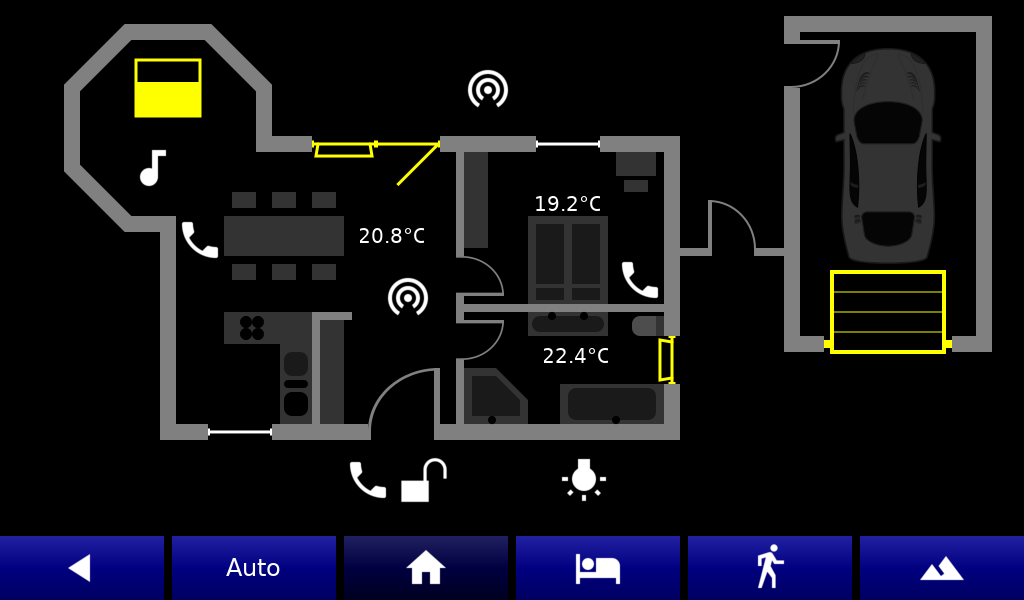
\includegraphics[width=0.7\linewidth]{figs/wallclock-floorplan-3.png}
  \caption[l]{The \textit{WallClock} floor plan}
  \label{fig:tutorial-floorplan}
\end{figure}



\subsection{The \textit{ShowHouse} Console Tool}
\label{sec:tutorial-firststeps-showhouse}

The \textit{ShowHouse} console tool allows to simulate certain physical user actions and weather events.

\begin{itemize}[$\blacktriangleright$]

  \item
    In the \textit{WallClock} window, push (or click on) the mini floor plan to open the full floor
    plan view.

    Then focus the \textit{ShowHouse} window.

  \item
    Press the keys listed in the \textit{ShowHouse} window and see how the various gadgets
    (daylight, door lock status, motion, ...) are visualized in the ASCII art and in the floor plan.

    Did you notice that ...
    \begin{itemize}
      \item the shades close automatically at night?
      \item the door light is activated for a few seconds if motion is detected (press ''M''),
        but only at night time?
      \item at night time, open windows or an unlocked main door are highlighted to draw the
        user's attention to it?
      \item during rainy weather, the \textit{WallClock} excitedly reminds you to close open windows?
    \end{itemize}

    The first two points are controlled by the rules script discussed later in
    Section~\ref{sec:tutorial-rules}.

  \item
    In the \textit{WallClock} window, return to the home screen (push the ''back'' button).
    Then repeat the previous step to see that most gadgets are also visible in the
    mini floor plan.

    What happens, if it starts to rain while a window is open?

\end{itemize}


\subsection{Controlling the Home with the \textit{WallClock}}
\label{sec:tutorial-firststeps-dialogs}

The \textit{WallClock} floor plan view allows to view, but also to interactively control various
gadgets in the house. Since the gadgets are represented by \textit{Home2L} resources
(see Chapter~\ref{ch:resources}), some more sophisticated controls are possible compared to other
home automation user interfaces. For example, the user can override an automation rule for a given time
and let the rule dominate again afterwards. Request attributes (see Section~\ref{sec:tutorial-shell-manipulate}
and Section~\ref{sec:resources-requests}) can be set in order to, for example, not just turn on a light now,
but to autmatically turn it off again in an hour.


\subsubsection{Everyday Use}

Simple switching lights or closing shades is almost as easy as pushing a light button.
Especially for household members with little technical affinity, it is important that standard use cases are easy.

\begin{itemize}[$\blacktriangleright$]

  \item
    In the \textit{WallClock} window, switch to the floor plan screen. In the \textit{ShowHouse} window,
    make sure that it is day time and the weather is good (no rain).

  \item
    Long-push on the light icon near the main door and see that the light turns on.
    Long-push again and see that the light turns off again.

  \item
    Long-push on the kitchen window shades (highlighted in Figure~\ref{fig:tutorial-floorplan-shades}) and
    see that the shades move down and -- after another long push -- up again.

    \begin{figure}[ht]
      \centering
      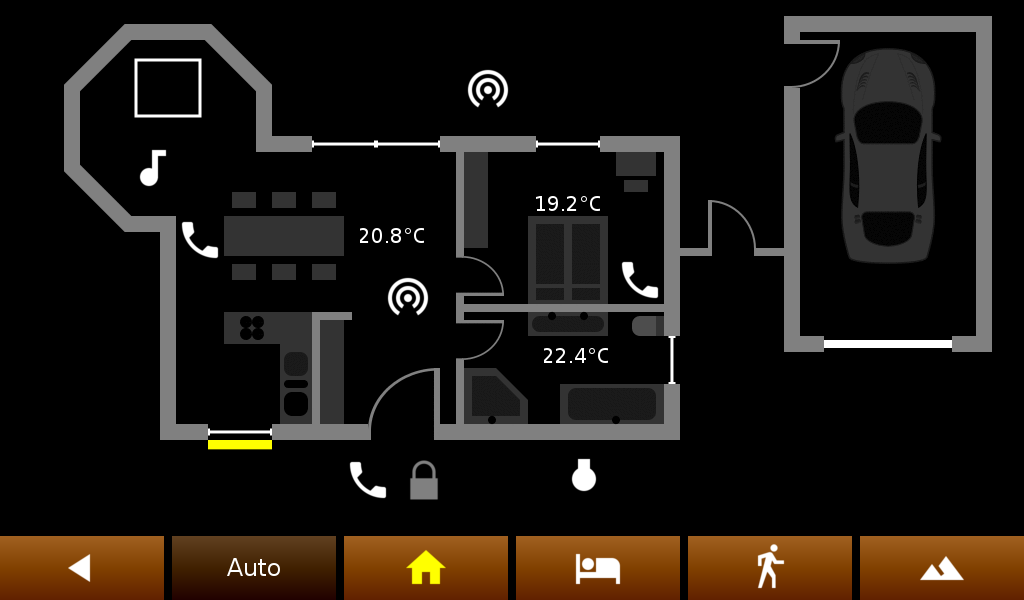
\includegraphics[width=0.65\linewidth]{figs/wallclock-floorplan-shades.png}
      \caption[l]{Floor plan with the kitchen shades partially closed (yellow)}
      \label{fig:tutorial-floorplan-shades}
    \end{figure}

  \item
    Click on one of the WiFi icons to switch on the (virtual) WiFi access points.

  \item
    Open some windows and unlock the main door by pushing the respective buttons in the
    \textit{ShowHouse} window.

    Now assume, you have to leave the house for a short (or a longer) period of time.
    Click on the ''temporarily away'' (or ''away for longer'') button in the bottom right
    of the screen. See how the system reminds you to close the windows and eventually
    switch off the access points before you leave!

    Finally, click on the ''Auto'' button to indicate that you are back home.

\end{itemize}



\subsubsection{The Resource Dialog}

Sometimes, just toggling between ''on'' and ''off'' or ''fully up'' and ''fully down'' is not sufficient,
and a more fine-grained control is desired.
Also, it is not always obvious how the above interactions interfere with the automation rules (remember that
both the door light and the shades are also subject to automation). This is, where \textit{resource dialogs} come into play.

\begin{itemize}[$\blacktriangleright$]

  \item
    Tap on the light icon near the main door. The \textit{resource dialog} shown in
    Figure~\ref{fig:tutorial-floorplan-light} appears.

    \begin{figure}[ht]
      \centering
      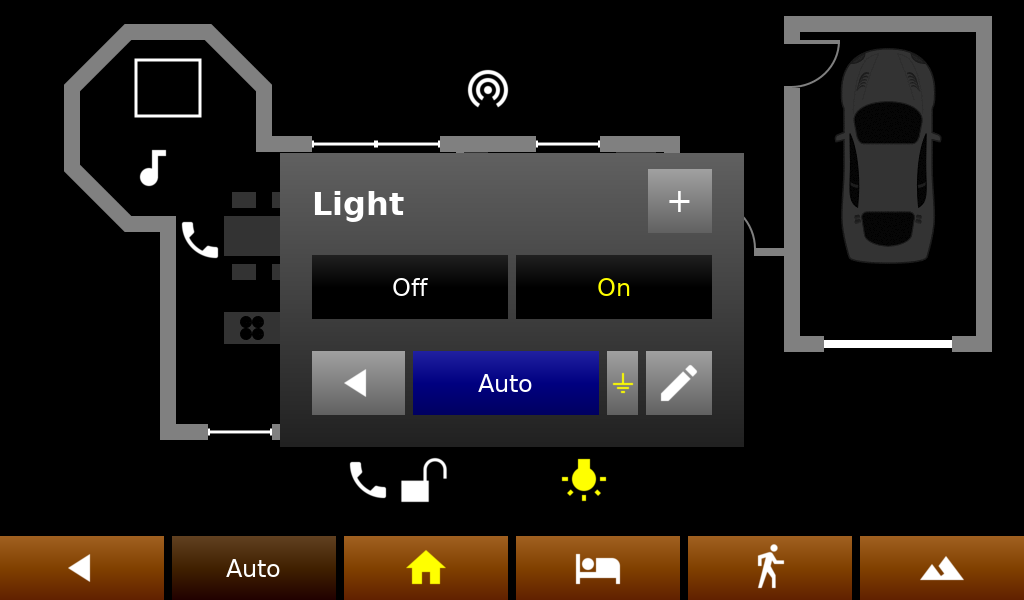
\includegraphics[width=0.65\linewidth]{figs/wallclock-floorplan-light.png}
      \caption[l]{Resource dialog (door light)}
      \label{fig:tutorial-floorplan-light}
    \end{figure}

    \infobox{
      The dialog basically offers three options / buttons: ''Off'', ''On'', and ''Auto''.
      The first two issue a request to turn the light off or on, respectively. The ''Auto'' button
      removes the current user requests. Usually, automation rules take over control then.
    }

  \item
    Select ''Off'', ''On'', and ''Auto''. See how the light behaves in each case.
    Also push ''D'' and ''M'' in the \textit{ShowHouse} window and see that the automation
    rule for turning on the light at night on motion is only effective if ''Auto'' has
    been selected in the resource dialog.
    \infobox{
      Usually, the dialog disappears after pushing one of the value or ''Auto'' buttons.
      By pushing long on these buttons, the dialog stays open.
    }
    \infobox{
      Two values are relevant for a resource, which are often -- but not always -- the same:
      \begin{enumerate}[a)]
        \item the real value,
        \item the desired value as requested by the user.
      \end{enumerate}
      By convention, the real value is shown in yellow color, and the currently requested value
      is indicated by a colored (blue, in this example) button.
    }
    Finally, select ''Auto'' again and close the dialog.

  \item
    Tap on the kitchen window shades. A \textit{resource dialog} similar to the one shown in
    Figure~\ref{fig:tutorial-floorplan-shades-auto} appears.

    \begin{figure}[ht]
      \centering
      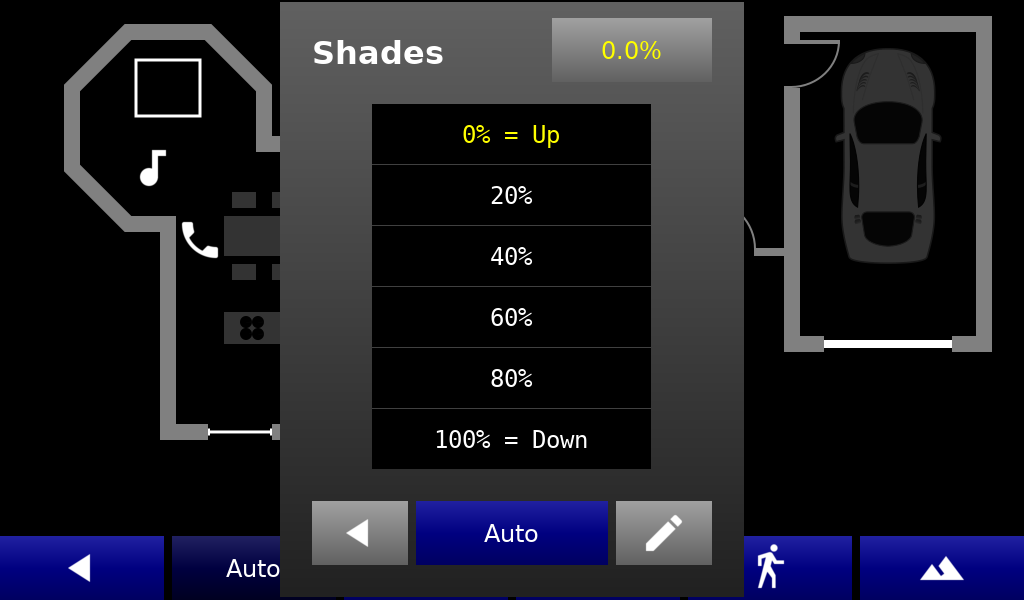
\includegraphics[width=0.65\linewidth]{figs/wallclock-floorplan-shades-auto.png}
      \caption[l]{Resource dialog for shades (no user request)}
      \label{fig:tutorial-floorplan-shades-auto}
    \end{figure}

  \item
    Close the shades by pushing the ''100\%'' button and open them again by selecting
    ''0\%''. You may also close them partially by pushing any other numbered button
    (see Figure~\ref{fig:tutorial-floorplan-shades-user}).

    \begin{figure}[ht]
      \centering
      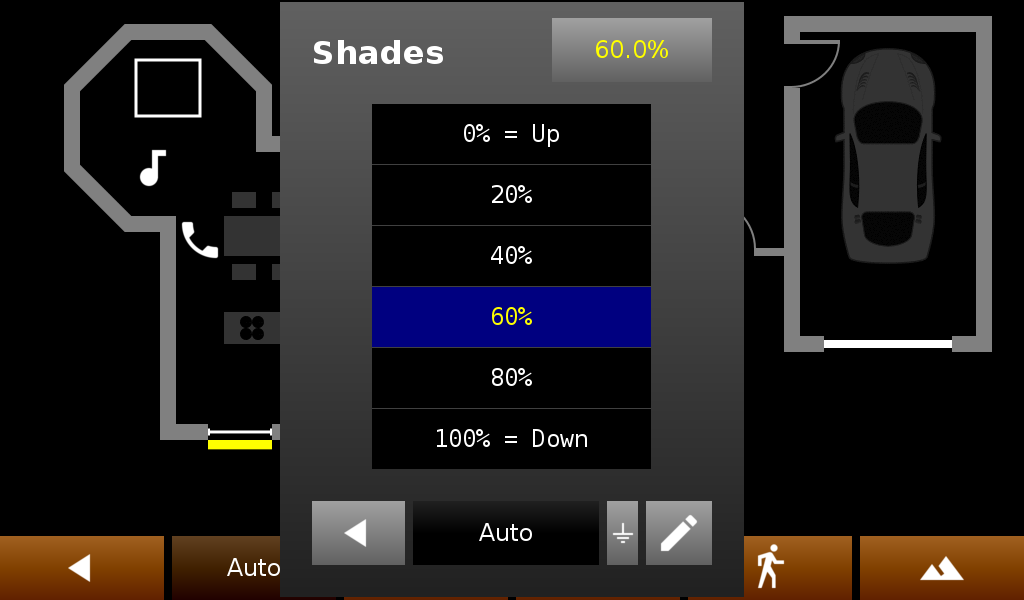
\includegraphics[width=0.65\linewidth]{figs/wallclock-floorplan-shades-user.png}
      \caption[l]{Resource dialog for shades (60\% position)}
      \label{fig:tutorial-floorplan-shades-user}
    \end{figure}

  \item Press ''D'' in  the \textit{ShowHouse} window to toggle between day and night and
    see that the kitchen shades no longer close at night. This is because the user (you) has set a
    manual request in the previous step, and this user request has higher priority than the
    automation rule.

  \item
    Select ''Auto'' in the resource dialog. Then press ''D'' in the \textit{ShowHouse} window to
    toggle between day and night and see that the kitchen shades automatically close at night
    and open at day time again.

  \item
    Tap on other gadgets in the floor plan and see how you can manipulate them.
    \infobox{
      The roof window has two controllable actuators: one for electrical shades, one for a window opener.
      A short tap opens the resource dialog for the shades. A long push opens the dialog for the
      window opener (with red buttons for disambiguation).
    }

\end{itemize}


\subsubsection{Advanced Usage}

The effects demonstrated above are implemented by the \textit{Resource} library and its models.
Sometimes, the standard dialog cannot show the whole truth in all detail. For example, automation rules
for safety-critical actions may place requests with a higher priority than normal user requests, and
the user may wonder why his interaction appears to have no effect.

This section shows how to look ''under the hood'' and to inspect all details of a resource.

\begin{itemize}[$\blacktriangleright$]

  \item
    Open the resource dialog (Figure~\ref{fig:tutorial-floorplan-shades-auto}) for the kitchen window shades,
    and push the button on the upper right (showing ''0.0\%'' in the figure). The dialog expands as
    shown in Figure~\ref{fig:tutorial-floorplan-shades-details}.

    \begin{figure}[ht]
      \centering
      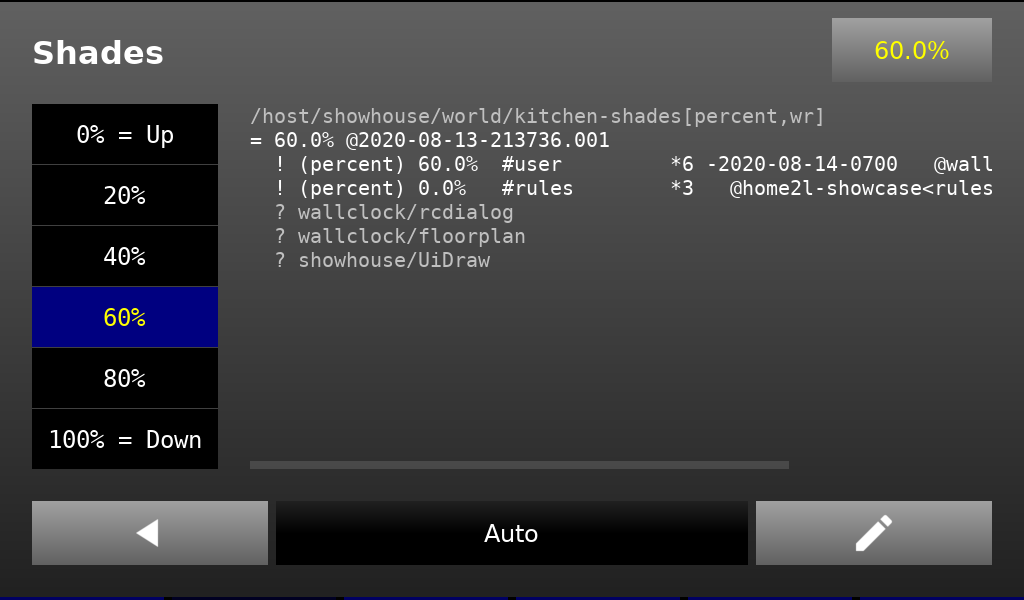
\includegraphics[width=0.7\linewidth]{figs/wallclock-floorplan-shades-details.png}
      \caption[l]{Resource dialog with details}
      \label{fig:tutorial-floorplan-shades-details}
    \end{figure}

    The text display is the raw representation of the underlying resource (details will follow in
    Section~\ref{sec:tutorial-shell-inspect}).
    \begin{itemize}
      \item The first line shows the resource ID and type information.
      \item The second line shows the current value.
      \item Lines starting with ''!'' represent pending requests. The request labeled \lst{#user}
        represents the current user request, the request \lst{#rules} has been set by the
        automation script. In the example, the user request has a priority of 6 (\lst{*6}), the
        rules request has a lower priority of 3 (\lst{*3}).
    \end{itemize}

  \item
    Push various value buttons (0\%, ..., 100\%) or the ''Auto'' button and see how
    the \lst{#user} request changes or disappears and how the actual value changes.
    \infobox{
      The edit button (bottom right) of the resource dialog allows to edit the request attributes
      of the user request. For example, a start and/or end time or an alternative priority can be defined.
      Also, values for which no button exists (e.g. odd percentage numbers) can be set here.

      The syntax for request attributes is described in Section~\ref{sec:resources-syntax}.
      The request ID (\lst{#user}) cannot be changed.
    }

  \item
    Finally, push ''Auto'' and close the kitchen shades dialog again.

  \item
    Long-push on the roof window, expand the window dialog and open the roof window (100\%).
    Then press ''R'' in the \textit{ShowHouse} window to simulate bad weather.
    See how the window is closed during rain to avoid damage in the house, the request \lst{#safety}
    has a higher priority than the user request.
    \infobox{
      The request \lst{#safety_wd} is a watchdog request to additionally increase the reliability
      and enforce a fail-safe behavior if the automation rule or some network connection fails.
      Details are explained in the \reftool{rules-showhouse} file.
    }

\end{itemize}



\subsection{Is All This Stable and Robust? -- Failure Resilience}
\label{sec:tutorial-firststeps-robust}

The following steps examine how the system behaves if one or several \textit{Home2L} instances fail. Failure handling and reporting is provided by the \textit{Resources} library to facilitate application development.

\begin{itemize}[$\blacktriangleright$]

  \item
    In the \textit{WallClock} window, switch back to the home screen.
    Then focus the \textit{ShowHouse} window.

  \item
    Quit the \textit{ShowHouse} (press ''Q'') and see the mini floor plan and the room temperature
    disappearing in the \textit{WallClock} display. These resources were (mainly) provided
    by the \textit{ShowHouse} process, which is now no longer running.

  \item
    Stop the background processes (\reftool{home2l-server} and \reftool{rules-showhouse}) by entering:
    \begin{lstlisting}[language=bash]
    $ home2l demo stop
    \end{lstlisting}
    The weather information displays disappears, and the automation rules stop working.

  \item
    Start the \textit{ShowHouse} again:
    \begin{lstlisting}[language=bash]
    $ home2l showhouse
    \end{lstlisting}
    The floor plan and the inside temperature appear again.

    Toggle between day and nighttime (press ''D'') and simulate motion at night (press ''M'').
    The light is not turned on and the shades do not close at night, because the automation rules
    script is not working!

  \item
    Finally, quit the \textit{ShowHouse} (press ''Q'') and start everything again:
    \begin{lstlisting}[language=bash]
    $ home2l demo start
    $ home2l showhouse
    \end{lstlisting}

\end{itemize}

In summary, these examples show that whenever a \textit{Home2L} instance fails, only the resources or functionalities of failing instance stop working. Everything else remains available. There is no single point of failure. By the remaining tools, the absence of a resource is detected reliably, in many cases instantaneously.





%%%%%%%%%%%%%%%%%%%%%%%%%%%%%%%%%%%%%%%%%%%%%%%%%%%%%%%%%%%%%%%%%%%%%%%%%%
\clearpage
\section{Using the \textit{Home2L Shell}: Behind the Scenes}
\label{sec:tutorial-shell}
%%%%%%%%%%%%%%%%%%%%%%%%%%%%%%%%%%%%%%%%%%%%%%%%%%%%%%%%%%%%%%%%%%%%%%%%%%


The \textit{Home2L Shell} (\reftool{home2l-shell}) is the command line interface to the \textit{Resources} library and serves as a ''swiss army knife'' to access and inspect the resources and servers of a \textit{Home2L} cluster. With the \textit{Home2L Shell} you can inspect all servers and list and inspect all resources. Furthermore, it can be used in a batch mode in a very flexible way for tasks like data logging, manipulating resources from shell scripts or for testing new drivers.

This section gives an introduction to the \textit{Home2L Shell}, which we will use to take a look behind the scenes of the \textit{ShowHouse}. In particular, we will use the shell to check the status of all \textit{Home2L} instances, explore the directory tree, manipulate and monitor resources, and use the \textit{Home2L Shell} for data logging.





%%%%%%%%%%%%%%%%%%%%%%%%%%%%%%%%%%%%%%%%%%%%%%%%%%%%%%%%%%%%
\subsection{Getting Started}
\label{sec:tutorial-shell-start}
%%%%%%%%%%%%%%%%%%%%%%%%%%%%%%%%%%%%%%%%%%%%%%%%%%%%%%%%%%%%



\begin{itemize}[$\blacktriangleright$]

\item
  To simplify the following steps, it is recommended to define an alias for running
  commands in the currently running Docker container.

  Open a new terminal window and enter:
  \begin{lstlisting}[language=bash]
    $ alias DOCKER="docker exec -ti home2l-showcase"
  \end{lstlisting}
  Make sure that all three windows -- the \textit{WallClock}, the \textit{ShowHouse} window and
  the new \textit{Shell} window are visible for you. See Figure~\ref{fig:tutorial-layout} for
  a recommended screen layout.

\end{itemize}


\begin{figure}[ht]
  \centering
  \figsvg[width=0.95\linewidth,keepaspectratio]{figs/tutorial-layout.svg}
  \caption[l]{Recommended screen layout}
  \label{fig:tutorial-layout}
\end{figure}


\begin{itemize}[$\blacktriangleright$]

\item
  In the \textit{Shell} window, start the \textit{Home2L Shell}:
  \begin{lstlisting}[language=bash]
    $ DOCKER home2l shell
  \end{lstlisting}
  The shell has an integrated help functionality. Type
  \begin{lstlisting}[language=home2l]
    home2l> h
  \end{lstlisting}
  to get a list of available commands or
  \begin{lstlisting}[language=home2l]
    home2l> h <command>
  \end{lstlisting}
  to get more detailed information about a certain command.

\item
  Check the status of all servers in the \textit{Home2L} network:
  \begin{lstlisting}[language=home2l]
    home2l> n
    server          (    127.0.0.1:4701): OK, standby (since 2020-01-11-135911)
    showhouse       (    127.0.0.1:4700): OK, standby (since 2020-01-11-135911)
    wallclock       (    127.0.0.1:4702): OK, standby (since 2020-01-11-135911)
  \end{lstlisting}
  The list indicates that all servers are OK and reachable from the
  \textit{Home2L Shell}.

\end{itemize}





%%%%%%%%%%%%%%%%%%%%%%%%%%%%%%%%%%%%%%%%%%%%%%%%%%%%%%%%%%%%
\subsection{Navigating and Inspecting Resources}
\label{sec:tutorial-shell-inspect}
%%%%%%%%%%%%%%%%%%%%%%%%%%%%%%%%%%%%%%%%%%%%%%%%%%%%%%%%%%%%


The commands 'c' and 'l' can be used to explore the available resources and the namespace.
Tab-completion is available.


\begin{itemize}[$\blacktriangleright$]

\item
  List the root directory of the namespace:
  \begin{lstlisting}[language=home2l]
    home2l> l /
    alias/
    host/
    local/
  \end{lstlisting}

  The directory \textit{/host} contains an entry for each host:
  \begin{lstlisting}[language=home2l]
    home2l> l /host/
    home2l-showcase<shell:341>/
    server/
    showhouse/
    wallclock/
  \end{lstlisting}

  The directory \textit{/alias} contains all defined alias names, which are symbolic
  links to host resources or directories:
  \begin{lstlisting}[language=home2l]
    home2l> l /alias/
    daylight -> /host/showhouse/resource/simDaylight
    doorLock -> /host/showhouse/resource/lock
    floorplan/
    frontLight -> /host/showhouse/resource/light
    mailbox -> /host/server/mqtt/mailbox
    motion -> /host/showhouse/resource/motion
    use -> /host/wallclock/signal/use
    weather/ -> /host/server/weather/
    weatherWarning -> /host/showhouse/resource/simBadWeather
  \end{lstlisting}

  The top-level directory \textit{/local} is a hard-wired alias to
  \textit{/host/<self>}, where \textit{<self>} is the local
  \textit{Home2L} host ID (\textit{''home2l-showcase<shell:341>''} in this case).

\item
  With the 'c' command, you can navigate in the tree. Without arguments, the current working path
  (directory \textit{or} resource) is shown, which is initially \textit{/alias}.
  \begin{lstlisting}[language=home2l]
    home2l> c
    /alias/
    home2l> c frontLight
    /alias/frontLight
  \end{lstlisting}

  \infobox{
    If you are familiar with navigating and exploring files using ''cd'', ''ls'' and
    tab-completion in a Unix shell: Navigating with the \textit{Home2L Shell} is very
    similar, just easier:
    \begin{itemize}
      \item The respective commands have one character instead of two (''c''/''l'' instead of ''cd''/''ls'').
      \item The ''l'' command does not only list directories, but displays anything, in particular resources.
      \item Similarly, with ''c'' you can not only navigate to a directory, but also to a resource itself.
    \end{itemize}
  }

\item
  The ''l'' command without arguments lists the current directory or object.
  Running it now displays the status of the outdoor light resource.
  \begin{lstlisting}[language=home2l]
    home2l> l
    /host/showhouse/resource/light[bool,wr] = 0 @2021-11-14-181255.149
      ! (bool) 1         #motion       *3 -2021-11-14-182112.676   @home2l-showcase<rules:257>/2021-11-14-182107
      ! (bool) 0         #daytime      *4   @home2l-showcase<rules:257>/2021-11-14-181255
      ! (bool) 0         #default      *0   @home2l-showcase<rules:257>/2021-11-14-181243
      ? wallclock/floorplan
      ? server/MQTT/frontLight
      ? showhouse/UiDraw
  \end{lstlisting}

  The first line of the output shows the URI (unified resource indicator)
  of the resource, its type, writability, current value and the time of
  the last change. The next lines list the active requests and
  subscribers.

  Lines starting with \lst{!} show active requests. In the example
  above, there is a request with the ID \lst{#default} for a value of 0
  with a low priority (\lst{*0}) and another one \lst{#motion} for a value of 1
  with a higher priority, which supersedes the default request in this
  situation. The \lst{#motion} request has a time-out attribute set causing
  the request to be auto-removed at the given time. The \lst{@} tags at the
  end of the lines identify the origin (host/time) of each request.

  \infobox{
    This example reflects the situation shortly after pressing the ''M''
    button in the \textit{ShowHouse} window at (simulated) daytime.
    The \lst{#motion} request tries to switch on the light for 5 seconds
    (until 18:21:12 in the example). However, a \lst{#daylight} request at a higher
    priority is active as well, which ties the value to 0, so that the
    light effectively remains off.
  }

  Lines starting with \lst{?} show subscribers. In this example, the resource is subscribed by
  the floor plan view of the \textit{WallClock}, the MQTT gateway driver to export the
  resource via MQTT (see Section~\ref{sec:tutorial-mqtt}), and the \textit{UiDraw()} function of
  the \textit{ShowHouse} script, which is responsible for redrawing the ASCII art on value changes.

\item
  Press ''D'' and ''M'' in the \textit{ShowHouse} window to change the daylight
  status and simulate motion (or not) and repeat the above command in
  various situations to see how the respective requests change.

\item
  Explore the directory tree of the installation! Find out, which resources are
  provided by which of the running \textit{Home2L} server instances!

\end{itemize}





%%%%%%%%%%%%%%%%%%%%%%%%%%%%%%%%%%%%%%%%%%%%%%%%%%%%%%%%%%%%
\subsection{Manipulating Resources}
\label{sec:tutorial-shell-manipulate}
%%%%%%%%%%%%%%%%%%%%%%%%%%%%%%%%%%%%%%%%%%%%%%%%%%%%%%%%%%%%


We now manipulate the light by placing requests manually.

\begin{itemize}[$\blacktriangleright$]

\item
  Enter (\textit{Note: The second command is the digit ''one'', not a
  lower-case ''L''.})
  \begin{lstlisting}[language=home2l]
    home2l> c frontLight
    /alias/frontLight
    home2l> 1
    /host/showhouse/resource/light[bool,wr] = 0 @2021-11-14-181255.149
      ! (bool) 1         #shell        *7   @home2l-showcase<shell:341>/2021-11-14-183025
      ! (bool) 0         #daytime      *4   @home2l-showcase<rules:257>/2021-11-14-181255
      ! (bool) 0         #default      *0   @home2l-showcase<rules:257>/2021-11-14-181243
      ? wallclock/floorplan
      ? server/MQTT/frontLight
      ? showhouse/UiDraw
  \end{lstlisting}
  and see that the light is turned on. Look at the output above: Can you
  identify the request you created with the ''1'' command?

\item
  Make sure that night mode is set in the \textit{ShowHouse} window (press ''D'' as necessary). The
  light remains on. Then enter
  \begin{lstlisting}[language=home2l]
    home2l> 0
    /host/showhouse/resource/light[bool,wr] = 1 @2021-11-14-183025.324
      ! (bool) 0         #shell        *7   @home2l-showcase<shell:341>/2021-11-14-183216
      ! (bool) 1         #motion       *3 -2021-11-14-183220.855   @home2l-showcase<rules:257>/2021-11-14-183215
      ! (bool) 0         #default      *0   @home2l-showcase<rules:257>/2021-11-14-181243
      ? wallclock/floorplan
      ? server/MQTT/frontLight
      ? showhouse/UiDraw
  \end{lstlisting}
  This forces the light to stay off. Motion events have no effect on the
  light even at night, since their requests have a lower priority
  \lst{*3}) than the default priority of shell requests (\lst{*7}).

\item
  Finally, remove the manual shell request by typing
  \begin{lstlisting}[language=home2l]
    home2l> -
    /host/showhouse/resource/light[bool,wr] = 0 @2021-11-14-183216.501
      ! (bool) 0         #default      *0   @home2l-showcase<rules:257>/2021-11-14-181243
      ? wallclock/floorplan
      ? server/MQTT/frontLight
      ? showhouse/UiDraw
  \end{lstlisting}

\end{itemize}

\infobox{
  The commands \lst{0}, \lst{1}, and \lst{-} are abbreviations for variants of the \lst{r+} and \lst{r-}
  commands to place and remove requests. More information is given in the online help of \reftool{home2l-shell}.
}

\begin{itemize}[$\blacktriangleright$]

\item
  It is possible to pass arbitrary request attributes (see Section~\ref{sec:resources-requests})
  as command line arguments. To turn the light on in 2 seconds and off
  again 3 seconds later enter:
  \begin{lstlisting}[language=home2l]
    home2l> 1 +2s -5s
    /host/showhouse/resource/light[bool,wr] = 0 @2021-11-14-183216.501
      ! (bool) 1         #shell        *7 +2021-11-14-183355.474 -2021-11-14-183358.474   @home2l-showcase<shell:341>/2021-11-14-183353
      ! (bool) 0         #default      *0   @home2l-showcase<rules:257>/2021-11-14-181243
      ? wallclock/floorplan
      ? server/MQTT/frontLight
      ? showhouse/UiDraw
  \end{lstlisting}
  The arguments \lst{+2s} and \lst{-5s} add start and stop time attributes to
  the request so that it becomes effective in 2 seconds from now until 5 seconds
  from now.

\item
  (Optional) Explore the directory tree and try out writable resources!

  How can you open or close the shades of the kitchen window?
  How can you dim or switch off the \textit{WallClock} display?

  Finally, remove all requests again you have set (\lst{r-} command).

\end{itemize}





%%%%%%%%%%%%%%%%%%%%%%%%%%%%%%%%%%%%%%%%%%%%%%%%%%%%%%%%%%%%
\subsection{Monitoring Resources}
\label{sec:tutorial-shell-monitor}
%%%%%%%%%%%%%%%%%%%%%%%%%%%%%%%%%%%%%%%%%%%%%%%%%%%%%%%%%%%%


The shell allows to subscribe to any resources using the \lst{s+} and \lst{s-} commands, respectively.

\begin{itemize}[$\blacktriangleright$]

\item
  Subscribe to some resources provided by the \textit{ShowHouse} resource driver as follows:
  \begin{lstlisting}[language=home2l]
    home2l> s+ /host/showhouse/resource/+
    Subscriber 'home2l-showcase<shell:178>/shell'
      /host/showhouse/resource/+ ?
      /host/showhouse/resource/bath-shades
      /host/showhouse/resource/bath-window
      /host/showhouse/resource/bedroom-shades
      ...
      /host/showhouse/resource/motion
      /host/showhouse/resource/simBadWeather
      /host/showhouse/resource/simDaylight
  \end{lstlisting}
  The output shows the subscriber ID of the shell and lists the resources it
  currently subscribes to. Lines ending with \lst{?} are \textit{watch set}
  entries and are currently directly not associated with any existing resource.

  \infobox{
    For selecting resources, both MQTT-style and filename-style wildcards can be used:
    \begin{itemize}
      \item[\lst{?}] matches any single character except slashes (\lst{/}).
      \item[\lst{*}] matches 0 or more characters except slashes (\lst{/}).
      \item[\lst{+}] matches 1 or more characters except slashes (\lst{/}).
      \item[\lst{#}] matches the complete remaining string (including \lst{/} characters) and can
          thus be used to select a complete subtree. If used, \lst{#} must be the last
          character in the expression. Anything behind a \lst{#} is ignored silently.
    \end{itemize}
  }

  \infobox{
    \textit{Watch set} entries may either be named resources or -- as in this case -- wildcard
    patterns. They allow to start and stop the subscribing and serving hosts independently
    from each other. You can verify this by closing both the \textit{ShowHouse} and the \textit{Home2L Shell},
    and then repeating the above command \textit{before} starting the \textit{ShowHouse}.

    The command \lst{s} lists the status of the shell's subscriber. Run it before and after starting
    the \textit{ShowHouse}.
  }

\item
  Press return:
  \begin{lstlisting}[language=home2l]
    home2l>
    : /host/showhouse/resource/bath-shades = 0.0% @2021-11-21-165134.312
    : /host/showhouse/resource/bath-shades connected
    : /host/showhouse/resource/bath-window = closed @2021-11-21-165134.313
    : /host/showhouse/resource/bath-window connected
    : /host/showhouse/resource/bedroom-shades = 0.0% @2021-11-21-165134.313
    : /host/showhouse/resource/bedroom-shades connected
    ...
    : /host/showhouse/resource/simDaylight = 1 @2021-11-21-165134.313
    : /host/showhouse/resource/simDaylight connected
  \end{lstlisting}
  Incoming events are collected in the background and displayed after each shell command.
  Lines starting with a colon (\lst{:}) are events reported by the subscriber.
  By the time you have read the previous text, the server(s) have been contacted in the background
  and have delivered their actual values to the shell.

  \infobox{
    The \textit{Home2L} suite follows a very precise event model.
    Event lines like \lstf{: <URI> connected} denote that the connection is established.
    From now on, it is guaranteed that every single value change will be reported,
    even if the resource value changes very quickly.
    It is \textit{not} an error that the connection events are reported \textit{after} the
    values, since the values did not change after the connection was established, but reflect
    the actual values before that.
  }

\item
  To follow and display events immediately when received, run the ''follow'' command:
  \begin{lstlisting}[language=home2l]
    home2l> f
  \end{lstlisting}

\item
  Now make some interactions in the \textit{ShowHouse} window
  (e.g.~lock/unlock the door, move the person, or open and close windows).
  The output will be similar to this:
  \begin{lstlisting}[language=home2l]
    : /host/showhouse/resource/motion = 1 @2021-11-21-170907.845
    : /host/showhouse/resource/motion = 0 @2021-11-21-170908.346
    : /host/showhouse/resource/lock = 1 @2021-11-21-170909.629
    : /host/showhouse/resource/bedroom-window = open @2021-11-21-170914.436
    : /host/showhouse/resource/bath-window = open @2021-11-21-170914.436
    : /host/showhouse/resource/lock = 0 @2021-11-21-170920.494
    : /host/showhouse/resource/dining-window-l = open @2021-11-21-170922.285
    : /host/showhouse/resource/dining-window-r = open @2021-11-21-170922.285
    : /host/showhouse/resource/kitchen-window = open @2021-11-21-170922.285
    : /host/showhouse/resource/bedroom-window = closed @2021-11-21-170922.285
    : /host/showhouse/resource/bath-window = tilted @2021-11-21-170922.285
  \end{lstlisting}

\item
  Press \textit{Ctrl-C} to stop the ''follow" mode. Events for subscribed resources
  are still reported with their correct time stamps, but only after
  commands have been entered.

\item
  Quit the shell by pressing \textit{Ctrl-D}.

\end{itemize}





%%%%%%%%%%%%%%%%%%%%%%%%%%%%%%%%%%%%%%%%%%%%%%%%%%%%%%%%%%%%
\subsection{Scripted Use and Data Logging}
\label{sec:tutorial-shell-scripting}
%%%%%%%%%%%%%%%%%%%%%%%%%%%%%%%%%%%%%%%%%%%%%%%%%%%%%%%%%%%%


The \textit{Home2L Shell} can be run non-interactively, so that certain actions can be performed from shell scripts. In general, the \lst{-e} option can be used to execute arbitrary commands without opening an interactive session. In addition, some \textit{Home2L Shell} commands can executed directly by a tool named after the command (e.g. \lstf{home2l r+}).

\begin{itemize}[$\blacktriangleright$]

\item
  Open a command shell in the Docker container:
  \begin{lstlisting}[language=bash]
    $ DOCKER bash
  \end{lstlisting}

\item
  To turn on the \textit{ShowHouse} light for 2 seconds (with priority 5):
  \begin{lstlisting}[language=bash]
    $ home2l shell -e "c frontLight; 1 *5 -2s"
  \end{lstlisting}
  or shorter:
  \begin{lstlisting}[language=bash]
    $ home2l r+ frontLight 1 *5 -2s
  \end{lstlisting}

\item
  To log all motion events, you may use a command like:
  \begin{lstlisting}[language=bash]
    $ home2l shell -e "s+ motion; follow" | tee /tmp/motion.log
  \end{lstlisting}
  or shorter:
  \begin{lstlisting}[language=bash]
    $ home2l follow motion | tee /tmp/motion.log
  \end{lstlisting}
  (Of course, the commands can also be run in the background.)

\item
  To log the outside temperature over time, run:
  \begin{lstlisting}[language=bash]
    $ home2l follow weather/temp
  \end{lstlisting}
  (Again, the output may be redirected at your choice as in the previous example.)

\item
  To obtain the current value of the door lock, run:
  \begin{lstlisting}[language=bash]
    $ home2l get doorLock
  \end{lstlisting}

\item
  To wait until the door is locked (=1), run:
  \begin{lstlisting}[language=bash]
    $ home2l wait doorLock 1
  \end{lstlisting}

\end{itemize}


\infobox{
  The following commands are available for direct invocations as \lstf{home2l <cmd> [<args>]}:
  \begin{itemize}
    \item \lst{list} / \lst{show}
    \item \lst{get} / \lst{wait}
    \item \lst{r+} / \lst{request}
    \item \lst{r-} / \lst{delrequest}
    \item \lst{follow}
  \end{itemize}
  Commands in the same line are synonymous. To get information on these commands,
  enter \lstf{help <cmd>} in the \textit{Home2l Shell} or run \lstf{home2l <cmd> -h}.
}




%%%%%%%%%%%%%%%%%%%%%%%%%%%%%%%%%%%%%%%%%%%%%%%%%%%%%%%%%%%%%%%%%%%%%%%%%%
\clearpage
\section{Using MQTT}
\label{sec:tutorial-mqtt}
%%%%%%%%%%%%%%%%%%%%%%%%%%%%%%%%%%%%%%%%%%%%%%%%%%%%%%%%%%%%%%%%%%%%%%%%%%



%%%%%%%%%%%%%%%%%%%%%%%%%%%%%%%%%%%%%%%%%%%%%%%%%%%%%%%%%%%%
\subsection{Getting Started}
\label{sec:tutorial-mqtt-start}
%%%%%%%%%%%%%%%%%%%%%%%%%%%%%%%%%%%%%%%%%%%%%%%%%%%%%%%%%%%%

The showcase environment contains a running \href{https://mosquitto.org}{Mosquitto} MQTT broker.
Also, the \textit{Home2L} MQTT gateway driver (\reftool{home2l-drv-mqtt}) is configured to export and
import a couple of resources. Both are already running.

To get started, we first open two new terminal windows to monitor the MQTT traffic and to later publish
MQTT messages manually.

\begin{itemize}[$\blacktriangleright$]

\item
  Open a new terminal window and start a command to monitor all messages of the MQTT broker:
  \begin{lstlisting}[language=bash]
    $ DOCKER mosquitto_sub -v -t '#'
    home2l/online 1
    home2l/frontLight off
    home2l/doorLock 0
    mailbox/state 0
    mailbox/online 1
  \end{lstlisting}
  This window will be called the \textit{MQTT broker} window.

  \infobox{
    The initial output shows a number of topic/payload pairs that are already present as retained MQTT
    messages. The topics \lst{home2l/doorLock} and \lst{home2l/frontLight} refer to the state of two
    \textit{Home2L} resources configured to be exported by MQTT (see Section~\ref{sec:tutorial-mqtt-exports}).
    The topic \lst{home2l/online} indicates that the \textit{Home2L} MQTT gateway driver is online and alive.
    The topics \lst{mailbox/state} and \lst{mailbox/online} are \textit{not} controlled by the MQTT
    gateway driver. They refer to an imported external device and have been preset just by the
    \lstf{home2l demo} script (see Section~\ref{sec:tutorial-mqtt-imports}).
  }

\item
  Open another new terminal window and start a command shell in the showcase environment:
  \begin{lstlisting}[language=bash]
    $ DOCKER bash
  \end{lstlisting}
  This window will be called the \textit{MQTT command} window and will be used to manually publish
  MQTT messages.

\end{itemize}



%%%%%%%%%%%%%%%%%%%%%%%%%%%%%%%%%%%%%%%%%%%%%%%%%%%%%%%%%%%%
\subsection{Exported Resources}
\label{sec:tutorial-mqtt-exports}
%%%%%%%%%%%%%%%%%%%%%%%%%%%%%%%%%%%%%%%%%%%%%%%%%%%%%%%%%%%%

The MQTT gateway is configured to export the door lock sensor (\lst{/alias/doorLock}) and the front door light (\lst{/alias/frontlight}) of the show house.


\begin{itemize}[$\blacktriangleright$]

\item
  In the \textit{ShowHouse} window, push ''L'' multiple times to lock and unlock the door.
  In the \textit{MQTT broker} window, you can see the respective state messages:
  \begin{lstlisting}[language=bash]
    home2l/doorLock 1
    home2l/doorLock 0
  \end{lstlisting}

\item
  In the \textit{WallClock} window, open the floor plan and switch on and off the front door light.
  In the \textit{MQTT broker} window, you can see the respective state messages:
  \begin{lstlisting}[language=bash]
    home2l/frontLight on
    home2l/frontLight off
  \end{lstlisting}

\item
  In the \textit{MQTT command} window, enter
  \begin{lstlisting}[language=bash]
    $ mosquitto_pub -r -t home2l/frontLight/cmd -m on
  \end{lstlisting}
  and see that the front light switches on. Then enter
  \begin{lstlisting}[language=bash]
    $ mosquitto_pub -r -t home2l/frontLight/cmd -m off
  \end{lstlisting}
  and see that the front light switches off and remains off, even if it would otherwise be switched on
  due an automation rule (motion at night).
  Finally, enter
  \begin{lstlisting}[language=bash]
    $ mosquitto_pub -r -t home2l/frontLight/cmd -n
  \end{lstlisting}
  to remove the MQTT-related request (\lst{#mqtt}) and let the automation rules become effective again.

\item
  In the \textit{WallClock} window, click on the front door light and expand the window
  as shown in Figure~\ref{fig:tutorial-floorplan-light-mqtt}. Then repeat the previous step and see
  that a request with the ID \lst{#mqtt} appears, changes and finally disappears again. This request
  is maintained by the MQTT commands received.

\end{itemize}


\begin{figure}[ht]
  \centering
  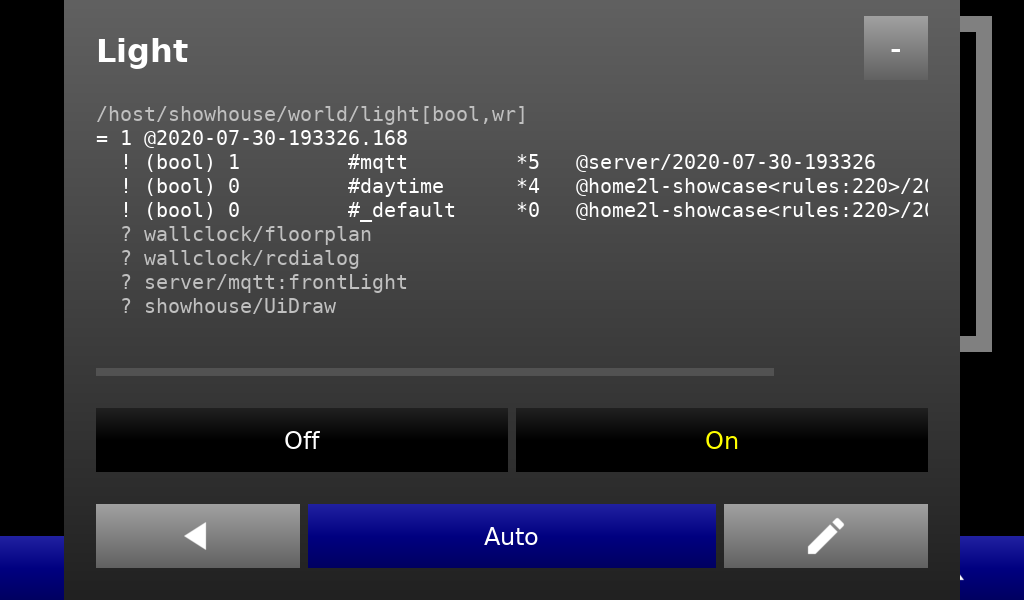
\includegraphics[width=0.7\linewidth]{figs/wallclock-floorplan-light-mqtt.png}
  \caption[l]{Details of the front door light resource with an active MQTT request}
  \label{fig:tutorial-floorplan-light-mqtt}
\end{figure}



%%%%%%%%%%%%%%%%%%%%%%%%%%%%%%%%%%%%%%%%%%%%%%%%%%%%%%%%%%%%
\subsection{Importing a (Virtual) Mailbox Sensor}
\label{sec:tutorial-mqtt-imports}
%%%%%%%%%%%%%%%%%%%%%%%%%%%%%%%%%%%%%%%%%%%%%%%%%%%%%%%%%%%%

This section demonstrates how MQTT-enabled devices are integrated into the \textit{Home2L} set of resources.

The MQTT gateway is configured to import a resource (\lst{/host/server/mqtt/mailbox} or \lst{/alias/mailbox}),
a sensor device that indicates whether there is mail in the mailbox.

The device publishes the state via the MQTT topic \lst{mailbox/state}. Also, the device publishes its aliveness via the MQTT topic \lst{mailbox/online} and sets a last-will-and-testament (LWT) message accordingly.

Since a real sensor device may not be available to you at the time you run this tutorial, we will simulate
the device by publishing its messages manually. To get started, the \lst{home2l demo} script has already
published \lst{mailbox/online=1} and \lst{mailbox/state=0} before, which corresponds to a working device
indicating that the mailbox is empty.

\begin{itemize}[$\blacktriangleright$]

\item
  Open a new terminal window and run the following command to observe the mailbox resource:
  \begin{lstlisting}[language=bash]
    $ DOCKER home2l follow mailbox
    Subscriber 'home2l-showcase<shell:428>/shell'
      /host/server/mqtt/mailbox ?
    : /host/server/mqtt/mailbox = 0 @2021-11-21-174036.585
    : /host/server/mqtt/mailbox connected
  \end{lstlisting}

\item
  In the \textit{MQTT command} window, enter
  \begin{lstlisting}[language=bash]
    $ mosquitto_pub -r -t mailbox/state -m 1
  \end{lstlisting}
  and see that the mail icon appears in the \textit{WallClock} floor plan to indicate that new mail arrived.
  Enter
  \begin{lstlisting}[language=bash]
    $ mosquitto_pub -r -t mailbox/state -m 0
  \end{lstlisting}
  and see that the mailbox icon disappears again.

\item
  Enter
  \begin{lstlisting}[language=bash]
    $ mosquitto_pub -r -t mailbox/online -m 0
  \end{lstlisting}
  to simulate that the sensor device has a failure and gets disconnected. The mail icon with a red frame
  appears in the floor plan to indicate that the device is not working properly.
  Finally enter
  \begin{lstlisting}[language=bash]
    $ mosquitto_pub -r -t mailbox/online -m 1
  \end{lstlisting}
  to simulate that the device is alive again. The icon disappears.

\end{itemize}



%%%%%%%%%%%%%%%%%%%%%%%%%%%%%%%%%%%%%%%%%%%%%%%%%%%%%%%%%%%%
\subsection{Import Your Own Real Hardware!}
\label{sec:tutorial-mqtt-real}
%%%%%%%%%%%%%%%%%%%%%%%%%%%%%%%%%%%%%%%%%%%%%%%%%%%%%%%%%%%%

This section describes how to replace the outdoor light of the \textit{ShowHouse} with a real MQTT-enabled power switch. It has been tested with a \textit{Delock 11826} device running \href{https://tasmota.github.io/docs}{Sonoff-Tasmota 6.7.1} firmware. For other devices, the file \reftool{home2l.conf} contains commented \refenv{mqtt.import.<ID>} examples that may be used and adapted to match your own actual device. In general, any type of on/off switch that is able to report its state can be used here.

At your choice, it possible to use either your own MQTT broker or the MQTT broker of the demo system.

\warnbox{
  This tutorial step involves restarting the Docker container in ''host networking'' mode. This means that
  all listening network ports of the container bind to your host machine’s network, with no network isolation.
  To avoid conflicts, no process on your host should use the \textit{Home2L} ports 4700 .. 4709 (see
  \lst{resources.conf}). Also, no MQTT broker should be running on your host machine if you use the container's
  broker and vice versa.
}

\begin{itemize}[$\blacktriangleright$]

\item
  Stop the running Docker container by pressing \textit{Q} and then \textit{Ctrl-D} in the
  \textit{ShowHouse} window.

\item
  Start the Docker image again as described Section~\ref{sec:tutorial-start}, but with the additional option
  \begin{lstlisting}
    ... --network host ...
  \end{lstlisting}
  inserted \textit{before the last argument}.

\item
  Open the file \lst{resources.conf} in a text editor:
  \begin{lstlisting}[language=bash]
    $ DOCKER_ROOT nano home2l.conf
  \end{lstlisting}

\item
  Search \textit{(F6)} for the line starting with \lst{mqtt.import.switchTasmota}, read the comments before
  this line and check that the topic matches the one configured in your device.

\item
  \textbf{To use your own MQTT broker:}
  \begin{enumerate}
    \item Edit the following line and replace \lst{localhost:1883} with the IP address and port of your broker.
      \begin{lstlisting}
      mqtt.broker = localhost:1883
      \end{lstlisting}
    \item Disable the internal broker by commenting out the following line in section ''Daemon'':
      \begin{lstlisting}
      daemon.run.mqtt   = /usr/sbin/mosquitto
      \end{lstlisting}
  \end{enumerate}

\item
  \textbf{To use the broker of the demo container:}
  \begin{enumerate}
    \item Make sure that no other MQTT broker is running on your host machine.
    \item Configure your device to use \lst{<IP>:1883} as the broker, where \lst{<IP>} is the IP address
      of your machine.
  \end{enumerate}

\item
  Save \textit{(Ctrl-S)} and exit \textit{(Ctrl-X)} the editor.

\item
  Edit the file \lst{resources.conf} in a text editor:
  \begin{lstlisting}[language=bash]
    $ DOCKER_ROOT nano resources.conf
  \end{lstlisting}
  For the front light, an alias is used. It presently points to a resource provided by the \textit{ShowHouse}
  and will now be changed to point to your MQTT device.

  Change the line defining the alias \lst{frontLight} as follows:
  \begin{lstlisting}
    A frontLight      server/mqtt/switchTasmota
  \end{lstlisting}

  Save \textit{(Ctrl-S)} and exit \textit{(Ctrl-X)} the editor.

\item
  To make these changes effective, all tools must be restarted. Quit the \textit{WallClock} and
  the \textit{ShowHouse} (press ''Q''). Then run the following commands in the \textit{ShowHouse} window:
  \begin{lstlisting}[language=bash]
    $ home2l demo stop   # stop background services
    $ home2l demo run
  \end{lstlisting}

  \textbf{Your done!}

\item
  Interact with the \textit{ShowHouse} or \textit{WallClock} and see how the front door light
  is operated by your device!

\end{itemize}






%%%%%%%%%%%%%%%%%%%%%%%%%%%%%%%%%%%%%%%%%%%%%%%%%%%%%%%%%%%%%%%%%%%%%%%%%%
\clearpage
\section{Writing Automation Rules}
\label{sec:tutorial-rules}
%%%%%%%%%%%%%%%%%%%%%%%%%%%%%%%%%%%%%%%%%%%%%%%%%%%%%%%%%%%%%%%%%%%%%%%%%%


\textit{Home2L} automation rules are normal Python scripts.
They can be tested separately from already existing rules files and later be merged into them.
Section~\ref{sec:tutorial-rules-example} describes this process for an example.
Section~\ref{sec:tutorial-rules-python} gives an in-depth introduction to the
\theapipython{} by means of an interactive Python session.
Finally, the supplied \reftool{rules-showhouse} file will be inspected and extended in Section~\ref{sec:tutorial-rules-showhouse}.





%%%%%%%%%%%%%%%%%%%%%%%%%%%%%%%%%%%%%%%%%%%%%%%%%%%%%%%%%%%%
\subsection{Your Own Front Light Automation}
\label{sec:tutorial-rules-example}
%%%%%%%%%%%%%%%%%%%%%%%%%%%%%%%%%%%%%%%%%%%%%%%%%%%%%%%%%%%%


In this section, we will deactivate the provided \reftool{rules-showhouse} script and write
an own rules file to control the front light of the show house.
The \textit{Home2L} Python package offers a number of different techniques to implement automation rules (see Section~\ref{sec:rules-events}). In this section, some of them are demonstrated and sometimes compared to alternative solutions for the same problem.


\begin{itemize}[$\blacktriangleright$]

\item
  In the \textit{ShowHouse} window, quit (''Q'') the \textit{ShowHouse} tool.
  Then stop the \textit{Home2L} daemon together with \reftool{rules-showhouse} script and start
  \reftool{home2l-showhouse} again:
  \begin{lstlisting}[language=bash]
    $ home2l demo stop
    $ home2l showhouse
  \end{lstlisting}

  This will stop the server instance, too. In consequence, the weather displays disappear and the mailbox
  icon shows an error due to the missing MQTT driver. This is no problem.

  Then push ''M'' and ''D'' and verify that the front light no longer switches automatically on
  motion at night.

\item
  Start a command shell in the Docker container (or switch to the one still open) and set
  the \textit{Home2L} environment variables:
  \begin{lstlisting}[language=bash]
    $ DOCKER bash
    $ . /opt/home2l/env.sh   # to set the Python search path
  \end{lstlisting}

\end{itemize}


\subsubsection*{A First Rules Script}

\begin{itemize}[$\blacktriangleright$]

\item
  Open a text editor to create a new file \lst{myrules}:
  \begin{lstlisting}[language=bash]
    $ cd
    $ nano myrules
  \end{lstlisting}
  with the following contents:
  \begin{lstlisting}
    #!/usr/bin/python3

    from home2l import *

    # Init the Home2L package ...
    Home2lInit ()

    # Get some resource handles ...
    rcDaylight = RcGet ("daylight")
    rcRain = RcGet ("weatherWarning")
    rcMotion = RcGet ("motion")
    rcLight = RcGet ("frontLight")

    # Set default request ...
    rcLight.SetDefault (0)

    # Rule to acrivate the light on motion ...
    @onUpdate (rcMotion)
    def LightOnMotion (motion):
      if motion == True: rcLight.SetRequest (1, attrs = '#motion *3')
      else: rcLight.DelRequest ('#motion', '5s')
      print ("Hi there - motion = " + str (motion))

    # Go ahead ...
    Home2lRun ()
  \end{lstlisting}

  The lines following \lstf{\# Get some resource handles...} lookup some resource
  objects and place them in Python variables. This is good practice, but not strictly
  necessary. The rules later would also accept strings containing the resource identifiers (URI).

  The next lines are the actual rules area. There are two rules controlling the front light (\lst{rcLight}):
  The first one (\lst{rcLight.SetDefault (0)}) sets a default request to let the light turn off (0)
  if no other request is active.

  The second rule consists of the funtion \lstf{LightOnMotion()}. The decorator \lstf{@onUpdate (rcMotion)}
  lets the function be called whenever the value or state of \lst{rcMotion} changes
  (see Section~\ref{sec:rules-actions-onupdate}).
  The new resource value is passed as the function argument (\lst{motion}). Whenever called with
  \lstf{motion == True}, a request is set to activate the light. The attributes \lstf{attrs = '\#motion *3'}
  specify a request ID of \textit{''motion''} and a priority of 3. If called with \lstf{motion == False}
  (or \lstf{motion == None}), the request is deleted with a delay of 5 seconds (\lstf{'5s'}).

  The \lstf{print()} statement just prints some status information on the console to indicate when the
  triggered function is called.

\item
  Save the file and exit the editor. Then make it executable and run it:
  \begin{lstlisting}[language=bash]
    $ chmod a+x myrules
    $ ./myrules
  \end{lstlisting}
  In the \textit{ShowHouse} windows, push ''M'' and see that the front light switches on on
  motion and stays on for 5 seconds.

\end{itemize}

\infobox{
  To watch the requests being added and deleted, you may use the \textit{WallClock} and open the resource
  dialog for the front light in detail view (see Figure~\ref{fig:tutorial-floorplan-light-mqtt}).
}


\subsubsection*{Using Connectors}

\begin{itemize}[$\blacktriangleright$]

\item
  The automation rule for activating the light on motion and switching it off 5 seconds later can
  be formulated shorter by means of a \textit{connector} (see Section~\ref{sec:rules-actions-connectors}).

  Replace the decorated funtion (stating with \lstf{@onUpdate(rcMotion) ...}) with the following code:
  \begin{lstlisting}
    Connect (rcLight, rcMotion,
             lambda x: 1 if x == True else None,
             attrs = '#motion *3', delDelay = '5s')
  \end{lstlisting}

  The arguments in the first line define the destination and the source resource (\lstf{rcLight} and
  \lstf{rcMotion}, respectively).
  The \lstf{lambda x: ...} expression is the so-called \textit{transfer function} and defines
  how an \lst{rcMotion} value is translated into a request value for \lstf{rcLight}. In this
  example, the light is requested to be on (\lst{1}) if the motion sensor is active
  (\lstf{x = True}), whereas the request \lstf{\#motion} is deleted (\lstf{None}) in all
  other cases.
  The argument \lstf{attrs = '\#motion *3'} sets the request attributes (request ID of ''motion'' and
  a priority of 3, as before). The argument \lstf{delDelay = '5s'} sets the delay for request deletion to
  5~seconds.

\item
  Connectors may also have multiple sources.
  The following connector lets the light stay off at day time, but not during rainy weather:
  \begin{lstlisting}
    Connect (rcLight, (rcDaylight, rcRain),
             lambda day, rain: 0 if day == True and rain == False else None,
             attrs = '#daylight *4')
  \end{lstlisting}
  The request attributes define a priority of 4, so that \lstf{\#daylight} requests generated by this
  connector have a higher priority that \lstf{\#motion} requests set by the other rules.

  Add these lines to the script and run it! Manipulate the daylight and weather status in the
  \textit{ShowHouse} window to see how it works.

\end{itemize}


\subsubsection*{Going Further: Connectors with Explicit Functions}

\begin{itemize}[$\blacktriangleright$]

\item
  For complex connectors, putting the logic into a single lambda expression may be difficult or lead
  to incomprehensible code. The following code is equivalent to the previous example, but uses
  a Python decorator to build a connector around a named function:
  \begin{lstlisting}
    @connect (rcLight, (rcDaylight, rcRain), attrs = '#daylight *4')
    def LightOffDuringDay (daylight, rain):
      print ("LightOffDuringDay ({}, {}) called.".format (str(daylight), str(rain)))
      if daylight == True and rain == False: return 0
      return None
  \end{lstlisting}
  Similar to the \lst{@onUpdate} decorator, the function may contain arbitrary other Python
  code, and it is called whenever a value or state of any of the resources \lst{rcDaylight}
  or \lst{rcRain} changes.

  Replace the \lst{Connect (rcLight, (rcDaylight, rcRain), ...} statement with this alternative and
  run the script!
  Manipulate the daylight and weather status in the \textit{ShowHouse} window and verify the
  console output!

\item
  Stop the \textit{ShowHouse} script (press ''Q'') and start it again. Watch the console output
  of your \lst{myrules} script and see how it behaves if its resources get lost and reappear
  again.

\item
  Finally, stop your \lst{myrules} script (\textit{Ctrl-C}) and start the \textit{Home2L}
  daemon again:
  \begin{lstlisting}[language=bash]
    $ DOCKER demo start
  \end{lstlisting}

\end{itemize}





%%%%%%%%%%%%%%%%%%%%%%%%%%%%%%%%%%%%%%%%%%%%%%%%%%%%%%%%%%%%
\subsection{Digging Deeper into the Python API}
\label{sec:tutorial-rules-python}
%%%%%%%%%%%%%%%%%%%%%%%%%%%%%%%%%%%%%%%%%%%%%%%%%%%%%%%%%%%%


This section describes an interactive Python session to explore some technical aspects of the \theapipython.

\begin{itemize}[$\blacktriangleright$]

\item
  Switch to the command shell of the previous section or start a new one with:
  \begin{lstlisting}[language=bash]
    $ DOCKER bash
    $ . /opt/home2l/env.sh   # to set the Python search path
  \end{lstlisting}

\item
  Start a Python session:
  \begin{lstlisting}[language=bash]
    $ python3
    ...
    >>>
  \end{lstlisting}

\item
  Import the \textit{Home2L} package and initialize it:
  \begin{lstlisting}[language=python]
    >>> from home2l import *
    >>> Home2lInit ("interactive")
  \end{lstlisting}

\item
  Of course, online help and tab-completion is available for all commands. For example, try:
  \begin{lstlisting}[language=python]
    >>> help (RcGet)
    Help on function RcGet in module home2l:

    RcGet(uri, allowWait=False)
        RcGet(char const * uri, bool allowWait=False) -> CResource
        Lookup a resource by its URI and return a reference to it (shortcut for 'RcGetResource()').
  \end{lstlisting}

\item
  For the next steps it is necessary to start the \textit{Home2L} background tasks:
  \begin{lstlisting}[language=python]
    >>> Home2lStart ()
  \end{lstlisting}
  This ends the \textit{elaboration} phase and puts the \textit{Resources} library into a ready-to-use state.
  Optionally, the network server would be started if configured so (it is not enabled here).

\item
  To inspect the network environment and list the resources provided by, for example,
  \reftool{home2l-showhouse}, enter:
  \begin{lstlisting}[language=python]
    >>> RcHosts()
    ['home2l-showcase<interactive:1454>', 'server', 'showhouse', 'wallclock']
    >>> RcHostResources("showhouse")
    ['/host/showhouse/resource/bath-shades', '/host/showhouse/resource/bath-window',
    ...
    '/host/showhouse/timer/twilight/sunrise', '/host/showhouse/timer/twilight/sunset']
  \end{lstlisting}
  (Output is abbreviated for readability.)
\end{itemize}



\subsubsection*{Inspecting Resources and Reading Their Values}

\begin{itemize}[$\blacktriangleright$]

\item
  Now let us inspect some resources. The following sequence shows some commonly used commands to inspect
  resources and to obtain their values and states:
  \begin{lstlisting}[language=python]
    >>> rcNow = RcGet ("/local/timer/now")
    >>> rcNow
    (CResource) /host/home2l-showcase<interactive:567>/timer/now time ro
    >>> rcNow.PrintInfo()
    /host/home2l-showcase<interactive:567>/timer/now[time,ro] = 2020-01-11-150350 @2020-01-11-150350.000
      (no requests)
      (no subscriptions)
    >>> rcNow.ValueState()
    (CRcValueState) (time) 2020-01-11-144234
    >>> rcNow.Value()
    1578753761000
    >>> RcGet ("/local/timer/twilight/day").ValueState ()
    (CRcValueState) (bool) 1
    >>> RcGet ("/local/timer/twilight/day").Value ()
    True
  \end{lstlisting}

\item
  Let us try to do the same with a remote resource (say, the timer of the \textit{WallClock} instance):
  \begin{lstlisting}[language=python]
    >>> rcNow = RcGet ("/host/wallclock/timer/now")
    >>> rcNow
    (CResource) /host/wallclock/timer/now time ro
    >>> rcNow.ValueState ()
    (CRcValueState) (time) ?
    >>> rcNow.Value ()
    >>> str (rcNow.Value ())
    'None'
  \end{lstlisting}
  \textbf{Oh!} Why is the time unknown? Well, this and the previous sequence is lacking
  one important thing: To get values of resources, they must be subscribed to.
  The previous example only happened to work because we used local resources.

  To subscribe to the resource \textit{rcNow} enter:
  \begin{lstlisting}[language=python]
    >>> s = RcNewSubscriber ("mysub", rcNow)
    >>> s
    (CRcSubscriber) home2l-showcase<interactive:567>/mysub: /host/wallclock/timer/now
    >>> rcNow.PrintInfo()
    /host/wallclock/timer/now[time,ro] = 2020-01-11-145439 @2020-01-11-145439.007
      (no requests)
      ? home2l-showcase<interactive:567>/mysub
      ? wallclock/floorplan
    >>> rcNow.ValueState()
    (CRcValueState) (time) 2020-01-11-144911
  \end{lstlisting}
  Repeat the last command a couple of times to see that the value is now updated regularly.

\end{itemize}



\subsubsection*{Manipulating Resources}

\begin{itemize}[$\blacktriangleright$]

\item
  Resources can be manipulated by setting requests, for example, as follows:
  \begin{lstlisting}[language=python]
    >>> rcLight = RcGet ("frontLight")
    >>> rcLight.SetRequest (True, "*5 -5s")
  \end{lstlisting}
  The last command could also be written as:
  \begin{lstlisting}[language=python]
    >>> rcLight.SetRequest (True, priority = 5, t1 = "5s")
  \end{lstlisting}
  ... or both together like:
  \begin{lstlisting}[language=python]
  >>> RcSetRequest ("frontLight", "1 *5 -5s")
  \end{lstlisting}
  Actually, the methods \refapipython{CResource.SetRequest()} and \refapipython{RcSetRequest()}
  offer a wide range of possibilities to pass arguments. Values and attributes can be passed as strings
  or as values by named arguments or as a mixture thereof.

  Details can be found in the online documentation of these methods. To see details on passing
  request attributes, enter \lstf{help (RcSetRequest)} .

\end{itemize}



\subsubsection*{A Small Example Rule}

We will now define a simple rule on the command line and run it.
The rule monitors the current time and whenever the time changes, the value is printed out.

\begin{itemize}[$\blacktriangleright$]

\item
  Defining own drivers is only allowed before the \refapipython{Home2lStart()} call.
  Therefore, we restart the \textit{Home2L} package first:
  \begin{lstlisting}[language=python]
  >>> Home2lDone ()
  >>> Home2lInit ("interactive")
  \end{lstlisting}

\item
  Define the rule function as follows:
  \begin{lstlisting}[language=python]
  >>> rcNow = RcGet ("/host/showhouse/timer/now")
  >>>
  >>> @onUpdate (rcNow)
  §... def OnTimerUpdate ():
  §...   print (str (rcNow.ValueState ()))
  §...
  >>>
  \end{lstlisting}

  (Mind the indentation!)

  The function \textit{OnTime()} is prefixed with the decorator \refapipython{@onUpdate}, which makes it
  to be executed automatically whenever the passed resource \textit{rcNow} changes its value or state.

\item
  Start the \textit{Home2L} main loop:
  \begin{lstlisting}[language=python]
  >>> Home2lRun ()
  \end{lstlisting}
  Now, all rules (just one here) are active and executed.
  Interaction in the Python shell is no longer possible.

\item
  In the \textit{ShowHouse} window, stop the showhouse by pressing ''Q''.
  After a some time, start it again and watch the output in the \textit{Shell} window.
  \begin{lstlisting}[language=bash]
  $ home2l showhouse
  \end{lstlisting}
   In the output of your rule, you can see that the resource becomes unavailable and then available again.

\item
  In the \textit{Shell} window, press \textit{Ctrl-C} to stop the rules process and exit Python.

\end{itemize}



%%%%%%%%%%%%%%%%%%%%%%%%%%%%%%%%%%%%%%%%%%%%%%%%%%%%%%%%%%%%
\subsection{The \texttt{rules-showhouse} Automation Script}
\label{sec:tutorial-rules-showhouse}
\labeltool{rules-showhouse}
%%%%%%%%%%%%%%%%%%%%%%%%%%%%%%%%%%%%%%%%%%%%%%%%%%%%%%%%%%%%


The supplied automation script \reftool{rules-showhouse} (source tree: \refsrc{tools/etc/rules-showhouse}) contains a couple of example rules, the effects of which you may have already observed in previous tutorial steps. These are rules for
\begin{itemize}
  \item turning on the front light on motion at day time,
  \item closing the shades at night,
  \item controlling / dimming the the \textit{WallClock} display,
  \item opening the roof window at night on hot days for cooling,
  \item determining the \textit{presence} (use) state if the user selects the ''Auto'' mode.
\end{itemize}


\begin{itemize}[$\blacktriangleright$]

\item
  Changing the rules file requires root permissions. Define a macro for running commands as
  \textit{root} in the Docker container:
  \begin{lstlisting}[language=bash]
    $ alias DOCKER_ROOT="docker exec -ti --user=root home2l-showcase"
  \end{lstlisting}

\item
  Inspect and read the rules file:
  \begin{lstlisting}[language=bash]
    $ DOCKER_ROOT nano /opt/home2l/etc/rules-showhouse
  \end{lstlisting}

  (Color syntax highlighting can be switched off/on by pressing \textit{Alt-Y} in \textit{nano}.)

  Can you identify the rules mentioned above?

\item
  In the next steps, we will modify the rules script. To facilitate editing and debugging,
  we will run it in the foreground as long as we work on it.

  Stop the \textit{Home2L} daemon:
  \begin{lstlisting}[language=bash]
    $ DOCKER home2l demo stop
  \end{lstlisting}

  (The server instance will stop, too, and the weather displays disappear. This is no problem.)

  \infobox{
    Alternatively, if you only make little changes and do not want to stop the daemon,
    you may also just restart the rules script by killing it:
    \lstbox{\$ DOCKER\_ROOT pkill rules-showhouse}
    It will automatically be restarted by the \reftool{home2l-daemon}.
  }

\item
  Go to the code section controlling the front light.
  How is the light kept off at day time?
  What would you need to change to increase the light-on duration after a motion event?

  Change the rule so that after a motion event the light is switched on for 3 seconds instead of
  the original setting.

  After saving the file (\textit{Ctrl-S} in \textit{nano}), run the script in a new terminal window:
  \begin{lstlisting}
    $ DOCKER bash
    home2l@home2l-showcase:/opt/home2l/etc$ . /opt/home2l/env.sh
    home2l@home2l-showcase:/opt/home2l/etc$ ./rules-showhouse
  \end{lstlisting}

  Leave this terminal open for running the script in the following steps.

\item
  Assume you do not want to have all shades closed at night. Only those of the living room
  and the bedroom shall be closed, and those of the kitchen and bathroom left open.

  What needs to be changed in the rule script? Try it!

\item
  The rules for roof window cooling depends on a resource named \lst{rcTempDayMaxOutside}
  which models the maximum outside temperature of the day and is used to determine whether
  it is a hot day or not. Since it is not guaranteed that it is a hot day when you are reading
  this, this resource is mapped to a local signal in this demo.

  Identify the place where this internal signal resource is defined and change its value from
  20.0 (not hot) to 30.0 (hot day).

  Restart the rules script and try the roof window cooling functionality!
  See that the window opens during the night and the shades close during the day
  (press ''D'' in the \textit{ShowHouse} window to switch between day and night time).

  At night time, press ''R'' to simulate rain. See how the window closes to avoid damage!

\item
  The \textit{WallClock} can switch on and off the display or dim it, depending on its use. The display state
  is exposed by two boolean resources \refrc{ui/standby} and \refrc{ui/active}, which allow the display state to
  be controlled externally by rules. So far, a rule has been active which has simply kept the display active all the
  time. We now replace this with a more sophisticated rule that dims the display at night and if not used.

  \infobox{
    Like potentially any \textit{Home2L} application, the \textit{WallClock}
    exports a number of resources. For example, on \textit{Android} it can export
    the device's brightness sensor value or Bluetooth status. In this tutorial, we will use
    \refrc{ui/active}, \refrc{ui/standby} for controlling the UI state and optionally
    \refrc{ui/mute} to mute the audio player.
  }

  Identify the rule for keeping the \textit{WallClock} display permanently active
  \begin{lstlisting}
    @daily("wallclock")
    def WallClockDisplay (host):
      ...
  \end{lstlisting}
  and deactivated it by commenting out its \refapipython{@daily} decorator:
  \begin{lstlisting}
    # @daily("wallclock")
    def WallClockDisplay (host):
      ...
  \end{lstlisting}

  To make this change effective, it necessary to remove its already existing permanent requests:
  \begin{lstlisting}[language=bash]
    $ DOCKER home2l shell -e "c /host/wallclock/ui; r- active rules; r- standby rules"
  \end{lstlisting}

  After some time (at most 10 seconds, see the \refenv{ui.standbyDelay} setting in
  \reftool{home2l.conf}), the \textit{WallClock} UI should dim or turn off
  completely. Clicking on it re-activates it for some time. You may test
  this now, but should then wait again until the screen dims. After that,
  you should not click into the \textit{WallClock} window anymore.

\item
  Replace the \lst{WallClockDisplay} rule with a new one, which switches the display on
  at day time or whenever the door is unlocked in order to remind the user to
  lock it over night:
  \begin{lstlisting}
    @onUpdate (rcDaylight, "doorLock")
    def WallClockDisplayNew (daylight, lock):
      print ("### daylight = {}, lock = {}".format (str (daylight), str (lock)))
      if daylight == False and lock != True:
        rcWallClockActive.SetRequest (1)
      else:
        rcWallClockActive.DelRequest ()
  \end{lstlisting}

  (Mind the indentation!)

  The first line (\refapipython{@onUpdate()}), a Python \textit{decorator},
  causes the function \textit{WallClockDisplayNew()} to be called whenever
  the value of any of the supplied resources changes. Depending on these values, a
  request is set or deleted to switch the display active or not.

  The line \lstf{print (...)} just serves debugging purposes and is not strictly necessary.

\item
  Add a new rule to mute the music player for 5 seconds if motion is detected in
  front of the house:
  \begin{lstlisting}
    @onEvent ("motion")
    def MuteOnMotion (ev, rc, vs):
      if ev == rceValueStateChanged and vs.Value () == True:
        RcSetRequest ("/host/wallclock/ui/mute", "1 -5s")
  \end{lstlisting}
  For demonstration purposes, this example uses the \refapipython{@onEvent()} decorator,
  which allows to track all events precisely.

%  An alternative to this rule with similar semantics is:
%  \begin{lstlisting}
%    Connect ("/host/wallclock/ui/mute", "motion", lambda x: 1 if x == True else None, value = 1, delDelay = "5s")
%  \end{lstlisting}

\item
  Finally, start the \textit{Home2L} daemon again, which also starts your modified rules script
  in the background:
  \begin{lstlisting}[language=bash]
    $ DOCKER home2l demo start
  \end{lstlisting}

\end{itemize}





%%%%%%%%%%%%%%%%%%%%%%%%%%%%%%%%%%%%%%%%%%%%%%%%%%%%%%%%%%%%%%%%%%%%%%%%%%
\clearpage
\section{\textit{Brownies}: Integrating Do-It-Yourself Hardware}
\label{sec:tutorial-brownies}
%%%%%%%%%%%%%%%%%%%%%%%%%%%%%%%%%%%%%%%%%%%%%%%%%%%%%%%%%%%%%%%%%%%%%%%%%%


This section will introduce the \textit{Brownies} framework and guide you to integrate an \textit{ATtiny} microcontroller with an LED into the \textit{ShowHouse}. Up to now, the \textit{ShowHouse} only contained virtual hardware. We will change this and replace the outdoor previously simulated by the \reftool{home2l-showhouse} with a real light!

This section expects basic knowledge in electronics and microcontroller programming, the target audience are people planning  to build their own hardware. It is recommended to read the overview section of Chapter~\ref{ch:brownies} before proceeding.

\eshockdisclaimer



\subsection{Prerequisites}
\label{sec:tutorial-brownies-prerequisites}

The following additional hardware is required for this part of the tutorial:
\begin{itemize}
  \item an \textit{ATtiny85} microcontroller,
  \item basic equipment for programming the \textit{ATtiny85}
        (for example, an \textit{AVRISP mkII} programmer and \textit{avrdude(1)} ),
  \item an \textit{ELV USB-i2c} interface
        \textit{(or some other \textit{i2c} host interfaces -- see info box below)},
  \item a breadboard,
  \item an LED,
  \item a $220\Omega$ resistor.
\end{itemize}

\infobox{
  \textbf{Using a Different \textit{i2c} Adapter}

  In general, this tutorial can be run with any \textit{i2c} host adapter supported as a Linux
  \textit{i2c} device (kernel module \lstf{i2c\_dev}, typical device names are \lst{/dev/i2c-*}).
  Just note:
  \begin{enumerate}
    \item The adapter must support \textit{clock stretching}.
    \item The tutorial assumes a power supply of 5V coming from the adapter or host. Other supply voltages
          between 2V and 5V are possible, too. If a supply voltage other than 5V is used, the only
          required change in the circuit is LED pre-resistor, which should be adapted accordingly.
  \end{enumerate}
}



\subsection{Initializing the Microcontroller}
\label{sec:tutorial-brownies-init}

The first step is to prepare the microcontroller. This is done with your favorite programming tool and should be done before the device is built into the circuit. This step only needs to be done once. After that, the microcontroller can be installed, and the programmer is no longer needed.

\begin{itemize}[$\blacktriangleright$]
  \item
    Copy the initialization image from the Docker container to your host:
    \begin{lstlisting}[language=bash]
      $ docker cp home2l-showcase:/opt/home2l/share/brownies/init.t85.elf .
    \end{lstlisting}

  \item
    On your host PC, program the \textit{ATtiny} microcontroller using your programmer and software
    of your choice. The initialization image \lst{init.t85.elf} contains
    \begin{itemize}
      \item the \textit{maintenance} firmware,
      \item initial EEPROM contents,
      \item initial fuse bits (like factory defaults, but with self-programming enabled).
    \end{itemize}
    Make sure that you program all of them.

    For example, with \textit{avrdude} and an \textit{AVRISP mkII} programmer, the command is:
    \begin{lstlisting}[language=bash]
      $ avrdude -c avrisp2 -p t85 \
      §    -U  hfuse:w:init.t85.elf \
      §    -U  efuse:w:init.t85.elf \
      §    -U eeprom:w:init.t85.elf \
      §    -U  flash:w:init.t85.elf
    \end{lstlisting}

\end{itemize}


\infobox{
  This is usually the last time you need your programmer. All other programming --
  installing the operational firmware, configuring the device -- can be done with the
  \textit{Home2L Brownies} maintenance tool (\reftool{home2l-brownie2l}).
}



\subsection{Building the Circuitry}
\label{sec:tutorial-brownies-circuit}

The demo circuit is minimal \textit{bus tree} with a single device node (\textit{Brownie}). This device has an LED as an acting output.

\begin{itemize}[$\blacktriangleright$]
  \item
    Build your \textit{bus tree} circuitry on the breadboard as shown in
    Figure~\ref{fig:tutorial-circuit}.
    \begin{itemize}
      \item The TWI slave port signals \textit{twi\_sl\_scl} and \textit{twi\_sl\_sda} are connected
            to the \textit{USB-i2c} adapter.
      \item The LED is driven by signal \textit{gpio0} (pin 6 / PB1).
      \item Power supply is provided by the \textit{USB-i2c} adapter.
    \end{itemize}
\end{itemize}

\infobox{
  The complete signal-to-pin assignments for the \textit{ATtiny85} are shown in
  Figure~\ref{fig:brownies-pinout-t85}.
}

\begin{figure}[ht]
  \centering
  \figsvg[inkscapearea=page]{figs/tutorial-circuit.svg}
  \caption[l]{Tutorial circuitry for a minimal \textit{Brownie bus tree} with one \textit{ATtiny85} microcontroller}
  \label{fig:tutorial-circuit}
\end{figure}



\subsection{Testing and Configuring the Hardware Using \texttt{home2l-brownie2l}}
\label{sec:tutorial-brownies-brownie2l}

Now we will test the hardware step-by-step and then prepare the \textit{Brownie} for productive use.

\begin{itemize}[$\blacktriangleright$]
  \item
    Stop the running Docker container by pressing \textit{Q} and then \textit{Ctrl-D} in the \textit{ShowHouse} window.

  \item
    Connect the \textit{i2c} interface adapter to the PC.

  \item
    Start the Docker image again as described Section~\ref{sec:tutorial-start},
    but with the additional option
    \begin{lstlisting}
      ... --device /dev/ttyI2C ...
    \end{lstlisting}
    inserted \textit{before the last argument}. Replace \textit{''/dev/ttyI2c''} with the actual
    device name of your \textit{i2c} adapter (probably \textit{''/dev/ttyUSBx''} in case of the ELV
    adapter, else like \textit{''/dev/i2c-x''}).

  \item
    The demo system expects the \textit{i2c} device to be named \textit{''/dev/i2c''}.
    Set a symlink link accordingly:
    \begin{lstlisting}[language=bash]
      $ DOCKER_ROOT ln -s /dev/ttyI2C /dev/i2c
    \end{lstlisting}
    Again, replace \textit{''/dev/ttyI2c''} with the actual device name of your \textit{i2c} adapter.

  \item
    Start the \textit{Brownie maintenance tool}:
    \begin{lstlisting}[language=bash]
      $ DOCKER home2l brownie2l
      home2l-brownie2l v0.9-233 (2020-01-26) by Gundolf Kiefer

      Connected to '/dev/i2c' (ELV USB-i2c).
      Read database file '/opt/home2l/etc/brownies.conf'.

      brownie2l>
    \end{lstlisting}

    \textit{This is a check if your adapter is working from within your ShowCase environment.
    If it has not been detected, either your adapter is incompatible, or you have a software
    problem on your PC. If so: Fix it now. You may disconnect the adapter from the circuit for this.}

    \textit{Verify that your \textit{i2c} adapter has been detected successfully!}

  \item
    Run an \textit{i2c} bus scan:
    \begin{lstlisting}[language=brownie2l]
      brownie2l> scan
      007 new                      init.t85 v0.9.233*
    \end{lstlisting}

    \textit{This is a check if your ATtiny has been programmed and your circuitry been connected
    correctly. If the scan takes longer than a few seconds, there is a general problem with the bus
    (e.g. missing pull-ups, open wires, missing power supply).}

    \textit{Verify that your device has been detected as shown above! (The firmware version may differ.)}

  \item
    Open the device:
    \begin{lstlisting}[language=brownie2l]
      brownie2l> open 7
      007 new
              Device:   ATTiny85
              Firmware: init.t85 v0.9.233*
              Features: maintenance
              Config:
    \end{lstlisting}
    The output lists the features and indicates that the maintenance system is running.

  \item
    Download the operational firmware for the preconfigured \textit{Brownie} ''showgarden'':
    \begin{lstlisting}[language=brownie2l]
      brownie2l> program -d showgarden

      Segments in '/opt/home2l/share/brownies/ahub.t85.elf':
         FLASH  : 0a00 - 15cc (3020 bytes)
        (SRAM)  : 0060 - 00e2 (130 bytes)
        (EEPROM): 0000 - 0032 (50 bytes)

      (Re-)program FLASH of device 007 with this? (y/N) §y

      Flashing device 007 with '/opt/home2l/share/brownies/ahub.t85.elf' ...
        0a00 - 15cc (3020 bytes) ... verifying ... OK
    \end{lstlisting}

  \item
    Configure the device according to the preconfigured database (\reftool{brownies.conf}):
    \begin{lstlisting}[language=brownie2l]
      brownie2l> config -d showgarden

      007 showgarden
        adr=008 id=showgarden fw=ahub.t85

      Write back this configuration and reboot node 007? (y/N) y
      Writing ID and config ... verifying ID ... verifying config ... OK
      Rebooting ... OK
    \end{lstlisting}

  \item
    Activate and boot the operational system:
    \begin{lstlisting}[language=brownie2l]
      brownie2l> boot -o
      Switching device 008 to OPERATIONAL firmware (block 0x28, adr=0x0a00) ... Activating and rebooting ... OK
    \end{lstlisting}

  \item
    Perform another (verbose) bus scan to see the device with its new identity:
    \begin{lstlisting}[language=brownie2l]
      brownie2l> scan -v
      008 showgarden               ahub.t85 v0.9.233*
              Device:   ATTiny85
              Features: twihub
              GPIOs:    0
              Config:   hub_maxadr=000 hub_speed=0
    \end{lstlisting}

  \item
    We will now access the device directly to switch on and off the LED. The LED is connected to GPIO \#0.
    To switch on the LED, write a ''1'' into the first GPIO register:
    \begin{lstlisting}[language=brownie2l]
      brownie2l> write gpio-0 1
      reg(0x02) <- 0x01
    \end{lstlisting}
    To switch the LED off again, enter:
    \begin{lstlisting}[language=brownie2l]
      brownie2l> write gpio-0 0
      reg(0x02) <- 0x00
    \end{lstlisting}

    \infobox{
      Like the \textit{Home2L Shell}, \reftool{home2l-brownie2l} has an exhaustive online help.
      Entering
      \lstbox{brownie2l> help [<command>]}
      will display a list of all commands or help on a particular command.
      The complete register map including the exact name and address of the GPIO register used above
      is listed in the help of the \textit{''write''} (or \textit{''read''}) command:
      \lstbox{brownie2l> help write}
    }

  \item
    During the session, \reftool{home2l-brownie2l} continuously collects communication statistics.
    Display the statistics collected so far:
    \begin{lstlisting}[language=brownie2l]
      brownie2l> statistics

      TWI Communication Statistics
      ============================

      Sending                       | Fetching                     |
      Ops         Retries  Failures | Ops        Retries  Failures |
      ------------------------------------------------------------------------------
            706       508       254 |      452         0         0 | Reason
      ------------------------------------------------------------------------------
                      508       254 |                  0         0 |  8 No device at given address

      Statistics on 'brownie2l@home2l-showcase<303>' since 2020-01-26-195435.023.

    \end{lstlisting}
    The errors shown here were caused by the \textit{''scan''} commands as they tried to contact non-existing
    devices. The 452 (=706-254) successful operations are related to the remaining activities, mainly
    firmware programming and configuration.

    Reset the statistics:
    \begin{lstlisting}[language=brownie2l]
      brownie2l> statistics -r
    \end{lstlisting}
    Then turn the LED on and off again and print the statistics again:
    \begin{lstlisting}[language=brownie2l]
      brownie2l> w gpio-0 1
      reg(0x02) <- 0x01
      brownie2l> w gpio-0 0
      reg(0x02) <- 0x00
      brownie2l> statistics

      TWI Communication Statistics
      ============================

      Sending                       | Fetching                     |
      Ops         Retries  Failures | Ops        Retries  Failures |
      ------------------------------------------------------------------------------
              2         0         0 |        2         0         0 | Reason
      ------------------------------------------------------------------------------

      Statistics on 'brownie2l@home2l-showcase<303>' since 2020-01-26-195715.520.
    \end{lstlisting}
    Each of the \textit{''w''} commands caused one operation, which is visible in the output.
\end{itemize}



\subsection{Installing the \textit{Brownie} in the Show House}
\label{sec:tutorial-brownies-resources}

Now we will integrate the \textit{Brownie} into the \textit{Home2L} cluster of the demo system.
Let us replace the outdoor light of the \textit{ShowHouse} with a real light -- your LED!

\begin{itemize}[$\blacktriangleright$]
  \item
    Quit \reftool{home2l-brownie2l} (\textit{Ctrl-D}) and edit the file \lst{home2l.conf} in a text editor:
    \begin{lstlisting}[language=bash]
      $ DOCKER_ROOT nano home2l.conf
    \end{lstlisting}
    In section ''[server]'', add the following line to enable the ''brownies'' driver for the
    server instance:
    \begin{lstlisting}
      drv.brownies = 1
    \end{lstlisting}
    \textit{After} the lines following ''[brownie2l,server]'', add:
    \begin{lstlisting}
      [brownie2l]
      br.link = "="
    \end{lstlisting}
    This directs \reftool{home2l-brownie2l} for the future to attach to the running driver instead
    of accessing the \textit{i2c} device directly (otherwise, conflicts would occur if both try to
    access the same device).

  \item
    Edit the file \lst{resources.conf} in a text editor:
    \begin{lstlisting}[language=bash]
      $ DOCKER_ROOT nano resources.conf
    \end{lstlisting}
    For the front light, an alias is used. It presently points to a resource provided by the \textit{ShowHouse}
    and will now be changed to point to the \textit{Brownie's} GPIO resource connected to the LED.

    Change the line defining the alias \lst{frontLight} as follows:
    \begin{lstlisting}
      A frontLight      server/brownies/showgarden/gpio/00
    \end{lstlisting}

  \item
    To make these changes effective, all tools must be restarted. Quit the \textit{WallClock} and
    the \textit{ShowHouse} (press ''Q''). Then run the following commands in the \textit{ShowHouse}
    window:
    \begin{lstlisting}[language=bash]
      $ home2l demo stop   # stop background services
      $ home2l demo run
    \end{lstlisting}

    \textbf{Your done!}

  \item
    Interact with the \textit{ShowHouse} or \textit{WallClock} and see how the outdoor light
    is operated by your LED!

\end{itemize}





%%%%%%%%%%%%%%%%%%%%%%%%%%%%%%%%%%%%%%%%%%%%%%%%%%%%%%%%%%%%%%%%%%%%%%%%%%
\clearpage
\section{\textit{WallClock} Gadgets: The Music Player}
\label{sec:tutorial-wallclock}
%%%%%%%%%%%%%%%%%%%%%%%%%%%%%%%%%%%%%%%%%%%%%%%%%%%%%%%%%%%%%%%%%%%%%%%%%%


The \textit{WallClock}'s music player is a \href{https://www.musicpd.org/}{Music Player Daemon (MPD)} client, optimized for a home setup with multiple \textit{WallClocks} in different rooms and multiple music machines.

\begin{itemize}[$\blacktriangleright$]
\item
  Copy some of your favorite music files into the Docker container:
  \begin{lstlisting}[language=bash]
    $ docker cp /your/favorite/album/ home2l-showcase:/var/opt/home2l/mpd/music/
  \end{lstlisting}
  Replace ''/your/favorite/album/'' with a directory containing some music files on your computer.
  It should contain about $1 - 50$ \textit{mp3} or \textit{flac} files.
  % Alternatively, you can download some free music from \url{https://freemusicarchive.org}, for example.

\item
  Push the \textit{''Music''} button in the \textit{WallClock} window.

\item
  In the navigation pane (right half of the screen), navigate to your
  favorite song. Pushing the title bar of the navigation pane will
  navigate up or switch between the local database and playlists.

\item
  Select your favorite song, push the play button and enjoy!

\end{itemize}


\infobox{
  \textbf{Audio Output Troubleshooting}

  The integrated music player relies on a working MPD (should have been installed so far)
  and a working ALSA device (\code{/dev/snd}).

  The MPD configuration file is located in \lst{/opt/home2l/etc/mpd-showstage.conf}. It
  should work out-of-the-box, but may be further adapted to your preferences.
  By default, the audio output is directed to the default ALSA playback channel.

  To play audio from the Docker container, it is important that on your host system
  \textit{no other process} uses the sound card.

  Such processes can be identified by:
  \lstbox{
    \# lsof 2>/dev/null | grep /dev/snd | grep -v 5000
  }

  To test if audio playback is working inside your container / VM, run:
  \lstbox{
    \$ speaker-test -t sine
  }

  To adjust the volume or unmute the device, run:
  \lstbox{
    \$ alsamixer
  }

  To update the music database manually after you have copied files into the music directory:
  \lstbox{
    \$ mpc -h localhost update
  }

  Make sure that the \textit{MPD} instance with the \textit{Home2L} configuration has been started properly
  and that the default instance is off (does not apply to the Docker container):
  \lstbox{
    \$ sudo systemctl disable mpd \\
    \$ sudo systemctl stop mpd \\
    \$ sudo systemctl restart home2l
  }
}





%%%%%%%%%%%%%%%%%%%%%%%%%%%%%%%%%%%%%%%%%%%%%%%%%%%%%%%%%%%%%%%%%%%%%%%%%%
\section{\textit{WallClock} Gadgets: The Family Calendar}
\label{sec:tutorial-calendar}
%%%%%%%%%%%%%%%%%%%%%%%%%%%%%%%%%%%%%%%%%%%%%%%%%%%%%%%%%%%%%%%%%%%%%%%%%%


The calender applet uses \textit{remind(1)} as a backend and thus
supports its syntax for specifying events.

\begin{itemize}[$\blacktriangleright$]
\item
  Start the applet by pushing ''Calendar'' on the main screen.
\item
  Explore the calendar UI by navigating to different dates (e.g.~your wife's
  next birthday or your next anniversary).
\item
  Select an event in the right pane and modify it (e.g.~change its time
  or text).
\item
  Select a day in the left pane and add a new one-time appointment for
  Julian, for example (enter/keep your own date at the beginning):
  \begin{lstlisting}
    2020-12-23 at 19:00 dur 2:00 MSG Meet Henry; Murphy's Pub
  \end{lstlisting}
\end{itemize}





%%%%%%%%%%%%%%%%%%%%%%%%%%%%%%%%%%%%%%%%%%%%%%%%%%%%%%%%%%%%%%%%%%%%%%%%%%
\clearpage
\section{Going Further}
\label{sec:tutorial-goingfurther}
%%%%%%%%%%%%%%%%%%%%%%%%%%%%%%%%%%%%%%%%%%%%%%%%%%%%%%%%%%%%%%%%%%%%%%%%%%


To learn more about the capabilities of the \textit{Home2L} suite, we
suggest to look into the configuration files and source code of the
tutorial.

\begin{itemize}[$\blacktriangleright$]

\item
  The supplied rules file has already been inspected in Section~\ref{sec:tutorial-rules}
  (source tree: \refsrc{tools/etc/rules-showhouse}):
  \begin{lstlisting}[language=bash]
    $ DOCKER nano /opt/home2l/etc/rules-showhouse
  \end{lstlisting}

\item
  Inspect and read the \textit{ShowHouse} source file
  (source tree: \refsrc{resources/home2l-showhouse}):
  \begin{lstlisting}[language=bash]
    $ DOCKER nano /opt/home2l/bin/home2l-showhouse
  \end{lstlisting}

  It contains an example for a resource driver implemented in Python,
  namely for the \textit{ShowHouse} gadgets and the keyboard input. The
  latter is a bit more sophisticated and involves a background thread.

  The ASCII art visualization is refreshed whenever necessary, but not
  unnecessarily often. This is achieved by implementing the drawing function as a rule.

\item
  Inspect and read the main configuration file (source tree: \refsrc{tools/etc/home2l.conf}):
  \begin{lstlisting}[language=bash]
    $ DOCKER nano /opt/home2l/etc/home2l.conf
  \end{lstlisting}

\end{itemize}

\textbf{The following major components are not (yet) covered in the tutorial:}
\begin{enumerate}

  \item
    Setting up an intercom system with multiple room video phones and multiple
    doorphones using \href{https://www.asterisk.org/}{Asterisk}, \reftool{home2l-wallclock}
    and \reftool{home2l-doorman} instances. The author has such a system in productive use for
    a few years now, but it requires some technical expertise (and perhaps some patience) to set it up.

\end{enumerate}





%%%%%%%%%%%%%%%%%%%%%%%%%%%%%%%%%%%%%%%%%%%%%%%%%%%%%%%%%%%%%%%%%%%%%%%%%%
\clearpage
\section{Alternative Ways of Running the Tutorial}
\label{sec:tutorial-nodocker}
%%%%%%%%%%%%%%%%%%%%%%%%%%%%%%%%%%%%%%%%%%%%%%%%%%%%%%%%%%%%%%%%%%%%%%%%%%


\subsection{Native Installation}
\label{sec:tutorial-nodocker-native}

Of course, the \textit{ShowCase} demo system can be run natively on a Linux machine.

The official reference for building and installing the \textit{Home2Ls} is the \refsrc{Dockerfile}, which is both machine-readable and (at best effort) human-readable. It uses and is tested with the current stable release of \textit{Debian} as a base system. The \textit{Home2L} suite aims to minimize external dependencies, so that other distributions (Debian-based and others) should work with little problems.

In the \refsrc{Dockerfile}, the sections entitled ''Stage 1: Building'' and ''Stage 2: Runnable Demo Image'' contain all information required for building and installing the tools, respectively.

After installing the \textit{Home2L} suite, the demo environment as presented in Section~\ref{sec:tutorial-start} can be started with:
\begin{lstlisting}[language=bash]
  $ home2l demo run  # start all background services, the WallClock and home2l-showhouse
\end{lstlisting}


\subsection{Using a VirtualBox VM}
\label{sec:tutorial-nodocker-vbox}

It is also possible to run the demo in a VirtualBox VM. The project provides a
\refdoc{home2l-showcase-vbox.tar.gz}{preconfigured VM image} to facilitate this.

The following instructions have last been tested with \textit{VirtualBox 5.2.10} and \textit{Debian 9.6 (Stretch)}.

\begin{itemize}[$\blacktriangleright$]

\item
  Unpack the virtual machine into a new directory:
  \begin{lstlisting}[language=bash]
    $ mkdir home2l-tutorial
    $ cd home2l-tutorial
    $ tar xzf path/to/home2l-showcase-vbox.tar.gz
  \end{lstlisting}

\item
  Download and provide a Debian installation image as 'install.iso' in the same directory:
  \begin{lstlisting}[language=bash]
    $ wget https://cdimage.debian.org/debian-cd/current/i386/iso-cd/debian-9.6.0-i386-netinst.iso
        # Adapt the path as necessary. We need an i386 "netinst" image.
        # More information can be found on the Debian download page at
        # https://cdimage.debian.org.
    $ ln -s debian-*.iso install.iso
        # or rename the file (if your OS does not support symbolic links)
  \end{lstlisting}

  The virtual machine comes with an empty harddisk image and is configured
  to have the CD/DVD image \textit{'install.iso'} inserted in its optical drive.

\item
  Start \textit{VirtualBox}, select ''Machine $\rightarrow$ Add...'' and navigate to
  \begin{lstlisting}
    home2l-tutorial/home2l-showcase-vbox/home2l-showcase.vbox
  \end{lstlisting}
  to add the \textit{Home2L ShowCase VM} as new virtual machine.

\item
  Start the virtual machine:
  \begin{lstlisting}
  $ virtualbox --startvm home2l-showcase
  \end{lstlisting}
  The VM automatically boots from the Debian installation medium and runs the installer.

\item
  During the installation, accept all default settings or leave fields empty,
  except for the following options:
  \begin{enumerate}
    \item Select your country, language and keyboard layout as convenient for you.
    \item As a computer name, enter: \lstf{home2l-showcase}.
    \item Leave the root password empty (will allow \textit{home2l} to use \textit{sudo} for root access).
    \item As the name for the first normal user enter: \lstf{home2l}
    \item For user '\textit{home2l}' enter a password at your choice (and do not forget it!).
  \end{enumerate}

\item
  It is recommended to open this book inside the virtual machine.
  This will allow you to copy and paste terminal commands from this document into a terminal.

\item
  Optional: Install the \textit{VirtualBox Guest Additions}.

\item
  Install and run the \textit{Home2L} demo environment as sketched in
  Section~\ref{sec:tutorial-nodocker-native}.

\end{itemize}

\infobox{
  \begin{enumerate}
    \item
      The \textit{VirtualBox Guest Additions} are helpful for optimizing the screen resolution of the
      VM, but they are not required otherwise.
      If their installation fails, you can continue without them.
      In this case, you should move the PDF viewer to a second virtual desktop in the VM.
      Without it on the main desktop, a resolution of 1024x768 pixels is sufficient to run the
      tutorial.
    \item
      The VM has been pre-configured to use ''NAT'' networking. This is the most fail-safe setting and
      allows the VM to share the internet connection with your host. If you want to contact the VM from
      your host or some other machine in your LAN, you can change the network setting to ''bridged''.
      Please consult the \textit{VirtualBox} documentation for details.
    \end{enumerate}
}




%\infobox{
%  \textbf{For experienced users:}
%
%  To keep this tutorial simple, all 4 instances are running on the same (virtual) machine.
%  Of course, they can arbitrarily be installed on multiple machines. To this end, the
%  following configuration settings have be adapted:
%  \begin{enumerate}
%    \item
%      In file \texttt{/opt/home2l/etc/home2l.conf}, section ''Server(s)'':
%      Define the local network (\refenv{rc.network}) and allow servers to communicate over physical
%      interfaces (\refenv{rc.serveInterface}).
%    \item
%      In file \texttt{/opt/home2l/etc/resources.conf}: Edit the section ''Hosts'' accordingly.
%    \item
%      In file \texttt{/opt/home2l/etc/home2l.conf}, section ''Daemon'': Setup daemon(s) to run the
%      appropriate background processes on the respective machine(s).
%  \end{enumerate}
%}




%%%%%%%%%%%%%%%%%%%%%%%%%%%%%%%%%%%%%%%%%%%%%%%%%%%%%%%%%%%%%%%%%%%%%%%%%%%%%%%
%
\chapter{Building and Installing}
\label{ch:installing}
%
%%%%%%%%%%%%%%%%%%%%%%%%%%%%%%%%%%%%%%%%%%%%%%%%%%%%%%%%%%%%%%%%%%%%%%%%%%%%%%%




%%%%%%%%%%%%%%%%%%%%%%%%%%%%%%%%%%%%%%%%%%%%%%%%%%%%%%%%%%%%%%%%%%%%%%%%%%
\section{Overview}
\label{sec:installing-intro}
%%%%%%%%%%%%%%%%%%%%%%%%%%%%%%%%%%%%%%%%%%%%%%%%%%%%%%%%%%%%%%%%%%%%%%%%%%


The official up-to-date reference for building and installing the \textit{Home2Ls} in a normal way is the \refsrc{Dockerfile}, which is both machine-readable and (hopefully) human-readable (see also Section~\ref{sec:tutorial-nodocker-native}).

This chapter gives some background information on the \textit{Home2L} build system and covers some special aspects such as cross-compilation and building the Android app.

Sometimes, a user may not want or need a cluster installation, but only use individual tools and drivers on a single machine and integrate them into an existing environment. The simple case of a standalone is addressed in Section~\ref{sec:installing-standalone}.

A key strength of the \textit{Home2L} suite and particularly its \textit{Resources} library is the support for distributed operation in a heterogeneous \textit{cluster} of machines with different hardware (e.g.~x86, ARM) and operating software environments (e.g.~Debian, Android). For this reason, the build system supports cross-compilation and installation for multiple architectures.





%%%%%%%%%%%%%%%%%%%%%%%%%%%%%%%%%%%%%%%%%%%%%%%%%%%%%%%%%%%%%%%%%%%%%%%%%%
\section{Prerequisites}
\label{sec:installing-prerequisites}
%%%%%%%%%%%%%%%%%%%%%%%%%%%%%%%%%%%%%%%%%%%%%%%%%%%%%%%%%%%%%%%%%%%%%%%%%%


The requirements for building the core part of the \textit{Home2Ls} are intentionally kept simple:

\begin{itemize}
\item
  A C/C++ compiler (compliant with the \textit{C99} and \textit{C++11} standards, respectively)
  with basic libraries (\textit{libc}, \textit{libstdc++}).
\item
  \textit{Python 3} with development packages and \textit{SWIG}
  (\textgreater{}= 3) for the \textit{Python API}.
\item
  \textit{libreadline} (optional, for the \reftool{home2l-shell}).
\end{itemize}

An exact list of packages to install on Debian or Debian-based systems can be found in the \refsrc{Dockerfile}.

Building the documentation (module '\textit{doc}') requires a couple of additional packages (\textit{doxygen, texlive, graphviz, ...}). Most users do not have to build the documentation, since readable versions are available on the project page.





%%%%%%%%%%%%%%%%%%%%%%%%%%%%%%%%%%%%%%%%%%%%%%%%%%%%%%%%%%%%%%%%%%%%%%%%%%
\section{Standalone Installation}
\label{sec:installing-standalone}
%%%%%%%%%%%%%%%%%%%%%%%%%%%%%%%%%%%%%%%%%%%%%%%%%%%%%%%%%%%%%%%%%%%%%%%%%%


To use individual tools and drivers and integrate them into an existing environment, a simple \textit{standalone} installation is typically sufficient.

The following instructions describe a standalone installation for the example that the driver \reftool{home2l-drv-brownies} is to be used, and that some of its sensors are to be exported via MQTT (\reftool{home2l-drv-mqtt}).


\subsubsection*{Building and Installing}

\begin{lstlisting}[language=bash]
$ make CFG=basic                    # Run 'make help' to see further options
$ sudo make CFG=basic install
$ /opt/home2l/bin/home2l-install -i
\end{lstlisting}


\subsubsection*{Configuration}

Create a main configuration file \lst{/opt/home2l/etc/home2l.conf} with the following contents:
\begin{lstlisting}
rc.config=""            # declare that there is no 'resources.conf' file

# Configure the Brownies driver ...
drv.brownies=1          # enable the Brownies driver
br.link=/dev/i2c-1      # define the i2c device (adapt as adequate)

# Configure MQTT ...
drv.mqtt=1              # enable MQTT
mqtt.broker=mybroker    # MQTT broker (adapt as adequate)
mqtt.exportSet=/local/brownies/*/temp  # export some sensors (adapt as adequate)
\end{lstlisting}

The sections for the \textit{Brownies} driver and the MQTT broker are just examples and may be changed or extended as adequate. For using \textit{Brownies}, the file \lst{/opt/home2l/etc/brownies.conf} must be provided as described in Section~\ref{sec:brownies-database}.


\subsubsection*{Running}

To run the two drivers, the tool \reftool{home2l-server} can be used, which may also be run in the background:
\begin{lstlisting}[language=bash]
$ home2l server
\end{lstlisting}

Alternatively, the drivers may be hosted by a \textit{Home2L} shell, which allows an interactive inspection of the resources, for example, for debugging purposes:
\begin{lstlisting}[language=bash]
$ home2l shell
home2l> l /local/brownies/
...
\end{lstlisting}





%%%%%%%%%%%%%%%%%%%%%%%%%%%%%%%%%%%%%%%%%%%%%%%%%%%%%%%%%%%%
\section{Cross-Compilation}
\label{sec:installing-cross}
%%%%%%%%%%%%%%%%%%%%%%%%%%%%%%%%%%%%%%%%%%%%%%%%%%%%%%%%%%%%


Cross-compilation is supported by the \textit{Home2L} build system based on the Debian cross-building capabilities for the architectures \textit{i386}, \textit{amd64}, and \textit{armhf}. The development machine must have \textit{i386} or \textit{amd64} set as its primary architecture. The other architectures must be entered as additional architectures to the \textit{dpkg(1)} package manager.

To cross-build \textit{armhf} binaries on an \textit{i386} or \textit{amd64} machine, as of Debian 10 (''Buster''), the following packages must be installed:
\begin{lstlisting}
crossbuild-essential-armhf g++-8-multilib
\end{lstlisting}

For all desired target architectures, the respective development packages mentioned above must be installed.





%%%%%%%%%%%%%%%%%%%%%%%%%%%%%%%%%%%%%%%%%%%%%%%%%%%%%%%%%%%%
\section{External Libraries}
\label{sec:installing-external}
%%%%%%%%%%%%%%%%%%%%%%%%%%%%%%%%%%%%%%%%%%%%%%%%%%%%%%%%%%%%


Some applications require additional external libraries, sometimes depending on the options they are compiled with, as indicated in Figure~\ref{fig:home2l-components}. The folder \refsrc{external/} in the source tree contains hints on how to obtain, build and setup the respective libraries for different platforms. Please note, that this folder is distributed ''as is'' without any warranty for correctness and completeness.

Files to watch for are:

\begin{description}
\item[\lst{prebuild.sh}:]
  A build script with comments on how to obtain the sources and hints for building.
\item[\lst{Debian.mk}:]
  A Debian/Linux makefile fragment.
\item[\lst{Android.mk}:]
  An Android NDK makefile fragment.
\end{description}





%%%%%%%%%%%%%%%%%%%%%%%%%%%%%%%%%%%%%%%%%%%%%%%%%%%%%%%%%%%%%%%%%%%%%%%%%%
\section{Building and Installing on the Master Machine}
\label{sec:installing-compiling}
%%%%%%%%%%%%%%%%%%%%%%%%%%%%%%%%%%%%%%%%%%%%%%%%%%%%%%%%%%%%%%%%%%%%%%%%%%


To build and install the suite, do the following:

\begin{enumerate}
\item
  View the build options by running the following command in the main
  source directory to view the build options:
  \begin{lstlisting}[language=bash]
    $ make help
  \end{lstlisting}
\item
  Check and, if necessary, adapt the compiler and build settings in file \textit{Setup.mk}.
\item
  Build:
  \begin{lstlisting}[language=bash]
    $ make <options>
  \end{lstlisting}
\item
  Install the \textit{blob} to \textit{\$HOME2L\_ROOT} (default: \textit{/opt/home2l}):
  \begin{lstlisting}[language=bash]
    $ make <options> install
  \end{lstlisting}
\end{enumerate}

This will install the so-called \textit{Home2L blob} on your computer. It
contains all files for all architectures together with a sample
configuration (in \textit{\$HOME2L\_ETC}).

To complete the installation, run (assuming that the blob is installed in \textit{/opt/home2l}):
\begin{lstlisting}
$ sudo /opt/home2l/bin/home2l-install -i
\end{lstlisting}

The tool explains itself what it is doing.

This \textit{blob} can later be simply
copied to all machines of your cluster. The \reftool{home2l-rollout} tool
can automate that for software or configuration updates.
To use the \textit{Home2Ls}, some additional things have to be set up.
This is explained in the following sections.





%%%%%%%%%%%%%%%%%%%%%%%%%%%%%%%%%%%%%%%%%%%%%%%%%%%%%%%%%%%%%%%%%%%%%%%%%%
\section{Setting Up Users and Permissions}
\label{sec:installing-users}
%%%%%%%%%%%%%%%%%%%%%%%%%%%%%%%%%%%%%%%%%%%%%%%%%%%%%%%%%%%%%%%%%%%%%%%%%%



\subsection{Users and Groups}

The following users are involved and must exist on each machine:

\begin{itemize}
\item
  User \textit{'home2l'} with primary group \textit{'home2l'}: Under this
  UID, all \textit{Home2L} background processes are executed. This user should get
  all permission required for its background or end-user tasks, but no more than that.
  In particular, \textit{'home2l'} should not be allowed to modify configuration files.
\item
  User \textit{'root'}: The super user.
\item
  The user account of the administrating user - we call her \textit{'myadmin'} here.
\end{itemize}

The user \textit{'home2l'} must have \textit{'bash'} as its login shell and the following
line in its \textit{.bashrc} file to have all \textit{'HOME2L\_*'} environment variables set
when required:
\begin{lstlisting}[language=bash]
  $ source $(home2l -e)
\end{lstlisting}



\subsection{Automatic \textit{ssh} Logins and \textit{sudo} Rules for Cluster Administration}

For central cluster adminstration using \reftool{home2l-rollout}, the following
\textit{sudo} rules are required on each machine of the cluster:
\begin{itemize}
  \item
    for \textit{'myadmin'}: run \reftool{home2l-install} as \textit{'root'}
  \item
    for \textit{'myadmin'}: run \textit{adb(1)} as \textit{'home2l'} (only on machines hosting Android devices)
  \item
    for \textit{'home2l'}: run \reftool{home2l-sudo} as \textit{'root'} (optional)
\end{itemize}

The following \textit{ssh} logins must be possible without a password in the cluster (''\textit{master}'' is the master machine):
\begin{itemize}
\item
  from \textit{'myadmin@master'} to any other machine as user \textit{'myadmin'},
\item
  from \textit{'root'} at any non-master host to \textit{'home2l@master'}.
\end{itemize}



\subsection{File Permissions}

The file permissions in the installation directory (including \textit{etc/}) are maintained
by the tools \reftool{home2l-install} and \reftool{home2l-rollout} as follows:
\begin{itemize}
  \item
    \reftool{home2l-install} sets the ownership to \textit{'root:home2l'}.
    Permissions are preserved from the master, \textit{'make install'} sets them to
    644 for files and 755 for directories.
  \item
    The folder \textit{etc/secrets} is meant for storing sensitive data only readable by
    members of the group \textit{'home2l'}.
    The permissions are set to 640 for files and 750 for directories.
    Hence, only \textit{'root'} or users of group \textit{'home2l'} can read them, and only
    \textit{'root'} can modify them. Others have no access.
\end{itemize}






%%%%%%%%%%%%%%%%%%%%%%%%%%%%%%%%%%%%%%%%%%%%%%%%%%%%%%%%%%%%%%%%%%%%%%%%%%
\section{Adding a New Machine to the Cluster}
\label{sec:installing-newhost}
%%%%%%%%%%%%%%%%%%%%%%%%%%%%%%%%%%%%%%%%%%%%%%%%%%%%%%%%%%%%%%%%%%%%%%%%%%


To prepare a new additional (Linux) machine and add it to the cluster, the
installation blob can be cloned from an existing (typically the \textit{master}) machine.

\begin{enumerate}
  \item
    On the \textit{master}: Edit the configuration files \reftool{rollout.conf},
    \reftool{install.conf} and \reftool{init.conf} to reflect the new setup
    with the new machine.
  \item
    On the new machine: Setup users and their rights as described in Section~\ref{sec:installing-users}.
  \item
    On the new machine: Replicate the blob from the master by running a command like
    \begin{lstlisting}
    $ sudo rsync -va --perms --chown=root:home2l home2l@master:/opt/home2l/ /opt/home2l
    \end{lstlisting}
  \item On the new machine, run:
    \begin{lstlisting}
    $ sudo /opt/home2l/bin/home2l-install -i
    \end{lstlisting}
  \item
    On the master, run
    \begin{lstlisting}
    $ home2l rollout
    \end{lstlisting}
    and check, if the new machine is listed. Press 'y' (''yes'') to run the rollout procedure
    and see if updating the new machine works without errors.
\end{enumerate}

From now on, software and configuration updates can be rolled out by the tool
\reftool{home2l-rollout} from the master.





%%%%%%%%%%%%%%%%%%%%%%%%%%%%%%%%%%%%%%%%%%%%%%%%%%%%%%%%%%%%%%%%%%%%%%%%%%
\section{Installing the \textit{WallClock} on Android}
\label{sec:installing-android}
%%%%%%%%%%%%%%%%%%%%%%%%%%%%%%%%%%%%%%%%%%%%%%%%%%%%%%%%%%%%%%%%%%%%%%%%%%


\warnbox{
  Compiling and installing the \textit{Android} app requires some knowledge in
  \textit{Android} development. The maintenance tool \reftool{home2l-adb} is still experimental.
}

To integrate an Android device running the \textit{WallClock} into the \textit{Home2L} cluster, the following steps have to be done:

\begin{enumerate}
  \item Add a new entry for your Android device to \reftool{androidb.conf} with the following columns:
    \begin{enumerate}
      \item Host name of your Android device,
      \item ADB host (= the Linux machine to which the device is connected, e.g. to install updates via ADB),
      \item the ADB device ID, to be obtained by: \lstf{\$ adb devices -l},
      \item (optional) the local port for port forwarding (just in case you plan to use \textit{OpenVPN} for a wired/radioless network setup; otherwise, ignore this column).
    \end{enumerate}

  \item Install the \textit{WallClock} Android app.
    \begin{lstlisting}[language=bash]
      $ home2l adb <your_android_host> x-install-apk
    \end{lstlisting}
    Start the app once. It should start up with a demo setup and is not yet integrated in your cluster.
    Then rollout your cluster configuration:
    \begin{lstlisting}[language=bash]
      $ home2l adb <your_android_host> x-install-etc
    \end{lstlisting}

  \item Some functionality (presently the \textit{WallClock Calendar}) requires that the app runs commands on a Linux host via \textit{SSH} as user \textit{home2l}. To set this up:
    \begin{enumerate}[a)]
      \item Generate an SSH identity without and store it as
            \code{'etc/secrets/ssh/<your_android_host>[.pub]'}.
      \item Make sure that an SSH daemon is installed on the Linux host and the user \textit{home2l} exists.
      \item Test the connection from an Android shell:
        \begin{lstlisting}[language=bash]
          $ home2l adb <your_android_host> x-ssh <your_linux_host>
        \end{lstlisting}
        This should open a shell on your Linux machine. Make sure that you have proper access
        to e.g. your calendar files from this shell, then exit the shell.
      \item Follow the instructions shown to enable logins without a password.
    \end{enumerate}
\end{enumerate}

If the \textit{WallClock} app fails to start due to some configuration problems,
additional information for diagnosis can be found in the Android log system.
This can be viewed using \textit{adb(1)}:
\begin{lstlisting}[language=bash]
  $ adb logcat -v time home2l:D SDL:V *:E *:W *:I
\end{lstlisting}






%%%%%%%%%%%%%%%%%%%%%%%%%%%%%%%%%%%%%%%%%%%%%%%%%%%%%%%%%%%%%%%%%%%%%%%%%%
\chapter{Configuration and Administration}
\label{ch:managing}
%%%%%%%%%%%%%%%%%%%%%%%%%%%%%%%%%%%%%%%%%%%%%%%%%%%%%%%%%%%%%%%%%%%%%%%%%%


A \textit{Home2L} cluster installation is distributed over multiple computers (\textit{machines}), on each of which one ore multiple \textit{Home2l instances} may be running. There is no central server, all \textit{Home2L instances} are equal in rank.

This chapter covers the configuration and administration of \textit{Home2L} clusters. For users of a standalone installation may concentrate on Section~\ref{sec:home2lconf}, which describes the syntax of the main configuration file.



%%%%%%%%%%%%%%%%%%%%%%%%%%%%%%%%%%%%%%%%%%%%%%%%%%%%%%%%%%%%%%%%%%%%%%%%%%
\section{Terminology}
\label{sec:managing-terminology}
%%%%%%%%%%%%%%%%%%%%%%%%%%%%%%%%%%%%%%%%%%%%%%%%%%%%%%%%%%%%%%%%%%%%%%%%%%


In this document, the following terminology is used:

\begin{description}

\item[A \textit{machine}]
  is a physical computer.

\item[A \textit{Home2L instance}]
  is a running program (process) using the \textit{Home2L} library, such as
  \reftool{home2l-wallclock}, \reftool{home2l-shell},
  or a rules script. Each instance is identified by its \textbf{\textit{instance name}}
  (or \textit{instance ID}),
  which is usually the name of its executable (without a leading ''home2l-''),
  but may be set to a different value by the respective application
  (see \refenv{sys.instanceName}). The instance name must be unique in the cluster.

\item[A \textit{Home2L cluster}]
  (or \textit{Home2L network}) is a set of machines running \textit{Home2L} instances
  that interact with each other and make up the \textit{Home2L} installation.

\item[The \textit{master}] machine is the computer from which a cluster is managed,
  typically the desktop PC of the adminstrator.
  From this machine, software and configuration updates are rolled out.

\item[A \textit{Home2L server}]
  is an instance exporting \textit{Home2L} resources (see Chapter~\ref{ch:resources}).

\item[A \textit{Home2L client}]
  is an instance accessing resources (i.e. any process incorporating the
  \textit{Home2L Resources} library).

\item[A \textit{Home2L host}]
  a \textit{Home2L} server or client, in other words: an instance communicating in a
  \textit{Home2L cluster}.
  It is identified by the \textbf{\textit{host ID}} as declared in \reftool{resources.conf}.

\end{description}

\infobox{
  The term \textit{'host'} is frequently used as a synonym for a computer or machine.
  However, its meaning may as well differ slightly. For example,
  \begin{enumerate}[a)]
    \item A \textit{host name} may refer to an IP address in a network, and as such identify
      an interface of a computer, not the computer itself, which may have
      multiple interfaces.
    \item The term \textit{host} may refer to the operating system running on physical
      hardware as opposed to the guest operating sytem running in a virtual machine
      on the same hardware.
  \end{enumerate}

  In the \textit{Home2L} context, a \textit{host} actually refers to a \textit{Home2L} instance
  running on a machine.
  Often, there is only one instance running per machine, so that its host ID is equivalent
  to the machine name (aka ''hostname''). However, there may as well be multiple servers with
  different \textit{host IDs}.

  To avoid ambiguities, this book avoids to use the term \textit{host} for anything other than
  a \textit{Home2L host}, even if it is common to call a machine ''host'', speaking
  of a ''hostname'' as the name identifying a machine etc. .
}





%%%%%%%%%%%%%%%%%%%%%%%%%%%%%%%%%%%%%%%%%%%%%%%%%%%%%%%%%%%%%%%%%%%%%%%%%%
\section{Maintenance Tools}
\label{sec:managing-tools}
\labeltool{home2l-install}
\labeltool{home2l-rollout}
\labeltool{home2l-sudo}
\labeltool{home2l-adb}
%%%%%%%%%%%%%%%%%%%%%%%%%%%%%%%%%%%%%%%%%%%%%%%%%%%%%%%%%%%%%%%%%%%%%%%%%%

The common tools for maintaining \textit{Home2L} installations are:

\begin{itemize}
\item
  \textbf{\reftool{home2l-install}:} Internal tool for performing
  various installation tasks on the local machine. This tool is usually not
  called manually, but indirectly by \reftool{home2l-rollout}.
\item
  \textbf{\reftool{home2l-rollout}:} Tool to distribute configuration
  changes or software updates from the master to the other machines.
\item
  \textbf{\reftool{home2l-shell}:} The command line interface
  and ''swiss army knife'' to access and inspect the \textit{Home2L}
  resources. Details can be found in Section~\ref{sec:resources-shell}.
\item
  \textbf{\reftool{home2l-brownie2l}:} The command line interface
  and ''swiss army knife'' to maintain \textit{Home2L Brownie} networks.
  Details can be found in Section~\ref{sec:brownies-brownie2l}.
\item
  \textbf{\reftool{home2l-sudo}:} (optional) Container to allow the
  \textit{home2l} user to perform a limited set tasks with
  \textit{root} privileges (e.g.~to restart certain system services
  if they fail to ensure long-term availability). The use of this tool
  is optional, to use it, the file \lst{/etc/sudoers} has to be
  set up such that user \textit{home2l} can run it as \textit{root}.
  The allowed activities are encoded in the tool itself. Please note,
  that the tool is presently implemented as a shell script and therefore
  prone to potential security holes.
\item
  \textbf{\reftool{home2l-adb}:} (optional) Wrapper for the \textit{Android Debug
  Bridge (ADB)}, allows to maintain Android machines connected by USB cable
  to Linux machines (requires \reftool{androidb.conf} to be set up).
\end{itemize}

Each of the tools implements a \lst{-h} (help) option, which gives up-to-date usage information.

Tools can generally be invoked in one of two ways:

\begin{enumerate}[a)]

\item
  Calling the tool directly after setting the \textit{Home2L} environment settings, for
  example:
  \begin{lstlisting}[language=bash]
    $ source /opt/home2l/env.sh     # This line may be put into .bashrc .
    $ home2l shell
  \end{lstlisting}

\item
  Using the general invoker without source'ing \textit{\$HOME2L\_ROOT/env.sh} first,
  for example:
  \begin{lstlisting}[language=bash]
    $ home2l shell
  \end{lstlisting}
  The script named \lst{home2l} sets the environment variables and calls the tool passed as arguments.
  To make this work, a symbolic link to \textit{\$HOME2L\_ROOT/bin/home2l} must exist somewhere in
  the search path (e.g. in \textit{/usr/local/bin})

\end{enumerate}





%%%%%%%%%%%%%%%%%%%%%%%%%%%%%%%%%%%%%%%%%%%%%%%%%%%%%%%%%%%%%%%%%%%%%%%%%%
\section{Environment Variables}
\label{sec:managing-env}
%%%%%%%%%%%%%%%%%%%%%%%%%%%%%%%%%%%%%%%%%%%%%%%%%%%%%%%%%%%%%%%%%%%%%%%%%%


The following environment variables have an effect on the execution of any \textit{Home2L}:
\begin{itemize}
  \item \lst{HOME2L_ROOT}: Root directory of the \textit{Home2L} installation [Default: \lst{/opt/home2l}]
  \item \lst{HOME2L_ETC}: Root directory of the \textit{Home2L} configuration files
      [Default: \lstf{\$HOME2L\_ROOT/etc} ]
  \item \lst{HOME2L_VAR}: Root directory of \textit{Home2L} generated files
      [Default: \lstf{\$HOME2L\_ROOT/var} ]
  \item \lst{HOME2L_TMP}: Root directory of \textit{Home2L} temporary files
      [Default: \lstf{\$HOME2L\_ROOT/tmp} ]
  \item \lst{HOME2L_CONF}: Optional whitespace-separated list of extra configuration settings.
      See Section~\ref{sec:managing-env} for details. These settings may supplement or override
      those of the \reftool{home2l.conf} configuration file.
\end{itemize}

By convention, the names \lst{HOME2L_ROOT}, \lst{HOME2L_ETC}, \lst{HOME2L_VAR}, and \lst{HOME2L_TMP} refer to either the value of these variables or to their defaults, if the respective environment variable has not been defined explicitly.

Please note, that \lstf{\$HOME2L\_ROOT/etc}, \lstf{\$HOME2L\_ROOT/var}, and \lstf{\$HOME2L\_ROOT/tmp} may
be symbolic links, which is the common way to define system-wide locations for these directories.





%%%%%%%%%%%%%%%%%%%%%%%%%%%%%%%%%%%%%%%%%%%%%%%%%%%%%%%%%%%%%%%%%%%%%%%%%%
\section{Configuration Files}
\label{sec:managing-conffiles}
\labeltool{rollout.conf}
\labeltool{install.conf}
\labeltool{init.conf}
\labeltool{androidb.conf}
%%%%%%%%%%%%%%%%%%%%%%%%%%%%%%%%%%%%%%%%%%%%%%%%%%%%%%%%%%%%%%%%%%%%%%%%%%


A complete \textit{Home2L cluster} is configured by a single, common set of configuration files, which are stored on each machine of the cluster in a synchronized way. Whenever changes are necessary, the administrator edits the configuration on the \textit{master} and replicates changes to the other machines by calling \reftool{home2l-rollout}.

\infobox{
  This strategy of replicated configuration files is motivated by nature:
  Each individual cell of a living organism on earth contains an identical copy of the
  complete DNA of the respective species. In nature, this appears to be a good strategy
  for quite some million years of evolution now. It cannot be too bad ...
}

The commonly relevant configuration files are:

\begin{itemize}
\item
  \textbf{\reftool{home2l.conf}:} Main configuration file (see Section~\ref{sec:home2lconf}).
\item
  \textbf{\reftool{resources.conf}:} Information for the \textit{Resources} library
  (see Chapter~\ref{ch:resources}).
\item
  \textbf{\reftool{brownies.conf}:} Declaration of a \textit{Brownie} bus tree (see Chapter~\ref{ch:brownies}).
\item
  \textbf{\reftool{rollout.conf}:} Declaration of machines in the cluster.
\item
  \textbf{\reftool{install.conf}:} Installation options of machines in the cluster.
\item
  \textbf{\reftool{init.conf}:} Configuration for the \textit{Home2L} init script and daemon.
\item
  \textbf{\reftool{androidb.conf}:} (optional) Declaration of all Android devices,
    if \reftool{home2l-adb} is used to manage them from the master.
\end{itemize}

The syntax and contents of the main configuration file and the \textit{Resources}
configuration are explained in Sections~\ref{sec:home2lconf} and \ref{sec:resources-conf},
respectively.

For the other files, explanations can be found as comments inside the files themselves.
A set of sample configuration files is automatically installed with a new installation.





%%%%%%%%%%%%%%%%%%%%%%%%%%%%%%%%%%%%%%%%%%%%%%%%%%%%%%%%%%%%%%%%%%%%%%%%%%
\section{Main Configuration File: \texttt{home2l.conf}}
\label{sec:home2lconf}
\labeltool{home2l.conf}
%%%%%%%%%%%%%%%%%%%%%%%%%%%%%%%%%%%%%%%%%%%%%%%%%%%%%%%%%%%%%%%%%%%%%%%%%%




%%%%%%%%%%%%%%%%%%%%%%%%%%%%%%%%%%%%%%%%%%%%%%%%%%%%%%%%%%%%
\subsection{Overview}
\label{sec:home2lconf-overview}
%%%%%%%%%%%%%%%%%%%%%%%%%%%%%%%%%%%%%%%%%%%%%%%%%%%%%%%%%%%%

The main configuration file is expected to be \textit{\$HOME2L\_ETC/home2l.conf}.
An alternative file can be specified by the \refenv{home2l.config} configuration parameter.

All \textit{Home2Ls} and all applications linked against the
\textit{Home2L} library have access to parameters defined there via the
\refapic{EnvGet()} and \refapic{EnvGet<type>()} API calls.

The syntax is based on that of
\href{https://en.wikipedia.org/wiki/INI_file}{INI files}. The file
contains a set of lines of parameter assigments in the format:
\begin{lstlisting}
<key> = <value> [ ( ";" | "#" ) <comment> ]
\end{lstlisting}

The characters ';' and '\#' start a comment, everything following them is ignored up to the end of the line. A value may optionally be quoted by single (') or double ('') quotes. From unquoted values, leading and trailing whitespaces are stripped. A backslash (\texttt{\textbackslash}) can be used to escape a single character.

Examples:
\begin{lstlisting}
example.someInt = 17            # some integer value
example.string1 = Hello world!  # a string with 12 characters
example.string2 = "  space  "   # a string with 9 characters
example.string3 = ' ";" '       # a string containing a semicolon and double quotes
example.string4 = ' \"\' \" '   # a string containing both types of quotes
example.bool1 = 0               # Boolean value, equivalent to '-', 'F', 'f', ...
                                # ... 'false', 'False', or 'FALSE'
example.bool2 = true            # Boolean value, equivalent to '1', '+', 'T', 't', ...
                                # ... 'True', or 'TRUE'

\end{lstlisting}

Keys are case-sensitive. Additional parameter settings can be specified
by the \lst{HOME2L_CONF} environment variable (which precedes
over settings in the configuration file).

For example, the following command runs the
\textit{Home2L Server} application with additional debug output:
\begin{lstlisting}[language=bash]
  $ home2l server debug=1
\end{lstlisting}

The contents of the main configuration file can be split into multiple files.
The following assignment has a special meaning and acts as an \textit{include} directive.
The file name may be an absolute pathname or is searched relative to \refenv{sys.etcDir}.
Multiple and nested includes are possible.
\begin{lstlisting}
include.<some name> = <file>
\end{lstlisting}

The available set of keys is tool-dependent. Unknown keys are ignored silently.

The commonly relevant parameters are explained in Section~\ref{sec:env-common}.
Most tools have tool-specific parameters. They are listed and explained with the
documentation of the respective tool.





%%%%%%%%%%%%%%%%%%%%%%%%%%%%%%%%%%%%%%%%%%%%%%%%%%%%%%%%%%%%
\subsection{Section Specifiers}
\label{sec:home2lconf-sectionspec}
%%%%%%%%%%%%%%%%%%%%%%%%%%%%%%%%%%%%%%%%%%%%%%%%%%%%%%%%%%%%


It is possible to make assignments specific only to certain \textit{Home2L} instances, machines, architectures, or groups or combinations of those. This is done by defining sections with specific headers:
\begin{lstlisting}
[ <section specification> ]
\end{lstlisting}

The section specification defines to which instances the following parameter assignments apply.
It can be a single \textit{tag} or an expression with multiple \textit{tags} and logical operations.

The following \textit{tags} are defined on an application startup.

\begin{itemize}
\item
  The machine's host name.
\item
  The \textit{Home2L} instance name (usually the name of the tool without
  the leading \textit{'home2l-'}, user-defined scripts may define their
  own arbitrary instance names).
\item
  The operating software environment (presently \lst{Debian} or \lst{Android}).
\end{itemize}

\infobox{
  The \textit{Home2L host} ID is \textit{not} available as a tag, since it
  may indirectly depend on settings of the \reftool{home2l.conf} file,
  and a cyclic dependency may occur.
}

Tags are case-sensitive. The user must take care that there are no name
conflicts between machine names and instance names (both should be all
lower-case). Section specifications may contain wildcards (\lst{*} or \lst{?}). In
particular, the heading \lst{[*]} starts a general section that
applies to any instance.

The following logical operators are supported (ordered by decreasing precedence):

\begin{itemize}
\item
  Logical \textit{NOT}: \lst{!}
\item
  Logical \textit{AND}: \lst{&}, \lst{@}
\item
  Logical \textit{OR}:  \lst{,}, \lst{+}
\end{itemize}

Examples:
\begin{lstlisting}[language=comments]
[eniac,z3]      # Following settings apply to machines 'eniac' and 'z3'.

[wallclock@z3]  # Select the Home2L WallClock instance on 'z3' only.

[!shell]        # Select any instance except the Home2L Shell.

[*]             # Following settings apply to all instances.
\end{lstlisting}





%%%%%%%%%%%%%%%%%%%%%%%%%%%%%%%%%%%%%%%%%%%%%%%%%%%%%%%%%%%%%%%%%%%%%%%%%%
\section{Managing Background Services}
\label{sec:managing-daemon} \labeltool{home2l-daemon}
%%%%%%%%%%%%%%%%%%%%%%%%%%%%%%%%%%%%%%%%%%%%%%%%%%%%%%%%%%%%%%%%%%%%%%%%%%


The \textit{Home2L Daemon} (\reftool{home2l-daemon}) can be used to start
\textit{Home2L}-related services at boot time, for example

\begin{itemize}
\item
  rules scripts,
\item
  resource servers,
\item
  doorman tasks,
\item
  or any other user-specified shell script or command.
\end{itemize}

Services are specified by a \refenv{daemon.run.<script>} setting.
They are kept alive by the daemon, crashed services are restarted automatically.

To enable the \textit{Home2L Daemon} on a particular host, the file
\textit{\$HOME2L\_ROOT/install/initd-home2l} must be copied to
\textit{/etc/init.d/} as \textit{home2l}. By default, the init
script expects the \textit{Home2L} installation blob to reside in
\textit{/opt/home2l}. To select a different path, create a file
\textit{/etc/default/home2l} with a line:
\begin{lstlisting}
HOME2L_ENV=<your path to the 'env.sh' file>
\end{lstlisting}

The correct setting for a running installation can be obtained by:
\begin{lstlisting}[language=bash]
$ home2l -e
\end{lstlisting}





%%%%%%%%%%%%%%%%%%%%%%%%%%%%%%%%%%%%%%%%%%%%%%%%%%%%%%%%%%%%%%%%%%%%%%%%%%
\section{A Note on Security}
\label{sec:security}
%%%%%%%%%%%%%%%%%%%%%%%%%%%%%%%%%%%%%%%%%%%%%%%%%%%%%%%%%%%%%%%%%%%%%%%%%%


Security is a serious aspect in networking and particularly smart home applications today.
The security concept of the \textit{Home2L} suite follows a) the Unix philosophy
''Do one thing, and do this well'' and b) the general philosophy to keep
security-related things as simple and transparent as possible.

For this reason, the \textit{Home2Ls} do \textit{not} implement any encryption or authentication mechanisms themselves, but are designed to rely on and colaborate with existing tools and mechanisms.

\warnbox{
  \textbf{The \textit{Home2L} Security Rule}

  The \textit{Home2L Resources} library and its networking operations assume to run on
  \textit{trusted} computers in a \textit{trusted} network.
  This is a requirement, and it is up to the user/administrator to provide
  such an environment, for example, a trusted LAN with trusted computers only.
}

If there are untrusted machines in a private home (who wants that?), a trusted network for the \textit{Home2L} cluster must be set up, for example, using VLAN techniques or SSH tunnels.

The following configuration options are related to network security.
This set is intentionally kept short and simple:

\begin{itemize}
\item
  \refenv{rc.enableServer}: If not set, \textit{Home2L} will not listen on any networking port.
\item
  \refenv{rc.serveInterface}: This option allows to restrict incoming connections
  to a certain physical network interface. If set to ”local”, only connections via
  the local interface (127.0.0.1) are accepted. This allows a setup where
  all peers are connected via secured SSH tunnels.
\item
  \refenv{rc.network}: Declaration of the local network. Connection attempts
  from outside are dropped.
\end{itemize}

Violations against rules imposed by those settings such as connection
attempts from outside the trusted network are logged with the special
tag ''SECURITY'' to facilitate intrusion detection.

\infobox{
  The \textit{Home2L} security rule is inspired and intended to correlate with how private
  buildings are usually protected in the real world:
  All parts of some well-definable \textit{outer hull} (e.g. the outer walls) -- the
  main door,  windows, side entrances -- are secured and lockable, wheras the
  interior is treated as a trusted area. The main door is usually strong and lockable, whereas
  room doors inside a private home are usually left unlocked.
}





%%%%%%%%%%%%%%%%%%%%%%%%%%%%%%%%%%%%%%%%%%%%%%%%%%%%%%%%%%%%%%%%%%%%%%%%%%
\section{List of Common Configuration Parameters}
\label{sec:env-common}
%%%%%%%%%%%%%%%%%%%%%%%%%%%%%%%%%%%%%%%%%%%%%%%%%%%%%%%%%%%%%%%%%%%%%%%%%%

Parameters declared ''read-only'' cannot be set in \reftool{home2l.conf}.


\input{ref_env_common}

\input{ref_env_daemon}





%%%%%%%%%%%%%%%%%%%%%%%%%%%%%%%%%%%%%%%%%%%%%%%%%%%%%%%%%%%%%%%%%%%%%%%%%%%%%%%
%
\chapter{\textit{Home2L Resources}}
\label{ch:resources}
%
%%%%%%%%%%%%%%%%%%%%%%%%%%%%%%%%%%%%%%%%%%%%%%%%%%%%%%%%%%%%%%%%%%%%%%%%%%%%%%%



%%%%%%%%%%%%%%%%%%%%%%%%%%%%%%%%%%%%%%%%%%%%%%%%%%%%%%%%%%%%%%%%%%%%%%%%%%
\section{Overview}
\label{sec:resources-overview}
%%%%%%%%%%%%%%%%%%%%%%%%%%%%%%%%%%%%%%%%%%%%%%%%%%%%%%%%%%%%%%%%%%%%%%%%%%


The central component of the \textit{Home2L} suite is the \textit{Resources}
software library. It manages, provides access to and publishes what is referred
to as \textit{resources}. A \textbf{\textit{resource}} can be anything that can
provide or take data that may change over time.
Examples for resources are:

\begin{itemize}
\item
  physical sensors (temperatur sensors, motion detectors, \ldots{}),
\item
  physical actors (window shades or blinds, room lights, \ldots{}),
\item
  computers (that may be woken up or shut down remotely),
\item
  software services,
\item
  run-time changable options for some software (for example, the
  \textit{Home2L WallClock} can be requested to switch on/off or dimm the
  screen),
\item
  run-time status reports of some software (for example, the
  \textit{Home2L WallClock} can report the display brightness on Android
  tablets).
\end{itemize}

The resources are managed in a completely distributed way. There is no
central server and, consequently, no single point of failure. Running
program instances linked against the \textit{Home2L Resources} library communicate
with each other on a peer-to-peer basis. Since they all share the same
configuration, each peer is aware of the members of its cluster.

To deal with resources, operations are required to retrieve information
(\textbf{values and states}) from sensing resources and to manipulate acting
resources. However, there is a lot of inherent parallelism and asynchronous
behavior in the system: Sensors (resources) may change their values any
time (and sometimes very quickly), users behave asynchronously, and
machines in a network behave asynchronously.

For reading out resources, \textbf{a subscription and event model} is implemented.
If an application subscribes to a resource, each value or state
change will be delivered instantaneously to the application by means of
events (see Section~\ref{sec:resources-subscriptions}).
\textit{Home2L} is very accurate here - all events reported by a driver can be delivered without
any loss to any host subscribing to them. As an extreme example: If there is a
mechanical switch which is not properly debounced, any host in the
cluster is able to count the exact number of bounces!

As for the manipulation of resources, special care has to be taken about
concurrency. For example, a user may push a button to open the window
shades, and one second later, an automatic script may request the
shades to close. What should happen now?
\textit{Home2L Resources} provides
a resolution mechanism to deal with such situations properly. Any
instance which intends to manipulate a resource submits a \textbf{request}
with the intended value and optionally some parameters (e.g.~time interval,
priority), and the \textit{Home2L Resources} library resolves them
properly in the case of concurrency (see Section~\ref{sec:resources-requests}).





%%%%%%%%%%%%%%%%%%%%%%%%%%%%%%%%%%%%%%%%%%%%%%%%%%%%%%%%%%%%%%%%%%%%%%%%%%
\section{Concepts and Terminology}
\label{sec:resources-terminology}
%%%%%%%%%%%%%%%%%%%%%%%%%%%%%%%%%%%%%%%%%%%%%%%%%%%%%%%%%%%%%%%%%%%%%%%%%%


Figure~\ref{fig:resources-terminology} shows the terminology and interaction between multiple instances. The protagonists are \textit{applications}, \textit{drivers}, and the \textit{Home2L Resources} library.
\textit{Applications} can manipulate any resource of the cluster by placing \textbf{\textit{requests}} for value changes and read out resources by \textbf{\textit{subscribing}} to them. \textit{Drivers} make resources available via a simple API: They \textbf{\textit{report}} new values from their devices whenever adequate, and for acting resources, they implement a \textbf{\textit{drive}} function to apply new values and let the associated actions happen. The primary task of a driver is to physically access its devices or services.

The \textit{Home2L Resources} library is the glue between applications and drivers. It takes care of
\begin{itemize}
  \item request evaluation and resolution,
  \item event propagation to subscribers,
  \item network transparency and communication with other hosts,
  \item organizing all resources in a unified namespace (the directory),
  \item handling network errors and resource failures.
\end{itemize}

\begin{figure}[ht]
  \centering
  \figsvg[width=\linewidth]{figs/resources-terminology.svg}
  \caption[l]{\textit{Home2L Resources}: Terminology}
  \label{fig:resources-terminology}
\end{figure}

Any application linked against the \textit{Resources} library can provide drivers or load any of the existing drivers (see Section~\ref{sec:resources-drvdev}). The same holds for automation rules scripts (see Chapter~\ref{ch:rules}), which may themselves implement drivers or execute external ones.

In order to ''just'' load driver(s) and export their resources to the cluster, the tool \reftool{home2l-server} can be used. This is basically an empty application without any functionality besides operating the \textit{Resources} library.

Applications can participate in the cluster either with or without running a \textbf{\textit{server}}. The server is required to provide resources to other instances. Typically, the server is enabled in applications hosting drivers, but disabled in rules scripts. User applications can enable the server, depending on whether they have resources to share. The \textit{Home2L Shell} (\reftool{home2l-shell}) does not run a server by default, but it can be configured to run it and to load drivers, for example, in order to develop and test drivers.

\infobox{
  \textbf{Checklist: Enabling a \textit{Home2L} Server}

  Each application linked against the \textit{Resources} library has the ability to host drivers and
  to run a server in the background.

  To enable the local server, the following conditions must be met:
  \begin{enumerate}
    \item The instance must be declared as a host in \reftool{resources.conf}.
    \item The application must enable it when calling \refapic{RcInit()} (C/C++) or \refapipython{Home2lInit()} (Python).
    \item The configuration option \refenv{rc.enableServer} must be ''true''.
  \end{enumerate}
  For security reasons, the server is not started (and no listening network port is opened) if
  any of these conditions is not met.

  Client functionality is always available.

  Hosting drivers does not strictly require that the server is enabled, but the resources will then
  only be available locally.
}





%%%%%%%%%%%%%%%%%%%%%%%%%%%%%%%%%%%%%%%%%%%%%%%%%%%%%%%%%%%%%%%%%%%%%%%%%%
\section{Resources, Values and States}
\label{sec:resources-resources}
\labeltool{home2l-server}
%%%%%%%%%%%%%%%%%%%%%%%%%%%%%%%%%%%%%%%%%%%%%%%%%%%%%%%%%%%%%%%%%%%%%%%%%%


\subsection{Resources}

A \textit{resource} object has the following attributes:

\begin{itemize}
\item
  a unique resource identifier (URI),
\item
  a ''writeable'' flag,
\item
  a typed value and state,
\item
  a list of listening subscribers,
\item
  a list of pending requests.
\end{itemize}

Resources are organized in a namespace resembling a directory tree with
the following structure:
\begin{lstlisting}[language=comments]
/host/                        # Host domain: All resources, ordered by host/driver
    <host 1>/
        <driver 1.1>/
            <resource 1.1.1>  # Resources may be arranged in sub-trees of arbitrary ...
            <resource 1.1.2>  # ... depth by the driver.
            ...
        <driver 1.2>/
            <resource 1.2.1>
            ...
    <host 2>/
    ...
/alias/                       # Alias domain
    <alias 1>                 #   Aliases may be arranged in sub-trees and may point ...
    <alias 2>                 #   ... anywhere into the host or alias domain ...
    ...                       #   ... (like symlinks).
/local/                       # Automatic alias for /host/<local host>/...
    <driver L.1>
        <resource L.1.2>
        ...
\end{lstlisting}

Except for the \textit{/local} domain (a shortcut for a process to
access its own resources), any host in the cluster has the same view on
the resource tree.



\subsection{Values}
\label{sec:resources-resources-values}

Resource values are typed. Possible types are:

\begin{enumerate}[a)]

\item Basic types
  \begin{itemize}
    \item \textit{bool:} Boolean
    \item \textit{int:} Integer
    \item \textit{float:} Floating point
    \item \textit{string:} Text string
    \item \textit{time:} Time value
  \end{itemize}

\item Special types
  \begin{itemize}
    \item \textit{trigger:}  Triggerable events (example: \textit{timer/daily})
    \item \textit{mutex:} Allows to implement mutual exclusion in a \textit{Home2L} cluster (experimental)
  \end{itemize}

\item Physical (or unit) types
  \begin{itemize}
    \item \textit{percent ::= <float> \%}
    \item \textit{temp ::= <float> \textdegree C}
  \end{itemize}

\item Enumeration types
  \begin{itemize}
    \item \textit{use ::= \{ day, night, away, vacation \}}
    \item \textit{window ::= \{ closed, open, tilted, openOrTilted \}}
    \item \textit{phone ::= \{ idle, ringing, call \}}
  \end{itemize}

\end{enumerate}

The set of unit types and enumeration types may be extended in the future.
The following command prints an up-to-date list of all types for the current installation:
\begin{lstlisting}
  $ home2l shell -e types
\end{lstlisting}

The syntax of values is described in Section~\ref{sec:resources-syntax}.



\subsection{States}
\label{sec:resources-resources-states}

A resource can assume one of the following states:

\begin{itemize}
  \item \textit{valid} (\refapic{rcsValid}): The value is known and valid.
  \item \textit{busy} (\refapic{rcsBusy}): The value is generally known, but potentially inaccurate.
  \item \textit{unknown} (\refapic{rcsUnknown}): The value is unknown.
\end{itemize}

The \textit{busy} state may indicate that an actor-like resource is
currently working and anticipating some new value. For example, if
open window shades (value 0) are requested to close (value 100), the state may be
\textit{busy} (also written as ''\textit{!0}'') while the shades are
moving and then change to \textit{valid/100} after it is sure they reached
their final position. Or, if a powered-off computer is requested to
start (value \textit{true}), the driver may report a state/value of \textit{busy/false}
while the machine is booting and then later switch to \textit{valid/true} as soon as
it is ready to use.

The \textit{unknown} state may be reported for a variety of reasons, for example:
\begin{itemize}
  \item The driver may report it because its device does not deliver valid data.
  \item The network connection to the serving host was lost.
  \item The resource does not exist or the host is temporatily down.
  \item The resource is not subscribed to or not yet initialized.
\end{itemize}

It is important to note that application developers do not have to take
extra care for error checking except checking the state.
Whenever anything happens that may make the actual state unsure, the \textit{Resources} library
will turn the state to \textit{unknown} and report this to the subscribers.

The observed state of a resource is not necessarily the same on all hosts. For example, a resource
may be \textit{valid} on the serving host, but \textit{unknown} on some other host due to
a network problem.





%%%%%%%%%%%%%%%%%%%%%%%%%%%%%%%%%%%%%%%%%%%%%%%%%%%%%%%%%%%%%%%%%%%%%%%%%%
\section{Configuration}
\label{sec:resources-conf}
\labeltool{resources.conf}
%%%%%%%%%%%%%%%%%%%%%%%%%%%%%%%%%%%%%%%%%%%%%%%%%%%%%%%%%%%%%%%%%%%%%%%%%%


The configuration file \reftool{resources.conf} defines hosts and aliases for the \textit{Home2L} cluster. In addition, signals and default requests can be defined here. Generally speaking, this is the place for a commented plan of the home installation. Aliases allow to assign meaningful names to physical URIs.

It is recommended to arranged a \reftool{resources.conf} file along the following sections:
\begin{itemize}
  \item \textbf{Network:} Declaration of hosts, their IDs and network ports.
  \item \textbf{Topic aliases:} A subtree of aliases arranged by topic, mapping meaningful names to physical URIs.
    Examples for such aliases are:
    \begin{itemize}
      \item \texttt{/alias/use}
      \item \texttt{/alias/tempOutside}
      \item \texttt{/alias/maindoor/light}
      \item \texttt{/alias/maindoor/mail}
      \item \texttt{/alias/maindoor/bell}
    \end{itemize}
    Note: the subtree \texttt{/alias/maindoor} collects all resources related to the main door.
  \item \textbf{Application aliases:} Subtrees of aliases arranged for a certain application. For example, for the
    \textit{WallClock} floor plan view, a subtree \texttt{/alias/floorplan} may be defined with subtrees named
    after the rooms of the house, each collecting the resources relevant for the respective room.
    Application aliases may map to topic aliases or to physical resources.
\end{itemize}


\subsection{Hosts and Network}
\label{sec:resources-conf-hosts}

A \textit{(Home2L) host} is a \textit{Home2L instance} running on a machine, not to be confused with a \textit{network host}, which refers to a network interface of a machine or a machine itself. In many cases, if there is only one instance serving resources on a machine, this instance can and should then be identified by its Unix network host name and listen on the default \textit{Home2L} port (see below). If there are multiple serving instances running on the same machine, listening ports must be assigned manually for all but one of them.

The \textbf{default port} is defined by the following line:
\begin{lstlisting}
P <port>
\end{lstlisting}

\textbf{Hosts} are declared as follows:
\begin{lstlisting}
H <host ID> [ <hostspec> ]   : <hostspec> ::= [<instance>@]<net host>[:<port>]
\end{lstlisting}

\textit{<host ID>} is the host ID as visible by other instances.
If no \textit{<hostspec>} is given, \textit{<host ID>} is equivalent to the network host name,
and the default port is used.

\textit{<net host>[:<port>]} is the network host name and port the server is listening on.

\textit{<instance>} is the instance name of the respective server. It is only needed
if multiple servers run on the same machine.

Examples:
\begin{lstlisting}[language=comments]
H eniac   # Single host on machine 'eniac', using the default server port.
H z3-server    server@z3
          # The host ID 'z3-server' refers to a 'home2l-server' process on machine 'z3',
          # and the server listens on the default port.
H z3-doorman   doorman@z3:4701
          # The host ID 'z3-doorman' refers to a 'home2l-doorman' process on
          # machine 'z3', and the server listens on port 4701.
\end{lstlisting}

Servers/hosts are also implicitly declared by the aliases and variables, which is equivalent to an explicit declaration without \textit{<hostspec>}.


\subsection{Aliases}
\label{sec:resources-aliases}

Aliases are defined with the following syntax:
\begin{lstlisting}
A <name> <target> [<attrs>]
\end{lstlisting}

\textit{<target>} may be relative to \textit{/alias} or absolute. If \textit{<default value>} is given, a default request is placed automatically with this value. The optional \textit{<attrs>} arguments allow to define resource attributes as described in Section~\ref{sec:resources-conf-defaults}.

Examples:
\begin{lstlisting}
A tempOutside     weather/temp
A door/backlight  /host/doorkeeper/brownies/gpio/07  0
\end{lstlisting}

These make the current outside temperature (presently delivered via internet by host \textit{gatewayhost}) accessible as \textit{/alias/tempOutside} and the backlight of the door button as \textit{/alias/door/backlight}. For the latter, a default request with value 0 is set.


\subsection{Signals}
\label{sec:resources-conf-signals}

Signals are resources that do not drive any hardware or software, but simply report back all values driven to them (similar to loopback devices in Unix). They are useful for intermediate values or for testing purposes (for example, to temporarily replace a real device by the signal resource, which can be manipulated manually).

Signals are defined as follows:
\begin{lstlisting}
S <host> <name> <type> [<attrs>]
\end{lstlisting}

The optional \textit{<attrs>} arguments allow to define resource attributes as described in Section~\ref{sec:resources-conf-defaults}.

Signals are handled by the \reftool{home2l-drv-signal} driver, all signals are read- and writable. Their \textit{URI} is \textit{/host/<host>/signal/<name>}.

Examples:
\begin{lstlisting}
S turing testBool  bool
S turing testInt   int   7
S turing testFloat float 3.14
\end{lstlisting}


\subsection{Defining Default Requests and Persistence}
\label{sec:resources-conf-defaults}

Depending on the type of resource and context, it may or may not be reasonable to have a permanent \textbf{default request} tying it to a certain value whenever no other request exists. For example, a service should have a default request towards 0 (''not running'') in order to shut down the service whenever it is not needed. On the other hand, for example, electrical blinds which are mainly operated manually may not have a default request to prevent them from moving if the user requests times out.

A \textbf{persistent resource} is a resource for which requests are stored on disk and are not lost when the instance is (re)started (see \refenv{rc.persistent}). Request IDs starting with an underscore (\lst{\_}) indicate a volatile request, they are never stored on disk.

Ressource attributes can be assigned to any single resource as follows:
\begin{lstlisting}
D <resource> [<attrs>]
\end{lstlisting}

\textit{<resource>} is an arbitrary resource URI, either absolute or relative to \textit{/alias}. \textit{<attrs>} can be combination of:
\begin{itemize}
  \item a value followed by request attributes (see Section~\ref{sec:resources-requests})
  \item a \lst{!} to mark the resource as persistent
\end{itemize}

Examples:
\begin{lstlisting}
D /alias/use           vacation      # set default
D /alias/door/light  ! 0             # set default and make the resource persistent
\end{lstlisting}





%%%%%%%%%%%%%%%%%%%%%%%%%%%%%%%%%%%%%%%%%%%%%%%%%%%%%%%%%%%%%%%%%%%%%%%%%%
\section{Subscriptions}
\label{sec:resources-subscriptions}
%%%%%%%%%%%%%%%%%%%%%%%%%%%%%%%%%%%%%%%%%%%%%%%%%%%%%%%%%%%%%%%%%%%%%%%%%%


Subscriptions are handled by the class \refapic{CRcSubscriber} (see C/C++
API). A subscriber object can subscribe to any number of resources,
eventually selected by wildcards. Resources do not need to exist yet at
the time they are subscribed to.

Subscriber events can be received in multiple ways (see class \refapic{CRcEventProcessor}):

\begin{itemize}
  \item
    asynchronously by providing a callback function,
  \item
    synchronously and blocking (\refapic{CRcEventProcessor::WaitEvent ()}),
  \item
    synchronously and non-blocking (\refapic{CRcEventProcessor::PollEvent ()}).
\end{itemize}

The following types of events may be delivered (see class \refapic{CRcEvent}):

\begin{itemize}
  \item
    \refapic{rceValueStateChanged}: The resource has changed its value.
  \item
    \refapic{rceDisconnected}: The connection to the (remote) resource has been lost.
  \item
    \refapic{rceConnected}: The connection to the (remote) resource has been (re-)established.
\end{itemize}

The events \refapic{rceDisconnected} and \refapic{rceConnected} are relevant if each value/state change must be captured and not just to get the most up-to-date value. These events indicate whether a gapless event sequence is guaranteed or not.

For those missing ''just a normal read'' operation: As long as a resource is subscribed to by some subsciber, a call to \refapic{CResource::GetValueState()} and its relatives always returns the most up-to-date value and state.

With the \theapipython{}, subscribers are used internally whenever the decorators \refapipython{@onEvent(<resources>)} or \refapipython{@onUpdate(<resources>)} are used. Functions decorated with the former are executed with each event on one of its resources. The latter is more efficient since it may drop value/state changes if they are already outdated at the time they are fetched.





%%%%%%%%%%%%%%%%%%%%%%%%%%%%%%%%%%%%%%%%%%%%%%%%%%%%%%%%%%%%%%%%%%%%%%%%%%
\section{Requests}
\label{sec:resources-requests}
%%%%%%%%%%%%%%%%%%%%%%%%%%%%%%%%%%%%%%%%%%%%%%%%%%%%%%%%%%%%%%%%%%%%%%%%%%


In order to properly handle concurrent manipulating accesses to resources, a \textit{request resolution} mechanism is implemented. It loosely resembles the concept of \textit{resolution functions} in hardware description languages (VHDL, Verilog and friends).
Applications never ''write'' to a resource directly (this may cause conflicts), they place \textit{requests} instead.

Each \textit{request} (class \refapic{CRcRequest}) is associated with a
\textbf{resource}, \textbf{a value} (no state) and a \textit{request identifier (ID)}. The
\textbf{\textit{request ID}} allows to later modify or delete the request from any host.

Additionally, a request may have optional attributes as follows. In brackets, the argument name for \refapipython{RcSetRequest}
(Python API, \refapipythongroup{resources__general}{Resources / General}) and syntax for a definition string are shown.

\begin{description}

\item[\textit{Priority}] (\textit{priority} / \texttt{*<prio>}) \\
  This is a number between 0 (= lowest, \refapic{rcPrioMin}) and 9 (= highest, \refapic{rcPrioMax}).
  If multiple requests at the same priority exist, the oldest one dominates
  (This behavior is required to allow the implementation of Mutexes, where lock owners cannot be preempted).

  The conventions for using the priorities are described in the
  \refapicgroup{resources__requests}{Resources / Requests secion of the C/C++ API documentation}.

\item[\textit{Start time} (or \textit{on time})] (\textit{t0} / \texttt{[+<rep>]+<time>}) \\
  The request becomes active then, but is not considered before.
  If the optional repetition clause \textit{[+<rep>]} is supplied, it defines a repetition interval
  (see \textit{repeat} below).

\item[\textit{End time} (or \textit{off time})] (\textit{t1} / \texttt{-<time>}) \\
  The request becomes inactive at this time and will be discarded then
  (unless the \textit{repeat} attribute is set -- see below).

\item[\textit{Repetition interval}] (\textit{repeat} / see \textit{start time}) \\
  If set and the end time (\textit{t1}) is reached, both \textit{t0} and \textit{t1} are incremented by
  this instead of removing the request. This allows a request to become active repeatedly for some time.

\item[\textit{Hysteresis}] (\textit{hysteresis} / \texttt{\~{}<hyst>}) \\
  This allows the \textit{Resources} library to postpone the requested action by up to
  \textit{<hyst>} milliseconds in order to avoid switches forth and
  back again (for example, shutting down a computer that is needed again soon).

  If a positive hysteresis is given, a request will only be activated if
  no change to a different value is planned (according to existing
  requests) within the hysteresis time. Only follow-up events without a
  hysteresis or a hysteresis small enough that they cannot be pushed out
  of the current hysteresis interval are considered.

\end{description}

The complete syntax of string-based attributes is listed in Section~\ref{sec:resources-syntax}.

If no requests are active for a resource, its value is left unchanged. It is legal to set the start and end times to identical values, in which case the value is set once at the specified time (given that no other request with a higher priority prevents that) and the request is deleted again.

Resources of type \textit{trigger} are processed specially: Only at the on time, trigger events are generated. Hence, it is
recommended to always supply an end time for triggers (which may be equal to the start time) to auto-remove the request.


\infobox{
  \textbf{Examples}

  \begin{enumerate}

  \item
    The user pushes a button to open the window shades. One second later,
    an automatic script decides that the shades should be closed. What should happen now?
    An answer to this question can only be given by the end user. However, the
    \textit{Home2L's} request mechanism allows to implement various different
    solutions.

    Possible solution A:
    \begin{itemize}
      \item The automatic script sets permanent requests \textit{\#script}
        for a certain value (e.~g. 0 for ''up'' and 1 for ''down'') and a priority
        of 3 (the default rules priority).
      \item Pushing one of the user buttons ''up'' and ''down'' generates a timed requests
        \textit{\#user} with the off time attribute set to some time in the future
        (e.~g. 1 hour after the button was pushed)
        and an increased priority of 6. This request will dominate over the script's
        request, and after the off time, the script request will take over again.
    \end{itemize}

    Possible solution B:
    \begin{itemize}
      \item Same as solution A, but with the requests generated with the ''up'' and
        ''down'' button being permanent.
      \item A third push button is used with a ''stop manual mode'' functionality.
        Pushing it removes the \textit{\#user} request.
    \end{itemize}

  \item
    A PC-based video recorder can be requested to be on by recording timers as well as
    manually by the user to watch TV. Whenever unused, the PC should shut
    down automatically, but only if the time of the next recording is more
    than 30 minutes in the future to avoid unnecessary power cycles.

    This can be modelled as follows:
    \begin{itemize}
    \item
      The video recorder sets timed requests \textit{\#timer}
      (with appropriate start and end times) for its recordings with a boolean
      value of '1'.
    \item
      The user sets and deletes untimed manual requests \textit{\#user} with
      a value of '1'.
    \item
      To let the computer shut down if not needed, a permanent request
      \textit{\#default} with a low priority and a value of '0' is set with a
      hysteresis of 30 minutes.
    \end{itemize}

  \end{enumerate}
}





%%%%%%%%%%%%%%%%%%%%%%%%%%%%%%%%%%%%%%%%%%%%%%%%%%%%%%%%%%%%%%%%%%%%%%%%%%%%%%%
%
\clearpage
\section{The \textit{Shell} -- The Command Line Interface to \textit{Resources}}
\label{sec:resources-shell} \labeltool{home2l-shell}
%
%%%%%%%%%%%%%%%%%%%%%%%%%%%%%%%%%%%%%%%%%%%%%%%%%%%%%%%%%%%%%%%%%%%%%%%%%%%%%%%


The \textit{Home2L Shell} is a command line interface to the \textit{Resources} library and serves as a ''swiss army knife'' to access and inspect the resources and servers of a \textit{Home2L} cluster.

With the \textit{Home2L Shell} you can:
\begin{itemize}
  \item list all (server) hosts in the cluster and check their status and availability,
  \item list and inspect the resources directory,
  \item for each resource, see its current value and state, its current list of subscribers and
  all currently active requests,
  \item manually set and delete requests,
  \item monitor resource events,
  \item load and run drivers,
  \item get information on \textit{Home2L} itself (e.g. the list of available value types).
\end{itemize}

The \textit{Home2L Shell} can be run interactively or execute commands in batch mode.
The latter can be used to set/delete requests from a shell script and for data logging.

Details on the usage of the \textit{Home2L Shell} can be obtained by the 'help' command:
\begin{lstlisting}
$ home2l shell
home2l> help
\end{lstlisting}

Details on the batch usage can be obtained by:
\begin{lstlisting}
$ home2l shell -h
\end{lstlisting}

Section~\ref{sec:tutorial-shell} contains detailed examples for working with the \textit{Home2L Shell}.





%%%%%%%%%%%%%%%%%%%%%%%%%%%%%%%%%%%%%%%%%%%%%%%%%%%%%%%%%%%%%%%%%%%%%%%%%%%%%%%
\clearpage
\section{Writing Drivers}
\label{sec:resources-drvdev}
%%%%%%%%%%%%%%%%%%%%%%%%%%%%%%%%%%%%%%%%%%%%%%%%%%%%%%%%%%%%%%%%%%%%%%%%%%%%%%%


Drivers can be can be packaged as loadable modules or be provided by an application.

\textbf{Loadable drivers} can be loaded and run by any \textit{Home2L} instance linked against the \textit{Resources} library. They are loaded if a respective \refenv{drv.<id>} configuration entry is set. A loadable driver can either be a binary shared object (see Section~\ref{sec:resources-drvdev-binary}) or a script communicating with the \textit{Resources} library by its standard input and output (see Section~\ref{sec:resources-drvdev-external}).

A good way to test a loadable driver is to use the \reftool{home2l-shell}, which may but does not necessarily have to run a server for this:
\begin{lstlisting}
$ home2l shell drv.mydriver=path/name/of/mydriver
\end{lstlisting}

\textbf{Application-hosted} drivers are instantiated by an applications. A good example is the driver of \reftool{home2l-wallclock}, which this way exposes certain resources of the \textit{WallClock} application such the Bluetooth state, the display mode or an option to mute the music player.
Application-hosted drivers can be implemented in \textit{Python} or in \textit{C/C++}.



\subsection{Binary Drivers (Loadable)}
\label{sec:resources-drvdev-binary}

\textbf{Examples:} \textit{Demo (\refsrc{drivers/demo/}), GPIO (\refsrc{drivers/gpio/})}

A binary driver is written in native C/C++ code and compiled as a shared object (\textit{.so}) file, which at run time can be loaded by any application as directed by the respective \refenv{drv.<id>} configuration entry.

The driver must contain a single entry function declared as follows:
\begin{lstlisting}
HOME2L_DRIVER(<name>)
(ERcDriverOperation op, CRcDriver *drv, CResource *rc, CRcValueState *vs) {
  switch (op) {
    case rcdOpInit:
      ...
      break;

    case rcdOpStop:
      ...
      break;

    case rcdOpDriveValue:
      ...
      break;
  }
}
\end{lstlisting}

As outlined here, the driver must provide up to three operations:

\begin{description}

\item[The ''Init'' operation]
  registers all resources and initializes the driver itself.

\item[The ''Stop'' operation]
  is called just before the driver gets unloaded. It must stop/join all own background
  threads and shut down its own operations.
  Resources (\refapic{CResource} objects) do \textit{not} have to be unregistered,
  this will be done automatically later.

\item[The ''DriveValue'' operation]
  is only called and required for writable resources. It must drive a new value
  to the real device (e.g.~some actor) to make something happen.

  It is \textit{neither necessary nor allowed} to call any \refapic{CResource} method here.
  The sole task of the driver is to operate its hardware. By default, the driven value with
  a state of ''valid'' is reported automatically. If this is not appropriate
  (e.g. due to an error or if the actor requires some time to fulfill the requested action),
  the passed \refapic{CRcValueState} object can and should be modified accordingly.
  Please consult the \refapicgroup{resources__drivers}{code documentation (Resources / Drivers)}
  for details about that.

  \infobox{
    For example, a driver for window shades which is requested to close the shades
    would now modify the \refapic{CRcValueState} object and set its state to ''busy'' to indicate
    that the shades are now moving down.
    Later, when they are actually closed, the driver calls \refapic{CResource::ReportValue()}
    with a value/state of ''1/valid'' (assuming the value for closed shades is ''1'')
    to report the action was completed successfully.
  }

\end{description}

\textbf{The reporting of values} for sensor-like hardware can be done asynchronously at any time from any thread by calling one of the \refapic{CResource::ReportValue()} methods (see the \theapic{} for details).
A typical driver starts its own background thread during initialization which communicates with the hardware and reports value or state changes as adequate. After the \refapic{rcdOpStop} call, no reporting is allowed any more.

Further information on drivers can be found in the \refapicgroup{resources__drivers}{code documentation (Resources / Drivers)}.





\subsection{Script Drivers (Loadable)}
\label{sec:resources-drvdev-external}


\textbf{Example:} \textit{Weather (\refsrc{drivers/weather/})}

A \textit{script-based} driver is typically implemented as a shell script
and communicates with the \textit{Resources} library by its standard input
and output by means of simple text lines. To get an impression of the
simple protocol, you may call such a driver on the command line, for example:
\begin{lstlisting}[language=bash]
  $ $(HOME2L_ROOT)/lib/home2l-drv-weather
\end{lstlisting}

At the script developer's choice, the driver can be operated in one of
two modes:

\begin{enumerate}[a)]

\item
  \textit{Keep-running mode:} The script is running permanently (and
  eventually restarted automatically if it crashes).

\item
  \textit{Polling mode:} The script is run for individual polling or driving operations and
  is expected to terminate as soon as the respective operation is completed.

\end{enumerate}


\subsubsection*{Script Invocation and Input to the Driver Script}

The driver script is called by the \textit{Resources} library with one of the following arguments:
\begin{lstlisting}[language=comments]
<script> -init     # Initialize driver, driver must report its properties (see below).

<script> -restart  # Restart driver (only after abnormal stop in keep-running mode);
                   # The driver does not need to report anything.

<script> -poll     # Driver is polled for new readable values (only in polling mode)
                   # and must report updates by "v" messages (see below).

<script> -drive <resourceLID> <value>
                   # Drive a value (only in polling mode);
                   # The driver must report the success by means of a "v" message
                   # indicating the new value and state.
                   # The argument <value> is either a valid value of the resource type
                   # specified on initialization (see below) or "?" (unknown).
                   # The latter indicates that no active request exists. In most cases,
                   # a "?" should just be ignored by the driver.
\end{lstlisting}

In ''keep running'' mode, values to drive are passed to the script's standard input as lines with the following format:
\begin{lstlisting}[language=comments]
<resourceLID> <valueState>
\end{lstlisting}

The resource's \textit{local ID (LID)} is part of the \textit{URI} following the driver name.


\subsubsection*{Expected Script Output}

During initialization (\textit{'-init'} call), the driver is expected
to output a series of lines with the following contents:
\begin{lstlisting}[language=comments]
d <resourceLID> <type> (ro|wr) [ <value> [ <reqAttributes> ] ]
                   # Declare a resource. If the optional argument <value> is supplied,
                   # a default request is set using \refapic{CResource::SetDefault()}.

p <pollInterval>   # Define the polling interval in seconds
                   # (0 = no polling; Default = no polling)

.                  # Initialization complete - enter polling mode
:                  # initialization complete - enter "keep running" mode
\end{lstlisting}

The initialization phase must be completed as quickly as possible and end with the output of either \lst{.} or \lst{:}.

In the active phase, lines with the following contents can be output:
\begin{lstlisting}[language=comments]
v <resourceLID> <valueState>  # Report a new value/state.
p <pollInterval>              # Change the polling interval (polling mode only).
\end{lstlisting}


\subsubsection*{Syntax Reference}

\begin{description}
  \item[\lst{<resourceLID>}] : Local ID of a resource. \par
    The resource's \textit{local ID (LID)} is the part of the \textit{URI} following the driver name.
  \item[\lst{<type>}] : A type specification -- see Section~\ref{sec:resources-resources-values}.
  \item[\lst{<value>}] : A value -- see Section~\ref{sec:resources-syntax}. \par
    \textit{Note:} Boolean values passed to the driver are always written as '0' or '1'.
  \item[\lst{<valueState>}] : A value with optional state attribute -- see Section~\ref{sec:resources-syntax}.
  \item[\lst{<reqAttributes>}] : Request attributes -- see Sections~\ref{sec:resources-requests} and~\ref{sec:resources-syntax}.
  \item[\lst{<pollInterval>}] : Polling interval in seconds as a decimal integer number.
\end{description}





\subsection{Drivers in C/C++ Appplications}
\label{sec:resources-drvdev-app-c}


\begin{tabbing}
\textbf{Examples:} \= \reftool{home2l-wallclock} (\refsrc{wallclock/system.C}), \\
                   \> \reftool{home2l-brownie2l} (\refsrc{brownies/home2l-brownie2l.C})
\end{tabbing}

Drivers in applications are set up by instantiating an object of class \refapic{CRcDriver} or a subclass thereof and registering the object by calling \refapic{CRcDriver::Register()} or \refapic{RcRegisterDriver()}. The registration must happen in the \textit{elaboration phase}, which is between the calls to \refapic{RcInit()} and \refapic{RcStart()}.

Details are described in the \refapicgroup{resources__drivers}{code documentation (Resources / Drivers)}.





\subsection{Drivers in Python Appplications}
\label{sec:resources-drvdev-app-python}


\textbf{Example:} \textit{The ShowHouse (\refsrc{resources/home2l-showhouse})}

Drivers can be registered as part of a Python application.

\infobox{
  The demo \reftool{home2l-showhouse} implements a driver for a) a set of (simulated)
  sensors and actors for a virtual building, but also
  b) an asynchronous keyboard driver for its own UI operation.
  The latter demonstrates how to work with background threads in Python.
}

A driver is defined using the decorator
\begin{lstlisting}
@driver ( <driver name>, [ <success state> ] )
def DriverFunc (rc, vs):
  ...
\end{lstlisting}

and resources for it are registered by the function
\begin{lstlisting}
NewDriverResource (driverName, resourceLID, rcType, writable)
\end{lstlisting}

To improve code readability, it is allowed to place \refapipython{NewDriverResource()} invocations before the driver is registered, in which case the resources are registered later together with the driver. Both drivers and their resources \textit{must} be registered during the elaboration phase before \refapipython{Home2lStart()} or \refapipython{Home2lRun()} is called.

The driver function \textit{DriverFunc()} is responsible for driving values to writable resources and is the similar to the
\refapic{rcdOpDriveValue} operation in a binary driver. Different from binary drivers, the Python driver function is allowed to call \refapic{CResource::ReportValue()} to indicate its current value.

Different from binary drivers, a Python driver is always called synchronously from the main Python thread (from \refapipython{Home2lRun()} or \refapipython{Home2lIterate()}) in a deferred way. Before this, immediately after the internal ''Drive'' operation, a state change towards ''busy'' is reported automatically. This automatic reporting behavior can be modified by the optional \textit{successState} argument of \textit{@driver} decorator (see \refapipython{NewDriver()} for possible options).

Value and state changes can be reported any time by the \refapic{CResource::ReportValueState()} method.
If only the value changed, \refapic{CResource::ReportValue()} can be used instead. With the \theapipython{}, the \refapic{CResource::Report...()} methods are the only ones that can be called from any thread. All other API functions must be called from the main thread.





%%%%%%%%%%%%%%%%%%%%%%%%%%%%%%%%%%%%%%%%%%%%%%%%%%%%%%%%%%%%%%%%%%%%%%%%%%
\section{Syntax of Value/State and Request Specifications}
\label{sec:resources-syntax}
%%%%%%%%%%%%%%%%%%%%%%%%%%%%%%%%%%%%%%%%%%%%%%%%%%%%%%%%%%%%%%%%%%%%%%%%%%


In some places, particularly in the \reftool{home2l-shell} and the \theapipython{}, values, states or requests are printed or accepted in textual form. This section gives a reference on the syntax for value/state objects and requests.

\textbf{Identifiers}, such as resource IDs, request IDs, subscriber IDs and instance names
are case-sensitive and must be composed of the characters
\begin{lstlisting}
a..z A..Z 0..9 - _ .
\end{lstlisting}
where the initial character must not be \lst{0-9} or \lst{-}. Resource IDs and subscriber IDs
can contain arbitrary slashes (\lst{/}) for defining a tree-structured namespace.

The syntax of a \textbf{value/state} object is:
\begin{lstlisting}
<valueStateFull> ::= [ "(" <type> ")" ] <valueState> [ @<time> ]

<valueState> ::= [!]<value>|?

  <value>    : State is 'valid'.
  !<value>   : State is 'busy'.
  ?          : State is 'unknown'.

<value> ::= <bool> | <int> | <float> | <string> | <time> | <unitval> | <enumval>

  <bool>                                    : Boolean value (see below)
  <int>     ::= [-][0-9]+                   : Integer value
  <float>   ::= [-][0-9]*[.[0-9]+][E[+/-][0-9]+]  : Floating-point value
  <string>  ::= [0-9a-zA-Z\]+ | \0          : String (\-escaped, UTF8 encoding)
  <time>                                    : Time value (see below)
  <unitval> ::= [<float>|<int>]<unit>       : Unit value (<unit> is the unit string)
  <enumval> ::= [_a-zA-Z][_a-zA-Z0-9]+      : Enumeration value

\end{lstlisting}

A \textit{<valueState>} expression must not contain any spaces. Type and timestamp attributes in \textit{<valueStateFull>} are separated by spaces.

Boolean values (type \textit{bool}) are always output as \lst{0} or \lst{1}, respectively. However, as inputs, any of the following alternative strings are accepted in a case-insensitive way:
\begin{itemize}
  \item \lst{0}, \lst{false}, \lst{off}, \lst{no}
  \item \lst{1}, \lst{true}, \lst{on}, \lst{yes}
\end{itemize}

\textbf{Time values} \textit{<time>} -- either as a value or a an start/end/repeat time specification --  can be
specified in several alternative formats:
\begin{lstlisting}
YYYY-MM-DD[-hhmm[ss[.<millis>]]] : Date and time, interpreted as local time

t<unsigned integer>   : Absolute time in milliseconds since the Epoch (POSIX time)

<integer>[<unit>]     : Relative time in milliseconds or some other unit with, if <unit>
                        is supplied. Possible units are: seconds ('s'), minutes ('m'),
                        hours ('h'), days ('d'), and weeks ('w').

hh:mm[:ss[.<millis>]] : Time relative to 0:00 today; hh may be > 23 to specify a time
                        in the coming day(s).
\end{lstlisting}



\textbf{Requests} are specified as follows:
\begin{lstlisting}
<request> ::= <value> [ <reqAttributes> ]

<reqAttributes> is a space-separated subset of:

  #<id>           : Request ID [default: instance name]

  *<prio>         : Priority (0..9) [default: 3]

  [+<rep>]+<time> : Start time and optionally repeat interval.
                    <rep> may be empty (= repeat daily), or a <time> value as described
                    below. e.g. "2d" for 2 days. A common case is to have a daily
                    repetition, in which case just an additional '+' needs to be added
                    to the start time. For example, to turn on some resource daily
                    from 5 to 7 p.m., enter "++17:00 -19:00"

  -<time>         : End time.

  ~<hyst>         : Hysteresis in milliseconds
\end{lstlisting}



With the evolution of the \textit{Home2L} suite, the information above may become outdated or incomplete. The most up-to-date information can be found in the following places of the \theapic{} documentation:

\begin{itemize}
\item
  \refapic{CRcValueState::SetFromStr()} (source file: \refsrc{resources/resources.H})
\item
  \refapic{CRcRequest::SetFromStr()} (source file: \refsrc{resources/resources.H})
\item
  \refapic{TicksFromString()} (source file: \refsrc{common/base.H})
\end{itemize}





%%%%%%%%%%%%%%%%%%%%%%%%%%%%%%%%%%%%%%%%%%%%%%%%%%%%%%%%%%%%%%%%%%%%%%%%%%
\section{List of Configuration Parameters}
\label{sec:resources-env}
%%%%%%%%%%%%%%%%%%%%%%%%%%%%%%%%%%%%%%%%%%%%%%%%%%%%%%%%%%%%%%%%%%%%%%%%%%

\input{ref_env_resources}





%%%%%%%%%%%%%%%%%%%%%%%%%%%%%%%%%%%%%%%%%%%%%%%%%%%%%%%%%%%%%%%%%%%%%%%%%%%%%%%
%
\chapter{Writing Automation Rules}
\label{ch:rules}
%
%%%%%%%%%%%%%%%%%%%%%%%%%%%%%%%%%%%%%%%%%%%%%%%%%%%%%%%%%%%%%%%%%%%%%%%%%%%%%%%


%%%%%%%%%%%%%%%%%%%%%%%%%%%%%%%%%%%%%%%%%%%%%%%%%%%%%%%%%%%%%%%%%%%%%%%%%%
\section{Overview}
\label{sec:rules-overview}
%%%%%%%%%%%%%%%%%%%%%%%%%%%%%%%%%%%%%%%%%%%%%%%%%%%%%%%%%%%%%%%%%%%%%%%%%%

With the \textit{Home2L} suite, automation scripts are typically written in Python. Automation scripts are normal Python programs. They can run on any machine, there can be multiple of them, and they can be started or stopped any time. The latter is particularly useful for testing and debugging. Even interactive work in a Python shell is possible.

For a quick start, it is recommended to read the tutorial (Section~\ref{sec:tutorial-rules-example}) and the commented sample rules file \reftool{rules-showhouse} used in the tutorial. Also, it is worth looking into the source code of \reftool{home2l-showhouse}, which is implemented like a rules script in Python (see Sections \ref{sec:tutorial-rules} and~\ref{sec:tutorial-goingfurther}).

Typically, a rules script performs some initialization (\refapipython{Home2lInit()}), declares some triggered functions, and finally calls \refapipython{Home2lRun()} to enter the main event loop of the \textit{Home2L} library/package. While the native \textit{Home2L} library makes use of multi-threading, all Python functions besides \refapipython{CResource.Report...()} (see Section~\ref{sec:resources-drvdev-app-python}) must be called from the main thread.

The following subsections give an overview on accessing resource values and states (Section~\ref{sec:rules-values}), on placing requests (Section~\ref{sec:rules-requests}), on the various kinds of triggered functions (Section~\ref{sec:rules-events}), and on comfortable ways to define local resources (Section~\ref{sec:rules-resources}). Details can be found in the \theapipython{} documentation, which serves as a reference manual for rules writing.





%%%%%%%%%%%%%%%%%%%%%%%%%%%%%%%%%%%%%%%%%%%%%%%%%%%%%%%%%%%%%%%%%%%%%%%%%%
\section{Retrieving Resource Values and States}
\label{sec:rules-values}
%%%%%%%%%%%%%%%%%%%%%%%%%%%%%%%%%%%%%%%%%%%%%%%%%%%%%%%%%%%%%%%%%%%%%%%%%%



\subsection{Value-Only Retrieval}

The value of a \refapipython{CResource} object \textit{''rc''} can be retrieved by
\begin{lstlisting}[language=comments]
val = rc.Value()                  # returns 'None' if state is 'rcsUnknown'
\end{lstlisting}

If the state is \textit{rcsUnknown}, \textit{None} is returned. A destinction between the states \textit{rcsValid} and \textit{rcsBusy} is not possible.

The caller must be prepared that calls of the \refapipython{Value()} method may return \textit{None} any time.
Alternatively, to simplify rules development, the method
\begin{lstlisting}[language=comments]
val = rc.ValidValue ( <default> ) # returns <default> if state is 'rcsUnknown'
\end{lstlisting}
can be used instead. If the actual value is unknown, the passed default is returned, and the caller does not have to check for the \textit{None} return value explicitly.



\subsection{Retrieving the Value, State and Attributes}

The value, state and additional attributes (time stamp, explicit type) can be retrieved by:
\begin{lstlisting}[language=comments]
vs = rc.ValueState()
\end{lstlisting}

The returned \refapic{CRcValueState} object \textit{''vs''} contains a copy of all information on the type, the value, and the state of the resource.

The value itself can then be retrieved by:
\begin{lstlisting}[language=comments]
val = vs.Value ()                 # returns 'None' if state is 'rcsUnknown'
val = vs.ValidValue ( <default> ) # returns <default> if state is 'rcsUnknown'
\end{lstlisting}

The following methods deliver additional attributes of \refapic{CRcValueState} objects:
\begin{lstlisting}[language=comments]
vs.Type ()      # the type
vs.State ()     # the state
vs.TimeStamp () # the time stamp
vs.IsValid ()   # True, if the state is 'rcsValid', neither 'rcsBusy' nor 'rcsUnknown'.
vs.IsKnown ()   # True, if the value can be retrieved (state is 'rcsValid' or 'rcsBusy')
\end{lstlisting}


\warnbox{
  Resource values and states may change any time. Hence, multiple successive calls of
  \refapipython{CResource.ValueState()} or \refapipython{CResource.Value()} may deliver
  different results.
  The method \refapipython{CResource.ValueState()} delivers a consistent local copy of
  the complete value/state object, so that it is safe to read multiple attributes
  from \textit{''vs''} afterwards.
}





%%%%%%%%%%%%%%%%%%%%%%%%%%%%%%%%%%%%%%%%%%%%%%%%%%%%%%%%%%%%%%%%%%%%%%%%%%
\section{Placing requests}
\label{sec:rules-requests}
%%%%%%%%%%%%%%%%%%%%%%%%%%%%%%%%%%%%%%%%%%%%%%%%%%%%%%%%%%%%%%%%%%%%%%%%%%

Requests can be set or deleted by:
\begin{lstlisting}
  RcSetRequest (rc, <id, value and attributes> )
  RcDelRequest (rc, id)
\end{lstlisting}

The \textit{rc} argument can either be a string with the URI or a reference to the resource object previously retrieved by \refapipython{RcGet()}. The remaining arguments of \refapipython{RcSetRequest()} allow to pass the requested value and any desired request attributes in a very flexible way either as direct values or as definition strings as accepted by the \reftool{home2l-shell}. Also, a mixture of direct values and a definition string is allowed.

For example, an integer value of 7 with default attributes can be requested in any of the following ways:
\begin{lstlisting}[language=comments]
  RcSetRequest (rc, 7);
  RcSetRequest (rc, "7");           # request definition string only containing the value
  RcSetRequest (rc, reqDef = "7");  # same with explicit argument
  RcSetRequest (rc, value = "7");
\end{lstlisting}

An integer value of 7 with with priority 3 can be requested in any of the following ways:
\begin{lstlisting}[language=comments]
  RcSetRequest (rc, 7, priority = 3);  # direct arguments
  RcSetRequest (rc, 7, "*3");          # direct value, attribute by string
  RcSetRequest (rc, "7 *3");           # both together by a request definition string
\end{lstlisting}

Strings should always be explicitly assigned to the \textit{value} argument in order to avoid them being misinterpreted as definition strings. For example, a string value of ''Hello *3'' with priority 5 and an off time at 6pm today can be requested as follows:
\begin{lstlisting}[language=comments]
  RcSetRequest (rc, value = "Hello *3", attrs = "*5 -18:00");
  RcSetRequest (rc, value = "Hello *3", prio = 5, t1 = "-18:00");
\end{lstlisting}

Please consult the Python API documentation of \refapipython{RcSetRequest()} and \refapic{RcDelRequest()} for details and more examples. The request attributes are explained in Section~\ref{sec:resources-requests}.



%%%%%%%%%%%%%%%%%%%%%%%%%%%%%%%%%%%%%%%%%%%%%%%%%%%%%%%%%%%%%%%%%%%%%%%%%%
\section{Triggered Actions}
\label{sec:rules-actions}
%%%%%%%%%%%%%%%%%%%%%%%%%%%%%%%%%%%%%%%%%%%%%%%%%%%%%%%%%%%%%%%%%%%%%%%%%%


The \textit{Home2L} package defines a number of Python decorators allowing to execute functions at certain occasions.


\subsection{Update Functions}
\label{sec:rules-actions-onupdate}

Functions decorated with \refapipython{@onUpdate} are executed whenever the value or state of a resource changes:
\begin{lstlisting}
  @onUpdate ( <resources> )
  def MyFunc (a, b, c, ...):
    # user code
\end{lstlisting}

\textit{a, b, c, ...} are arbitrary positional arguments, which are filled with the current values of the resources specified by \textit{<resources>}.

In the following example, the function \lst{WallClockDisplayNew (daylight, lock)} is executed whenever any of the resources \textit{rcDaylight} or \textit{rcLock} changes its value or state. The arguments \textit{daylight} and \textit{lock} contain the current values of the two resources on invocation. Both may occasionally be \textit{None} if the respective resource is unavailable. This is taken into account in the \lst{if ...} statement, which compares the arguments with explicit values (\textit{False} or \textit{True}).

\begin{lstlisting}
  rcDaylight = RcGet ("daylight")
  rcLock = RcGet ("doorlock")
  rcWallClockActive = RcGet ("/host/wallclock/ui/active")

  @onUpdate (rcDaylight, rcLock)
  def WallClockDisplayNew (daylight, lock):
    if daylight == False and locked != True:
      rcWallClockActive.SetRequest (1)
    else:
      rcWallClockActive.DelRequest ()
\end{lstlisting}


\textbf{Note:} If the value or state changes very quickly, the user function may be called only for the latest, most up-to-date value/state. Events may automatically be dropped to optimize performance. In most cases, this is the desired behavior. However, if the precise sequence of events is relevant, the decorator \refapipython{@onEvent} can and must be used instead.



\subsection{Timed Functions}
\label{sec:rules-actions-at}

To run a function at a certain time or at certain intervals, the \refapipython{@at} decorator can be used:
\begin{lstlisting}
  @at ( [ t = <t> ] [ , dt = <interval> ] [, args = <args> ] )
  def MyFunc ( [ <args> ] ):
    # user code
\end{lstlisting}

The argument \textit{t} specifies the time of the (first) invocation. If left unspecified, the function is executed immediately. The \textit{dt} specifies the repetition interval. If unset (\textit{None} or 0), the function is called once only. For specifying times, any data type or string accepted by \refapipython{TicksAbsOf()} (\textit{t}) or \refapipython{TicksRelOf()} (\textit{dt}) can be supplied. See Section~\ref{sec:resources-syntax} for the syntax of time defining strings.

Sometimes, a timed function is to be run multiple times in different situations. The reuse of the user function (\textit{MyFunc()} ) is simplified, if
\begin{lstlisting}
RunAt (func, t, dt = 0, data = None)
\end{lstlisting}
is used instead of the decorator.

\textbf{Example}
\begin{lstlisting}
  @at (dt = "5s")
  def RefreshWatchdogRequest ():
    # This function is executed every 5 seconds.
    ...
\end{lstlisting}



\subsection{Connectors}
\label{sec:rules-actions-connectors}

A \textit{connector} is a background task, which continuously monitors a set of source (e.g. sensor) resources  and connects them to a target resource by setting (or deleting) a corresponding request to the target. The kind of connection is specified by a \textit{transfer function}, which allows to cover different use cases. For example,
\begin{itemize}
  \item a (Boolean) source value may be transferred ''as is'' to the target (i.e., if the
    source value is \textit{False} a request with value \textit{False} will be set for the
    target).
  \item a Boolean source value may be transferred such that a value of \textit{True} results in
    a target request with value \textit{True}, whereas in the other case no target request is
    placed. This is useful if there are multiple ''reasons'' (e.g. motions sensors) for
    switching on some service (e.g. a light), whereas the absence of a reason shall not force
    the service to be off.
  \item multiple source values may be combined by an arbitrary function.
\end{itemize}

A connector is created by calling
\begin{lstlisting}
  Connect ( <target>, <source resources>, <func>, <request attributes> )
\end{lstlisting}
or by writing a decorated transfer function:
\begin{lstlisting}
  @connect ( <target>, <source resources>, <request attributes> )
  def ConnectTargetToSource (a, b, c, ...):
    # Code for the transfer function; a, b, c, ... are the values of the source resources
    return <result or 'None'>
\end{lstlisting}
If \textit{None} is returned by the transfer functions, no request is set (or the request is deleted).

\textbf{Example}
\begin{lstlisting}
  Connect (rcLight, rcMotion, lambda x: 1 if x == True else None, attrs = "#motion *3", delDelay = "5s")
\end{lstlisting}
This example connects the \textit{rcMotion} sensor to the \textit{rcLight} resource by maintaining requests with attributes \lstf{''\#motion *3''} (request ID = ''motion'', priority 3). The function \lst{lambda x: ...} transforms the value of the motion sensor to a requested value for the light. In this case, a motion value of \textit{True} causes the light to be switched on (value '1'). In all other cases, no request is set (value \textit{None}). If a request is deleted, this happens with a delay of 5 seconds (\lstf{delDelay = '5s'}).

An equivalent form using the decorator is:
\begin{lstlisting}
  @connect (rcLight, rcMotion, attrs = "#motion *3", delDelay = "5s")
  def ConnectLightToMotion (motion):
    if motion == True: return 1
    else: return None
\end{lstlisting}

Connectors can always be written by means value/state-triggered functions. The above example is also equivalent to:
\begin{lstlisting}
  @onUpdate (rcMotion)
  def ConnectLightToMotion (motion):
    rcLight.SetRequest (1 if motion == True else None, attrs = "#motion *3", delDelay = "5s")
\end{lstlisting}



\subsection{Daily Requests}
\label{sec:rules-actions-daily}

Often, static requests need to be set that are re-calculated on a daily basis. For example, an outdoor light might need to be switched on at night depending on the current sunset and sunrise times. For such cases, \textit{daily rules} may be defined, which set some requests accordingly.

The following decorator defines a function for such daily requests.
\begin{lstlisting}
@daily ( <host set> )
def MyFunc (host):
  ...
\end{lstlisting}

As an argument, the decorator expects a set of host IDs, which is a list or tuple of strings. The host set is used to monitor the availability of the hosts and eventually also run the user function after a host has crashed or being restarted and becomes reachable (again).

The user function \textit{MyFunc()} is called with the host ID as an argument on each day, shortly after midnight. It is called once per host, so that it should only set requests for the host identified by the argument.

Note: For getting the time and to detect the presence or absence of a host, the \refapipython{@daily} decorator subscribes to the \refrc{timer/daily} resources of each host of the host set. If no host is passed, \code{/local/timer/daily} is subscribed. Hence, it is required that the \textit{timer} driver is not disabled on any of the hosts.



\subsection{Precise Event Tracing}
\label{sec:rules-actions-onevent}

Functions to be run on each event related to a specific set of resources can be defined with the \refapipython{@onEvent()} decorator:
\begin{lstlisting}
@onEvent ( <resources> )
def MyFunc (ev, rc, vs):
  # user code
\end{lstlisting}

This allows to receive all events without exceptions in the correct order, and even quick value changes of the same or different resources can be captured precisely. Besides value/state changes, also other events are captured, such as indications whether the connection to a (remote) resource has been established or lost.

As arguments, the decorator expects a set of resources for which events should be delivered. The argument may be a single resource, a tuple, or a list. Each resource may be specified by a string with its URI or by a reference to the resource object previously retrieved by \refapipython{RcGet()}.

The argument \textit{ev} passed to the user function identifies the type of event, which can be:
\begin{itemize}
  \item \refapic{rceValueStateChanged}: The value or state has changed.
  \item \refapic{rceConnected}: The connection has been (re-)established.
  \item \refapic{rceDisconnected}: The connection has been lost.
\end{itemize}
The arguments \textit{rc} and \textit{vs} are the resource and their current value and state (see class \refapic{CRcValueState}), respectively.

\infobox{
  It is important to always use the passed argument \textit{vs} and to never query \textit{rc}
  for its value/state inside the function, since that may have changed since the event
  occurred. Event-triggered functions accessing resources to read values most probably have a
  design flaw and are prone to race condition bugs!
}



%%%%%%%%%%%%%%%%%%%%%%%%%%%%%%%%%%%%%%%%%%%%%%%%%%%%%%%%%%%%%%%%%%%%%%%%%%
\section{Local Resources}
\label{sec:rules-resources}
%%%%%%%%%%%%%%%%%%%%%%%%%%%%%%%%%%%%%%%%%%%%%%%%%%%%%%%%%%%%%%%%%%%%%%%%%%



\subsection{General-Purpose Resources}

Inside a rules script, arbitrary local resources can be defined by
\begin{lstlisting}
  NewResource ( <resource LID> , <type> [, <func>] [, <data>] )
\end{lstlisting}
or (decorator variant) as follows:
\begin{lstlisting}
  @resource ( <resource LID> , <type> [, <data>] )
  def MyDriveFunc (rc, vs):
    # Code to perform some actions based on the driven value given by 'vs'.
    ...
\end{lstlisting}

General-purpose resources can be used to access input or output devices or interface to some other software running on the machine. Output actions can be performed inside the \textit{drive} function ( \textit{<func>} ). Input data can be reported by calling \refapipython{ReportValue()} or variants of this method on the \refapipython{CResource} object.

Local resources are assigned to the internal driver \lst{resource}, they can be accessed by the URI \lst{/local/resource/<LID>} or externally (if the resources server is enabled) by \lst{/host/<instance>/resource/<LID>}.

\subsubsection*{Example}

The following example implements a resource for an electrically garage gate connected to a \textit{Hörmann UAP 1} interface. The \textit{UAP 1} interface has a number of binary contact sensors to detect whether the gate is fully open or closed (\textit{senseUp}, \textit{senseDown}) and impulse outputs to trigger certain actions like opening/closing the gate or to stop the current movement. The sensor inputs and impulse outputs can be connected via GPIO pins (see Section~\ref{sec:drvlib-gpio}) or \textit{Brownies} (see Section~\ref{sec:drvlib-brownies}). The ''garage'' resource (\textit{rcGarage}) is modeled precisely in the sense that a half-open gate is reported as ''busy'' and that the gate movement automatically stops if no pending requests exist.

\begin{lstlisting}
  @onUpdate (rcUapSenseUp, rcUapSenseDown)
  def GarageUpdate (senseUp, senseDown):
    """Update function to report the current state of the garage gate."""
    if senseUp == True:     rcGarageState.ReportValue (True)
    elif senseDown == True: rcGarageState.ReportValue (False)
    else:                   rcGarageState.ReportBusy ()

  def GarageSouthDrive (rc, val):
    """Drive function to generate 1 second impulses for the open/close/stop actors."""
    if   val == True:  rcUapActUp.SetRequest ("1 -1s")
    elif val == False: rcUapActDown.SetRequest ("1 -1s")
    else:              rcUapActStop.SetRequest ("1 -1s")

  rcGarage = NewResource ("garage", rctBool, GarageDrive)
\end{lstlisting}



\subsection{Gates}

Gates are read-only resources continuously showing values that are calculated by their \textit{gate function} based on values of other (source) resources. They can be seen as (logical) components in a circuit of automation rules.

They can be defined by
\begin{lstlisting}
  NewGate ( <resource LID> , <type>, <source resources>, <func> )
\end{lstlisting}
or (decorator variant) as follows:
\begin{lstlisting}
  @gate ( <resource LID> , <type>, <source resources>, <func> )
  def MyGate (a, b, c, ...):
    # Code for the gate function; a, b, c, ... are the values of the source resources
    return <result or 'None'>
\end{lstlisting}

Gates are assigned to the internal driver \lst{gate}, they can be accessed by the URI \lst{/local/gate/<resource LID>} or externally (if the resources server is enabled) by \lst{/host/<instance>/gate/<resource LID>}.

\textbf{Example}
\begin{lstlisting}
  @gate ("hotDay", rctBool, rcTempDayMaxOutside, rcRainyWeather)
  def GateHotDay (temp, rain):
    if rain == True: return False
    if temp >= 25.0: return True
    return False
\end{lstlisting}

This example represents a new Boolean resource \lst{/local/gate/hotDay} indicating whether it is a hot day depending on raw data from other resources.

\textit{Gates} and \textit{connectors} have some similarities. In particular, their gate and  transfer functions have the same interfaces an may be used interchangeably. The difference is that gates generate a new readable resource, while connectors set requests for an existing target resource.



\subsection{Signals}

Signals are resources that do not drive any hardware or software, but simply report back all values driven to them (see Section~\ref{sec:resources-conf-signals}). They are useful for intermediate values or for testing purposes. For example, during rules development they are handy to temporarily replace the real device.

Signals can be created locally by calling
\begin{lstlisting}
  NewSignal ( <name> , <type> [, <default value>] )
\end{lstlisting}

Local signals are handled by the signal driver (see Section~\ref{sec:drvlib-signal}). They can be accessed by the URI \lst{/local/signal/<LID>} or externally (if the resources server is enabled) by \lst{/host/<instance>/signal/<LID>}.



\subsection{Custom Drivers}

Besides the ways sketched in the previous subsection, it is also possible to define custom drivers for complete sets of resources using the \refapipython{@driver} decorator or by calling \refapipython{NewDriver()} and \refapipython{NewDriverResource()}.

See Section~\ref{sec:resources-drvdev-app-python} for details on this.





%%%%%%%%%%%%%%%%%%%%%%%%%%%%%%%%%%%%%%%%%%%%%%%%%%%%%%%%%%%%%%%%%%%%%%%%%%%%%%%
%
\chapter{\textit{Brownies} -- Helpful Microcontrollers for Connected Sensors and Actors}
\label{ch:brownies}
%
%%%%%%%%%%%%%%%%%%%%%%%%%%%%%%%%%%%%%%%%%%%%%%%%%%%%%%%%%%%%%%%%%%%%%%%%%%%%%%%



%%%%%%%%%%%%%%%%%%%%%%%%%%%%%%%%%%%%%%%%%%%%%%%%%%%%%%%%%%%%%%%%%%%%%%%%%%
\section{Preamble: What is a \textit{Brownie}?}
\label{sec:brownies-preamble}
%%%%%%%%%%%%%%%%%%%%%%%%%%%%%%%%%%%%%%%%%%%%%%%%%%%%%%%%%%%%%%%%%%%%%%%%%%


\textit{''A brownie [...] is a household spirit from British folklore that is said to come out at night while the owners of the house are asleep and perform various chores and farming tasks.''} \break
[\href{https://en.wikipedia.org/w/index.php?title=Brownie_(folklore)&oldid=929557103}{Wikipedia: Brownie (folklore)}]


Brownies in mythology are said to be
\begin{itemize}
  \item helpful,
  \item mostly invisible,
  \item they do not want a salary except for a bowl of milk,
  \item they leave the home if insulted.
\end{itemize}


\textit{Home2L Brownies} are
\begin{itemize}
  \item helpful,
  \item mostly invisible,
  \item based on AVR 8-bit microcontrollers -- they do not want much electrical power except for a few milliwatts,
  \item they get insulted if somebody claims that a 16-bit or 32-bit microcontroller can do
        a better job than they do.
\end{itemize}
Unlike brownies in mythology, \textit{Home2L Brownies} come in groups:
Installing multiple microcontrollers per room and tens or even a hundred of them in a house remains cheap in terms of both hardware costs and power consumption.

And they do not leave the home if insulted: In the (rare) case they crash and do not respond, they can be power-cycled, configured and re-flashed with software updates remotely. The possibility of remote updating is generally useful if they are installed in places difficult to reach such as switches or installation boxes.

\textit{Home2L Brownies} are small microcontroller boards suitable to connect standard sensors like temperature sensors, window sensors, switches and buttons as well as some actuators to a Linux host -- similar to a KNX installation.





%%%%%%%%%%%%%%%%%%%%%%%%%%%%%%%%%%%%%%%%%%%%%%%%%%%%%%%%%%%%%%%%%%%%%%%%%%
\section{Overview}
\label{sec:brownies-overview}
%%%%%%%%%%%%%%%%%%%%%%%%%%%%%%%%%%%%%%%%%%%%%%%%%%%%%%%%%%%%%%%%%%%%%%%%%%


The \textit{Home2L Brownies} project provides a protocol, a microcontroller firmware, and a maintenance tool for simple do-it-yourself sensor and actor devices.

The devices (\textit{''Brownies''}) are based on \textit{AVR ATtiny} microcontrollers. Presently supported models are \textit{ATtiny84}, \textit{ATtiny85}, and \textit{ATtiny861} and their variants (e.g. \textit{ATtiny84a}). These differ in the number of pins, but else have very similar features: 8~KB of program memory, 512~bytes of EEPROM, 512~bytes of RAM, a universal serial interface (USI), ADC(s), timers.

\textit{Brownie} devices are interconnected and connected to a Linux host using a tree of two-wire interface (TWI) buses (see Section~\ref{sec:brownies-bus}). The \textit{Home2L} bus is based on \textit{i2c}, which allows very simple circuitry. Neither an external crystal oscillator nor a dedicated transceiver is needed. Just two resistors, the microcontroller, and eventually a blocking capacitor are sufficient to build a \textit{Brownie} device.

For the interconnections, a 4-wire cable (e.g. KNX) is suitable for the power supply and TWI communication. Such cables become more and more common in new buildings. Compared to wireless connections, cable connections are generally more reliable and less prone to security attacks.

The \textit{Brownie} firmware is modular. Besides some base functionality and the TWI slave communication stack, each firmware instance implements a customized set of device features such as support for GPIOs, temperature sensors, or shades controllers (see Sections \ref{sec:brownies-firmware} and \ref{sec:brownies-features}).

On the Linux host side, a powerful adminstration tool (\reftool{home2l-brownie2l}) allows to orchestrate, configure and maintain the \textit{Brownie} bus tree (see Section~\ref{sec:brownies-brownie2l}). Sensors and actors are published to the \textit{Home2L} cluster as resources by the \reftool{home2l-drv-brownies} driver (see Section~\ref{sec:drvlib-brownies}).

In summary, the general goals of the \textit{Brownies} subproject are:
\begin{itemize}
  \item simple hardware,
  \item eventual shortcomings of simple hardware compensated by sophisticated software,
  \item low power consumption, low hardware costs,
  \item reliability and maintainability.
\end{itemize}



\subsection*{Why 8-bit microcontrollers?}

Using 8-bit \textit{ATtiny} microcontrollers has a number of advantages:
\begin{itemize}
  \item The hardware is simple, robust and mature.
  \item The computational power is absolutely sufficient for tasks like hosting switches,
        actors or temperature sensors.
  \item They are available in DIP packages and can be soldered manually -- ideal for do-it-yourself
        projects.
  \item They are power-efficient.
  \item Security: 8~KB of program memory are perfectly sufficient for the communication stack,
        the device features, and a second maintanance system. However, it does not leave much space
        for malware.
  \item They have an integrated oscillator and a wide power supply range. This allows to build
        very simple circuits without any crystal oscillator or power converter running at 5V.
        Two resistors (and perhaps blocking capacitor) together with the microcontroller are
        sufficient to build a \textit{Brownie} device.
\end{itemize}

People may ask for an evaluation board. There is none. It is not needed. A breadboard, an AVR programmer and a Linux machine with an \textit{i2c} interface are sufficient to start own projects -- see Section~\ref{sec:tutorial-brownies}!



\subsection*{Why is the \textit{Home2L} bus based on \textit{i2c}?}

Compared to asynchronous serial protocols like RS485, using an \textit{i2c}-based protocol has some advantages:
\begin{itemize}
  \item It is clocked explicitely by the SCL signal, so that the microcontrollers do not need a precise
        local clock source and can use their internal clock generator. No external crystal is needed.
  \item No dedicated transceiver device is needed leading to simple circuitry.
  \item A host notification extension can be implemented without the necessity to support
        multi-mastering.
\end{itemize}

A limitation of \textit{i2c} is that it has been designed for short distances, allowing only small wire capacitances. Additionally, if longer cables are used, the signal integrity may be affected by crosstalk effects and electrical disturbances.

These issues are compensated by operating the \textit{Brownie} bus with smaller resistances and a lower bit rate than specified in the \textit{i2c} standard (see Section~\ref{sec:brownies-bus-electrical}). With these adaptations, the author could successfully connect two \textit{Brownies} with a 100m KNX cable, which communicated at approx. 30~kBit/s with a negligible bit error rate.

A number of additional techniques help to cover longer (building-range) distances and to avoid transmission problems:
\begin{itemize}
  \item \textit{Brownies} can be cascaded using \textit{hub} nodes. Critically long cables can be divided into an arbitrary number of smaller sections by inserting hubs.
  \item Bit rates of sub-trees can be adjusted and reduced to minimize errors.
  \item The protocol includes powerful CRC-based checksums for error detection and retransmission strategies.
  \item The protocol uses very short messages, leaving much room for the above measures such as bit rate reduction or retransmissions on errors. Small message sizes are also beneficial for a low power consumption.
  \item The resource driver (\reftool{home2l-drv-brownies}) collects detailed statistics about errors and theirs types to help identify problems in the cable installations and adjusting parameters.
\end{itemize}



\subsection*{Cost and Power Efficiency}

Table~\ref{tab:brownies-costs} summarizes some characteristics and estimations related to power consumption, hardware costs and maintenance effort.

\begin{table}[ht]
  \centering
  \renewcommand{\arraystretch}{1.4}
  \begin{tabular}{l||c|c}
    & \textit{Home2L TWI Bus} & KNX \\
    \hline \hline
    Bit rate [kBit/s]
      & approx. 30            & 9.6 \\
    \hline Maintance software
      & Open Source (GPLv3) & Proprietary (ETS) \\
    \hline Standby power consumption / Device \footnotemark[1]
      & 10 mW      & 150 mW -- 240 mW \\
    \hline Standby power consumption / 50 Devices
      & 0.5 W      & 7.5 W -- 12 W \\
    \hline Hardware Costs / Device \footnotemark[2]
      & €2 -- €10     & €50 -- €300 \\
    \hline Hardware Costs / 50 Devices
      & €100 -- €500  & €2,500 -- €15,000
  \end{tabular}
  \caption[l]{Estimation of power consumption and hardware costs}
  \label{tab:brownies-costs}
\end{table}

\footnotetext[1]{\textit{Home2L TWI: 2mA at 5V (own measurement); KNX: 5-8 mA at 30V according to \url{https://de.wikipedia.org/w/index.php?title=KNX-Standard&oldid=195615906}}}

\footnotetext[2]{Very coarse estimation based on market prices as of 1/2020; Costs vary depending on the device type and features.}

\clearpage   % let table and its footnotes be printed on the same page now.





%%%%%%%%%%%%%%%%%%%%%%%%%%%%%%%%%%%%%%%%%%%%%%%%%%%%%%%%%%%%%%%%%%%%%%%%%%
\section{The \textit{Home2L} Bus}
\label{sec:brownies-bus}
%%%%%%%%%%%%%%%%%%%%%%%%%%%%%%%%%%%%%%%%%%%%%%%%%%%%%%%%%%%%%%%%%%%%%%%%%%



\subsection{Topology}
\label{sec:brownies-bus-topology}

Figure~\ref{fig:brownies-topology} shows an example topology for a \textit{Home2L Brownie} network, referred to as a \textit{bus tree}. The tree is controlled by a Linux host with an \textit{i2c} interface, which is directly connected to a set of \textit{root (or A-type) hubs}. The root hubs each have a \textit{Home2L bus} master interface, to which multiple \textit{Brownies} can be attached. Some of these may act as \textit{intermediate (or B-type) hubs}, connecting other \textit{Home2L} buses or \textit{Brownie subnets}.

\begin{figure}[ht]
  \centering
  \figsvg[width=\linewidth]{figs/brownies-topology.svg}
  \caption[l]{Example topology of a \textit{Brownie} network (tree)}
  \label{fig:brownies-topology}
\end{figure}

Since \textit{i2c} only allows small cable capacities, the root hubs should be installed close to the Linux host, ideally inside the same housing. The Linux host can be any computer with an \textit{i2c} master interface supporting \textit{i2c} clock stretching. Some versions of the popular \textit{Raspberry PI} computers appear to have problems with clock stretching. Host devices known to work are the interfaces of \textit{Allwinner A20} SoCs (\textit{CubieTruck}, \textit{Olimex A20-OLinuXino} series) or the \textit{ELV USB-I2C} interface.

The \textit{Home2L} bus cables can generally cover longer distances. They should have 4 wires for the TWI clock and data lines as well as GND and +5V for power supply. KNX cables are fine. Intermediate hubs can be used a) to divide very long cables into smaller segments or b) to establish a tree-like topology eventually optimizing the efficiency of host notification (see Section~\ref{sec:brownies-bus-notify}). From a software perspective, hubs are transparent.

Technically, the \textit{Home2L} bus is a two-wire interface (TWI), based on \textit{i2c}, but with a few deviations allowing longer distances and host notification (see Section~\ref{sec:brownies-bus-electrical}). In this book, the term TWI refers to any of a standard \textit{i2c} or a \textit{Home2L} bus. The difference between root hubs and intermediate hubs is that intermediate hubs are expected to be connected to \textit{Home2L Brownies} only, while root hubs are fully \textit{i2c}-compliant at their slave side.

Each \textit{Brownie} is identified by a unique TWI address (''adr'' in Figure~\ref{fig:brownies-topology}). Hubs are configured with a maximum address (configuration option \lst{hub_maxadr}, denoted ''hub'' in Figure~\ref{fig:brownies-topology}), and they forward all messages addressed to some address larger than their own address and less or equal to \lst{hub_maxadr} to/from their subnet over their TWI master port (upper side in the figure).



\subsection{Electrical Characteristics}
\label{sec:brownies-bus-electrical}

The \textit{Home2L} bus is based on \textit{i2c}, but deviates from the \textit{i2c} specification in two points:
\begin{enumerate}[a)]
  \item The recommended resistors and supply voltage result in (slightly) higher currents, and typical wire capacities exceed the limit set by the \textit{i2c} standard.
  \item When the bus is idle, slaves may pull the SDA line low in order to notify the master about an event such as a button press or a sensor value change (see Section~\ref{sec:brownies-bus-notify}).
\end{enumerate}

The notification feature can be disabled (see Section~\ref{sec:brownies-firmware}), in which case the TWI slave interface becomes fully \textit{i2c}-compatible (as for root hubs, see above).

Figure~\ref{fig:brownies-electrical} shows the recommended circuitry. The supply voltage is 5V. Serial resistors of 100~$\Omega$ limit the switching peak current to 50~mA, which is the limit for the \textit{ATtiny} (and many other) microcontrollers. The pullup resistors have 10 times the value of the serial resistors (1~k$\Omega$), resulting in a drain current of 5~mA, which is slightly more than allowed for \textit{i2c} busses (3~mA).

\begin{figure}[ht]
  \centering
  \figsvg{figs/brownies-electrical.svg}
  \caption[l]{Electrical characteristics of a \textit{Brownie} TWI bus}
  \label{fig:brownies-electrical}
\end{figure}

As for the wire assignments in cables, the SDA and SCL signals should be assigned to wires with maximum distance in order to minimize cross-talk effects.

Besides the host notification feature, the bus is a pure single-master bus. Clock stretching is used and must be supported by all devices. The bit rate is typically lower than the \textit{i2c} rate of 100~kBit/s (which is no violation of the \textit{i2c} specification). The default speed is approximately 30~kBit/s on \textit{ATtiny} controllers running at 1~MHz. The rate can be reduced explicitly by the \lst{hub_speed} configuration option (see Table~\ref{tab:brownies-config}).



\subsection{Protocol}
\label{sec:brownies-bus-protocol}

The \textit{Home2L} bus protocol is a request-reply protocol. It is generic and not limited to \textit{Brownies} and may also be used either outside \textit{Home2L} or over other communication media.

This section describes the protocol in a generic way. Aspects specific to the implementation of \textit{Home2L Brownies} are addressed in Section~\ref{sec:brownies-firmware}.

Each communication is initiated by the bus master and consists of a request message (a TWI write sequence) followed by a reply (a TWI read sequence). At present, 4 operations are defined, Figure~\ref{fig:brownies-protocol} shows the request and reply sequences for each of them.
The \textit{register read/write} operations read or write one out of 64 virtual 8-bit registers, respectively. Typically, input/output resources are mapped to registers.
The \textit{memory read/write} allow to transfer larger chunks of data to or from a virtual memory. Data is aligned and transferred in units of 16 bytes. The address space allows to address up to 64~KB of (virtual) memory.

\begin{figure}[ht]
  \centering
  \figsvg[width=\linewidth]{figs/brownies-protocol.svg}
  \caption[l]{\textit{Brownie} protocol messages}
  \label{fig:brownies-protocol}
\end{figure}

The register and memory maps are device-dependent and described in Section~\ref{sec:brownies-firmware} for \textit{Home2L Brownies}.

The communication is secured by strong CRC checksums, so that this protocol is suitable for noisy channels (''check8'' and ''check4'' in Figure~\ref{fig:brownies-protocol}).

The first byte of each reply message contains a status code. Possible values are defined by the \refapic{EBrStatus} enumeration type.

The protocol permits \textit{split transactions}, i.e. sending multiple requests to different devices before fetching all corresponding replies in order to accelerate multiple accesses and optimizing bus utilization.



\subsection{Bus Addresses}
\label{sec:brownies-bus-addressing}

Valid \textit{Brownie} addresses range from 007 to 119, where 007 is reserved for freshly initialized, but unconfigured devices. By convention, in the \textit{Home2L} context, TWI addresses are written as three-digit decimal numbers.

Table~\ref{tab:brownies-addresses} lists the TWI addresses and their use. The rightmost column informally shows the use according to the \textit{i2c} specification [\url{https://www.i2c-bus.org/addressing}]. This may be relevant if \textit{i2c} devices should be connected to a \textit{Home2L} TWI bus. High-speed devices and masters using the general calls (broadcasts) are generally incompatible with the \textit{Home2L} TWI bus.

\begin{table}[ht]
  \centering
  \renewcommand{\arraystretch}{1.4}
  \begin{tabular}{l|c|l}
    Address & \textit{Home2L} TWI Bus & \textit{i2c} Standard \\
    \hline \hline
    000        & (collision)   & general call \\
    001        & (reserved)    & CBUS addresses, \href{https://www.i2c-bus.org/addressing/cbus-addresses}{no longer used by \textit{i2c} standard} \\
    002        & (reserved)    & reserved for different bus formats \\
    003        & (reserved)    & reserved for future purposes \\
    004 -- 006 & (reserved)    & high-speed master code \\
    007        & new \textit{Brownie} (unconfigured) & \\
    008 -- 119 & productive \textit{Brownies} \\
    120 -- 123 & (reserved)    & (\textit{i2c}: 10-bit slave addressing) \\
    124 -- 127 & (reserved)    & (reserved for future purposes) \\
  \end{tabular}
  \caption[l]{TWI addresses used for the \textit{Home2L} TWI bus}
  \label{tab:brownies-addresses}
\end{table}



\subsection{Hubs}
\label{sec:brownies-bus-hubs}

Hubs receiving requests or reply fetches to a specified set of addresses (their \textit{subnet}) must forward the messages to/from their slave TWI interface without modification. In case of an error, they should continue forwarding. They must not repeat any transmission, but they should change the status field of a reply from \refapic{brOk} to some error code if adequate.

Hubs can be cascaded arbitrarily. The only limitation for the number of subsequent hubs is the number of available addresses, since each hub requires an address for itself. In the current \textit{Home2L} implementation, hubs forward their subnet requests and replies ''on-the-fly'', starting shortly after the addressing phase. Hence, each hub of a cascade adds a latency of just 2 bytes (plus a little processing time).



\subsection{Error Handling}
\label{sec:brownies-bus-errors}

All messages are secured with 8-bit and/or 4-bit CRC checksums, so that the \textit{Home2L} bus protocol is suitable for noisy channels. The checksum calculation algorithms, seeds and polynomials have been selected very carefully and, amoung others, fullfil the "HD-2" property, which means that up to two incorrect bits can be detected under any circumstances. Details can be found in the comments in \refsrc{brownies/avr/interface.c}.
For all possible requests and for almost all possible reply messages, the 8 or 4 bit checksums in the first bytes of the messages are sufficient for this. The ''memory read'' reply contains an additional 8-bit check field just for the data array, since for this message length a 4-bit checksum alone would be insufficient to fulfill the HD-2 property.

In case of an error, the root master may perform error correction by repeating the request and re-fetching the reply. Besides the root master (Linux host in Figure~\ref{fig:brownies-topology}), no other component is allowed to repeat a message. In some cases, requests cannot be repeated for semantic reasons. For example, reading the register \refapic{BR\_REG\_CHANGED} auto-modifies the register (resets all bits). For such cases, methods like \refapic{CBrownie::Communicate()} have a 'noResend' option to disable automatic message repetitions. Errors can then be handled properly at the application layer.

Dealing with lost messages: Slaves generally never repeat a reply, and hubs generally never repeat a request towards or reply from their subnet. In the case that a slave is asked for a reply without having received a request before (e.g. due to a lost or incorrect request message), the slave replies with the status code \refapic{brRequestCheckError}. Requests with an invalid checksum are ignored by the slave. This way, it can be guaranteed that a reply received by the root master always belongs to the last request sent.



\subsection{Host Notification}
\label{sec:brownies-bus-notify}

The \textit{Home2L} bus is a single-master bus, and generally, the root master must poll all devices in regular intervals to check for changes. In some cases, e.g. for devices with push buttons or switch sensors, it is desirable that a slave can notify the master in order to improve responsiveness and to allow longer polling intervals. The \textit{host notification} feature allows slave devices to draw a bus master's attention.

If the bus is idle (slaves must monitor start and stop conditions), a slave may pull the SDA line low for a certain time (e.~g. 10~ms, at least the typical transmission time of two bytes). The master can detect this and can immediately start polling its slaves.

In order to identify the device which initiated the notification, the master must poll all its slaves. When using a tree-like topology with hubs, this process can be accelerated considerably: The hubs must implement a register with a flag indicating whether any device in its own subnet has submitted a notification. The root master can then poll the (primary) hubs first and only poll devices from subnets if this flag is set. In the case of \textit{Home2L Brownies}, this mechanism is implemented with the \refapic{CHANGED\_CHILD} bit of the \refapic{BR\_CHANGED} register.

Collision handling: A \textit{Home2L} bus master must check the SDA line before starting a transfer to avoid collisions. Slaves, and on the other hand, must wait for the bus to become idle before issuing a notification, usually by monitoring start and stop conditions. However, collisions can generally not be avoided completely. In case of a collision between a slave's notification and a master's addressing, the bus appears as if the master is addressing 000. Such messages must be ignored. For this reason, broadcasts are not allowed in a \textit{Brownie} tree. Collisions between multiple slaves are not critical. Since SDA is an open-drain line, two notifications issued simultaneously appear as a single one on the bus. Hence, the master must poll all directly connected devices in case of a received notification.

In order to avoid bus contention, slaves should not repeat a notification (e.g. if it does not get polled within a certain time). Since collisions and the loss of notifications cannot be avoided completely, masters must poll all devices regularly anyway, even if no notification was detected.

Slaves performing host notification cannot be used on a standard \textit{i2c} bus. For \textit{Home2L Brownies}, the feature flag \textit{''notify''} (see Table~\ref{tab:brownies-features}) indicates whether a device may issue notifications and is therefore not \textit{i2c}-compliant. If this flag is not set, the device is \textit{i2c}-compliant.





%%%%%%%%%%%%%%%%%%%%%%%%%%%%%%%%%%%%%%%%%%%%%%%%%%%%%%%%%%%%%%%%%%%%%%%%%%
\clearpage
\section{The \textit{Brownie} Firmware}
\label{sec:brownies-firmware}
%%%%%%%%%%%%%%%%%%%%%%%%%%%%%%%%%%%%%%%%%%%%%%%%%%%%%%%%%%%%%%%%%%%%%%%%%%



\subsection{The Family}
\label{sec:brownies-firmware-family}

The \textit{Brownie} firmware is modular and highly configurable, containing some base functionality and a set of selectable features for different applications. The firmware images of all \textit{Brownie} devices -- hubs, leaf nodes for different sensors/actors -- and all microcontroller models are created from the same source code.

The \textit{Home2L} build system creates a number of different firmware images, which is referred to as the \textit{Brownie Family}. Examples are:

\begin{description}
  \item[ahub.t85:] Root (A-type) hub for \textit{ATtiny85} devices.
  \item[bhub.t85:] Secondary (B-type) hub for \textit{ATtiny85} devices.
  \item[mat4x8.t861:] Sensor device driving a diode matrix of 4 rows and 8 columns, suitable to read up to 32 sensor switches (for \textit{ATtiny861} devices).
  \item[win.t84:] For windows with electrical shades: Can drive a shades actuator and two push buttons. Additionally supports a temperature sensor.
  \item[win2.t84:] For windows with electrical shades: Can drive actuators and buttons for two shades (or electrical window opener(s)).
  \item[init.t84, init.t85, init.t861:] Maintenance systems and initialization data for preparing new devices (see Sections~\ref{sec:brownies-firmware-maintenance} and~\ref{sec:brownies-init}).
\end{description}

Custom firmware images can be added to the family by editing the file \refsrc{brownies/avr/Family.mk}. Table~\ref{tab:brownies-features} lists the available features. The first column lists the feature name as used in this document and by \reftool{home2l-brownie2l}. The second column shows the names of the compiler parameter (preprocessor definitions) to be defined in \refsrc{brownies/avr/Family.mk} to activate and configure the respective features. Details on these parameters can be found in the \refapicgroup{brownies__features}{code documentation (Brownies / Feature Selection)}. Explanations on the more sophisticated feature modules is given in Section~\ref{sec:brownies-features}.

\begin{table}[htp]
  \centering
  \renewcommand{\arraystretch}{1.4}
  \begin{tabular}{l|p{5cm}|p{8cm}}
    Feature & Source (\textit{Family.mk}) & Description \\
    \hline \hline
    \textit{gpio} &
        GPIO\_IN\_PRESENCE, GPIO\_OUT\_PRESENCE, GPIO\_IN\_PULLUP, GPIO\_OUT\_PRESET &
        General-Purpose Input Output (GPIO). \newline Thy can statically be assigned as
        inputs or outputs. For outputs, the initial value can be defined. For inputs, the
        internal pull-up can be activated or not. \\
    \hline
    \textit{maintenance} &
        IS\_MAINTENANCE &
        Informal bit to indicate if the firmware is a maintenance firmware.
        \\
    \hline
    \textit{timer} &
        WITH\_TIMER &
        Ticks timer (typically enabled automatically if some other features
        requires the timer) \\
    \hline
    \textit{notify} &
        TWI\_SL\_NOTIFY &
        Device may issue host notifications. \\
    \hline
    \textit{twihub} &
        WITH\_TWIHUB, TWI\_HUB\_* &
        TWI Hub functionality.
        \\
    \hline
    \textit{matrix($r\times{c}$)} &
        \mbox{MATRIX\_ROWS ($>0$),} \mbox{MATRIX\_COLS ($>0$),} \newline MATRIX\_* &
        A sensor matrix with $r$ rows and $c$ columns is enabled. As outputs (rows) and
        inputs (columns), GPIO ports are used. These cannot be used by the \textit{gpio}
        feature.
        \\
    \hline
    \textit{temperature} &
        WITH\_TEMP\_ZACWIRE, \newline TEMP\_* &
        \textit{ZACwire}-based temperature sensor (e.g. \textit{TSIC 206/306}) \\
    \hline
    \textit{adc\_0} &
        ADC\_PORTS ($\geq 1$) &
        (First) analog input (\#0) \\
    \hline
    \textit{adc\_1} &
        ADC\_PORTS ($\geq 2$) &
        Second analog input (\#1) \\
    \hline
    \textit{shades\_0} &
        SHADES\_PORTS ($\geq 1$), \newline SHADES\_*, SHADES\_0\_* &
        (First) shades or window actuator (\#0) \\
    \hline
    \textit{shades\_1} &
        SHADES\_PORTS ($\geq 2$), \newline SHADES\_*, SHADES\_1\_* &
        Second shades or window actuator (\#1) \\
  \end{tabular}
  \caption[l]{List of \textit{Brownie} device features}
  \label{tab:brownies-features}
\end{table}

(For experts) A brief guide on how to adds new feature modules to support new sensors or actors can be found in the \refapicgroup{brownies__firmware}{code documentation (Brownies / API)}.



\subsection{Maintenance and Operational System}
\label{sec:brownies-firmware-maintenance}

To allow firmware updates and recovery in the field, the program memory (flash)
contains two firmware instances: The \textit{operational} system is the main firmware. The \textit{maintenance} system is a minimal firmware containing just the TWI slave communication stack and all functionality for accessing the configuration record and for flash programming. The maintenance system allows to upload and install the operational firmware and vice versa: The maintenance firmware can be updated from a running operational system.

The program (flash) memory layout is shown in the first row of Table~\ref{tab:brownies-memory}. Switching between the two systems (operational and maintenance) is done by rewriting the reset and interrupt vector table (addresses 0x0000 -- 0x003f). Hence, the system selection is persistent, and each system can operate without any dependencies from the other.

For the case that a new operational system does not work properly, a \textit{resurrection} routine is implemented in each operational system: If the device is reset and both the TWI SCL and SDA lines are low for at least 250~ms, the system automatically activates and boots the maintenance system.

All procedures related to (re-)booting, activating a maintenance or operational system, firmware installation and resurrection are supported by \reftool{home2l-brownie2l}, which offers handy commands for them.



\subsection{Virtual Memory Layout}
\label{sec:brownies-firmware-memory}

Table~\ref{tab:brownies-memory} shows the layout of the virtual memory of \textit{Brownie} devices as exposed by the \textit{memory read/write} operations of the \textit{Home2L} bus protocol.

The program flash memory is exposed completely to allow software updates. The SRAM contents are exposed for debugging purposes only. The EEPROM section exposes the \textit{ID record} and the \textit{configuration record} (see Section~\ref{sec:brownies-firmware-config}).

The \textit{version and feature ROM (VROM)} is a special read-only area in which the \textit{feature record} is exposed. It contains all information relevant to identify the firmware: The firmware image name, the build version and the device features (see Section~\ref{sec:brownies-firmware-family} and Table~\ref{tab:brownies-features}). Details can be found in the code documentation (\refapic{SBrFeatureRecord}).


\begin{table}[ht]
  \centering
  \renewcommand{\arraystretch}{1.4}
  \begin{tabular}{l|l}
    Address & Description \\
    \hline \hline
    0x0000 -- 0x7fff         & Program memory (flash) \\
    \qquad 0x0000 -- 0x003f  & \qquad Reset and interrupt vectors \\
    \qquad 0x0040 -- 0x09ff  & \qquad Maintenance system \\
    \qquad 0x0a00 -- 0x1fff  & \qquad Operational (main) system \\
    \hline
    0x8000 -- 0x8ffff        & SRAM contents \\
    \hline
    0x9000 -- 0x9ffff        & EEPROM contents (ID and configuration) \\
    \hline
    0xa000 -- 0xaffff        & Version and feature ROM (VROM) \\
  \end{tabular}
  \caption[l]{Virtual memory layout}
  \label{tab:brownies-memory}
\end{table}



\subsection{Configuration Record}
\label{sec:brownies-firmware-config}

The \textit{configuration record} stores a number of parameters that can be modified at run time. These are on the one hand general parameters like the device's TWI address and, on the other hand, feature-specific settings such as the subnet specification for hubs or calibration parameters for shades actuators.

A list of the configuration variables is shown in Table~\ref{tab:brownies-config}. The tool \reftool{home2l-brownie2l} maintains an up-to-date list and online help for all configuration variable. Details on the data structures can be found in the code documentation (\refapic{SBrConfigRecord}).



\subsection{Register Map}
\label{sec:brownies-firmware-registers}

The map of 64 registers exposed by the \textit{Home2L} bus protocol is documented in \refapicgroup{brownies__interface__registers}{code documentation (Brownies / Interface / Registers)}. Also, \reftool{home2l-brownie2l} maintains an up-to-date register list in its online help.


%\afterpage{\clearpage}


\subsection{Pin Assignments}
\label{sec:brownies-firmware-pinout}

The pin assignments of the \textit{ATtiny85}, \textit{ATtiny84}, and \textit{ATtiny861} devices and their subtypes (e.g. \textit{ATtiny84a}) are shown in Figures~\ref{fig:brownies-pinout-t85}, \ref{fig:brownies-pinout-t84}, and \ref{fig:brownies-pinout-t861}, respectively.

Information on changing the assignments or adding other microcontrollers can be found in the \refapicgroup{brownies__pins}{code documentation (Brownies / Pins)}.

\begin{figure}[p]
  \centering
  \figsvg[width=\linewidth,inkscapearea=page]{figs/brownies-pinout-t85.svg}
  \caption[l]{\textit{ATtiny85} pinout}
  \label{fig:brownies-pinout-t85}
\end{figure}

\begin{figure}[p]
  \centering
  \figsvg[width=\linewidth,inkscapearea=page]{figs/brownies-pinout-t84.svg}
  \caption[l]{\textit{ATtiny84} pinout}
  \label{fig:brownies-pinout-t84}
\end{figure}

\begin{figure}[p]
  \centering
  \figsvg[width=\linewidth,inkscapearea=page]{figs/brownies-pinout-t861.svg}
  \caption[l]{\textit{ATtiny861} pinout}
  \label{fig:brownies-pinout-t861}
\end{figure}






%%%%%%%%%%%%%%%%%%%%%%%%%%%%%%%%%%%%%%%%%%%%%%%%%%%%%%%%%%%%%%%%%%%%%%%%%%
\clearpage
\section{The Maintenance Tool: \texttt{home2l-brownie2l}}
\label{sec:brownies-brownie2l}
\labeltool{home2l-brownie2l}
%%%%%%%%%%%%%%%%%%%%%%%%%%%%%%%%%%%%%%%%%%%%%%%%%%%%%%%%%%%%%%%%%%%%%%%%%%


The \textit{Brownie maintenance tool} (\reftool{home2l-brownie2l}) is a powerful program to set up, configure or diagnose \textit{Brownies}. With the tool you can:
\begin{itemize}

  \item show the up-to-date register map and list of configuration options,

  \item scan a bus tree for available devices,

  \item check a complete bus tree against the database (\reftool{brownies.conf}, see Section~\ref{sec:brownies-database}),

  \item read or write \textit{Brownie} registers,

  \item read and dump \textit{Brownie} memory,

  \item configure a \textit{Brownie} and read out its current configuration,

  \item measure and calibrate the internal timer (the \textit{AVR OSCCAL} register),

  \item program the flash memory from firmware image (ELF) files,

  \item reboot a device,

  \item activate a different firmware (maintenance  or operational),

  \item perform hub-related maintenance tasks like powering on/off a sub tree or resurrecting
        a sub tree,

  \item run a communication test, printing performance and error statistics,

  \item collect and show link statistics,

  \item do simple batch processing, e.~g. to do firmware and/or configuration upgrades on
        a complete tree.

\end{itemize}

Details about the respective operations are provided by the online help (''help'' command).

The \textit{Brownie tool} can operate without any database and thus help to create or update a database. If available, the database is specified with the \refenv{br.config} parameter.

The \textit{Brownie tool} may access the bus either directly or attach to a running driver (\reftool{home2l-drv-brownies}). The interface is specified by the \refenv{br.link} parameter. Attaching to a running driver allows to keep the driver running for a long time and collect long-term statistics. While attached, the driver suspends its normal operation (resources get invalidated during that time) to avoid collisions with actions performed by the \textit{Brownie tool}.





%%%%%%%%%%%%%%%%%%%%%%%%%%%%%%%%%%%%%%%%%%%%%%%%%%%%%%%%%%%%%%%%%%%%%%%%%%
\clearpage
\section{The Brownie Database (\texttt{brownies.conf})}
\label{sec:brownies-database}
\labeltool{brownies.conf}
%%%%%%%%%%%%%%%%%%%%%%%%%%%%%%%%%%%%%%%%%%%%%%%%%%%%%%%%%%%%%%%%%%%%%%%%%%


The \textit{Brownie database} represents the plan of a \textit{Brownie} bus tree. It is a text file with one line per \textit{Brownie}, which is a space-separated list of parameter assignments. An example is available at \refsrc{tools/etc/brownies.conf}. Table~\ref{tab:brownies-config} lists the possible parameters. The first block of parameters are information used by the maintenance tool \reftool{home2l-brownie2l} and the driver \reftool{home2l-drv-brownies}. The remaining parameters are configuration options for the \textit{Brownie} firmware.

\begin{table}[ht]
  \centering
  \renewcommand{\arraystretch}{1.4}
  \begin{tabular}{l|p{12cm}}
    Parameter & Description \\
    \hline \hline
    \textit{fw}         & Firmware image name \\
    \textit{version}    & Version number \\
    \textit{features}   & Feature code \\
    \hline
    \textit{id}         & \textit{Brownie} ID string \\
    \textit{adr}        & \textit{Brownie} TWI address \\

    \textit{osccal}     & Timer calibration: OSCCAL register \\

    \textit{hub\_maxadr} & (hub) Hub subnet end address \\
    \textit{hub\_speed} & (hub) Hub and TWI master delay factor, a value of $n$ adds a delay of approximately $n$*10µs per bit \\

    \textit{sha0\_du}   & (shades) Shades \#0 calibration: up delay [s] \\
    \textit{sha0\_dd}   & (shades) Shades \#0 calibration: down delay [s] \\
    \textit{sha0\_tu}   & (shades) Shades \#0 calibration: total time to move up [s] \\
    \textit{sha0\_td}   & (shades) Shades \#0 calibration: total time to move down [s] \\
    \textit{sha1\_du}   & (shades) Shades \#1 calibration: up delay [s] \\
    \textit{sha1\_dd}   & (shades) Shades \#1 calibration: down delay [s] \\
    \textit{sha1\_tu}   & (shades) Shades \#1 calibration: total time to move up [s] \\
    \textit{sha1\_td}   & (shades) Shades \#1 calibration: total time to move down [s] \\
  \end{tabular}
  \caption[l]{List of \textit{Brownie} database (upper part) and configuration (lower part) parameters}
  \label{tab:brownies-config}
\end{table}

The database can either be written manually, created semi-automatically from already configured \textit{Brownies}, or first be written manually and later be updated semi-automatically. The maintenance tool (\reftool{home2l-brownie2l}) does not require a database for any of its tasks. Its \lst{config} and \lst{program} commands can read their parameters either from the command line, but also from the database, if a corresponding entry exists. After (re-)configuring a \textit{Brownie} tree manually, the command \lstf{scan -d} reads out all connected \textit{Brownies} and outputs database entries.

A good practice to create the database is:
\begin{enumerate}
  \item
    Plan the \textit{Brownie} bus tree and write down the plan into a simple database file containing
    only the \textit{''adr''}, \textit{''id''}, and \textit{''fw''} parameters. For hubs,
    \textit{''hub\_maxadr''} should be defined, too.
  \item
    Initialize all devices (see Section~\ref{sec:brownies-init}), program their operational firmware
    (\lstf{program -d <ID>}) and configure them according the preliminary database
    (\lstf{config -d <ID>}).
  \item
    Use \reftool{home2l-brownie2l} to tune their parameters during real operation.
  \item
    Read out all actual parameters (\lstf{scan -d}) and copy them into the database for later
    re-configuration.
\end{enumerate}

The \textit{Brownies driver} \reftool{home2l-drv-brownies} requires the database. Devices without a valid and consistent database entry are ignored by the driver. The \lstf{scan -v} command of \reftool{home2l-brownie2l} can be used to validate the database against the real hardware.

A \textit{Brownie} database always refers to one bus tree with a single root master. If there are multiple trees, a separate database file must be created for each tree. If multiple trees are connected to the same Linux machine via multiple \textit{i2c} interfaces, a separate \textit{Home2L} instance must be running for each interface.





%%%%%%%%%%%%%%%%%%%%%%%%%%%%%%%%%%%%%%%%%%%%%%%%%%%%%%%%%%%%%%%%%%%%%%%%%%
\section{\textit{Brownie} Device Features}
\label{sec:brownies-features}
%%%%%%%%%%%%%%%%%%%%%%%%%%%%%%%%%%%%%%%%%%%%%%%%%%%%%%%%%%%%%%%%%%%%%%%%%%


This section gives background information on the device features (\textit{firmware modules}). The details can generally be found
\begin{itemize}
  \item in the \refapicgroup{brownies__features}{code documentation (Brownies / Features)}
        for compile-time options and technical aspects,
  \item in the \refapicgroup{brownies__interface__registers}{code documentation (Brownies / Interface / Registers)}
        for the register interface between the \textit{Brownie} firmware and the Linux host,
  \item in Section~\ref{sec:drvlib-brownies-env} for run-time options,
  \item in Section~\ref{sec:drvlib-brownies-rc} for the provided resources.
\end{itemize}



\subsection{General-Purpose Digital I/Os (\textit{gpio})}
\label{sec:brownies-features-gpio}

Most microcontroller pin can be configured as general-purpose inputs or outputs using the  \refapic{GPIO\_IN\_PRESENCE} and \refapic{GPIO\_OUT\_PRESENCE} bit masks. For inputs, the internal pull-ups can be activated arbitrarily (\refapic{GPIO\_IN\_PULLUP}). For outputs, the initial power-on value can be defined by the \refapic{GPIO\_OUT\_PRESET} setting.

GPIO inputs are not debounced explicitly. If debouncing is desired, the \textit{matrix} module (see Section~\ref{sec:brownies-features-matrix}) may be used instead.



\subsection{Switch Matrix (\textit{matrix})}
\label{sec:brownies-features-matrix}

Purpose of the \textit{matrix} module is to drive a larger number of binary sensors, usually arranged as a diode matrix, with special options for window sensors.

The matrix has a preconfigured number of \textit{rows R} and \textit{columns C}. The last $R$ GPIO pins are assigned to rows and act as stimulation outputs, the $C$ GPIO pins preceding the row lines are the sensing inputs and assigned to columns. Periodically, the firmware drives a high value (VCC) to exactly one row output (the others are kept at GND level) and reads the column inputs. The column inputs must have pull-down resistors towards GND. This way, the firmware can detect which column signals have a connection to the row signal. The sensor switches must be installed such that each of them connects a unique combination of row and column lines in line with a diode from the row line towards the column line.

As a special case, if only a single row is configured, no row output signals are generated (and no output pin is reserved). In this case, the column lines act as general-purpose inputs, but with debouncing enabled and with the option to interpret signal pairs as indicators for a window state (see below).

The sensor values are debounced internally, the scan frequency can be adjusted with the \refapic{MATRIX\_T\_PERIOD} setting. An internal event queue ensures that quick changes and the order of changes can be preserved even in presence of delays in the communication with the Linux host.

In addition, the \textit{matrix} module can combine the information of two window reed sensors into a single resource indicating whether a window is closed, open or tilted. Different placements of reed sensors are supported. Details can be found in the documentation of \refenv{br.matrix.win.<brownieID>.<winID>}.



\subsection{Analog Sensing (\textit{adc})}
\label{sec:brownies-features-adc}

The \textit{adc} module (ADC = analog-to-digital converter) can drive up to two analog input ports and provide their converted analog value as read-only resources of type \refapic{rctPercent}. The inputs are configured as single-ended inputs with a reference voltage of \textit{VCC} (= 100\%).

Optionally, for each ADC input a strobe output can be defined, which is activated for a given amount of time before the analog input is converted (see \refapic{P\_ADC\_0\_STROBE} or \refapic{ADC\_0\_STROBE\_TICKS}). This allows, for example, to operate a light barrier at low power by activating its light source only for short periods of time before each sampling.



\subsection{Serial Interface (\textit{uart})}

The \textit{uart} module (UART = Universal Asynchronous Receiver-Transmitter) allows to connect to devices with a UART-like interface such as RS485. It allows to connect remote devices such as heating controllers or ventilation machines with RS485 interfaces to the \textit{Brownie} bus.

The \textit{uart} module supports bit rates of up to 19,200 baud and common UART parameters. However, it is designed for low data throughput only. A few tens of bytes per second (e.g. typical control and status messages) are supported pretty reliably, but nothing more due to the limited data throughput of the \textit{Brownie} protocol. The size of the receive buffer (\refapic{UART\_RX\_BUFSIZE}) must be at least as big as the size of a status messages to be received.

On the host, the UART is made accessible as a Unix domain socket named \lstf{\$HOME2L\_TMP/brownies/<Brownie ID>.uart}.



\subsection{Temperature Sensor (\textit{temperature})}
\label{sec:brownies-features-temp}

The \textit{temperature} module presently supports temperature sensors using the single-wire \textit{ZACwire} protocol. Supported sensors are \textit{TSic 206/306} devices, which are claimed to not need calibration, have high accuracy and low power consumption.

The sensors send two-byte datagrams with the current temperature value at a rate of 10 per second.
The \textit{ZACwire} protocol uses simple pulse-width modulation and a bit rate of 8~kBit/s.

In the \textit{Brownie} firmware, the \textit{ZACwire} datagrams are received by a software routine with active waiting loops. During the receipt of a message (each 100~ms), interrupts are disabled for approximately 2.5~ms, during which no other activity is possible. At the time of writing, the firmware does not contain any other routines with real-time requirements in this order of magnitude, so that this is not an issue.



\subsection{Window Shades, Blinds and Openers (\textit{shades})}
\label{sec:brownies-features-shades}

The \textit{shades} module implements the functionality of one or two shades, blinds or window opening actuators (any of which referred to as \textit{shades}) together with a pair of push buttons (up/down) each.

The shades can be controlled either with the device buttons directly or remotely by the Linux host via the \reftool{home2l-drv-brownies} driver. The firmware ensures that even in case of a bus failure, the actuators can be be controlled by the device buttons directly. Optionally, they can be configured to automatically move into a fail-safe position (e.g. "window closed") in case of a bus failure. This behavior is compiled into the firmware by the \refapic{SHADES\_0\_RINT\_FAILSAFE} / \refapic{SHADES\_1\_RINT\_FAILSAFE} feature settings and cannot be accidentally disabled or changed by configuration.

The actuators are controlled in a way that they are never driven into both directions simultaneously and that quick direction changes are avoided (see the \refapic{SHADES\_REVERSE\_DELAY} feature setting).

The current actuator position is traced with the help of a timer. To make this work, the module must be calibrated by setting the \textit{''sha\_*''} configuration options (see Section~\ref{sec:brownies-firmware-config}). These are four time constants to be supplied:
\begin{itemize}
  \item the delay after the actuator is powered on until the shades start moving up/down
        (two values, typically between 0.2 and 1.0 seconds),
  \item the total time to move all way up or down, respectively (two values).
\end{itemize}

The actuators must have internal limit switches to avoid damage.

Within the \reftool{home2l-drv-brownies} driver, the state of an actuator is represented by the resource \refrc{brownies/<brownieID>/shades<n>/pos}, which is a percentage value between 0\% (= ''shades up'' or ''window closed'') and 100\% (= ''shades down'' or ''window open''). Movement can be triggered by setting a request with the target position to this resource. If the user pushes one of the two buttons, an automatic request with the desired position is generated.





%%%%%%%%%%%%%%%%%%%%%%%%%%%%%%%%%%%%%%%%%%%%%%%%%%%%%%%%%%%%%%%%%%%%%%%%%%
\section{Circuit Examples}
\label{sec:brownies-circuits}
%%%%%%%%%%%%%%%%%%%%%%%%%%%%%%%%%%%%%%%%%%%%%%%%%%%%%%%%%%%%%%%%%%%%%%%%%%


\eshockdisclaimer



\subsection{General Considerations}

Depending on the application, subsets the microcontroller port pins are used as inputs, as inputs with internal pull-up or as outputs, respectively.
The following points concerning the pin configuration must be taken into account during circuit design:

\begin{enumerate}[a)]

  \item
    Each \textit{operational} firmware sets all user port directions and eventually activates
    internal pull-ups as implied by the respective device features of the firmware.
    This happens very early during startup.

  \item
    Ports not used by the \textit{operational} firmware are generally configured as inputs with the
    internal pull-up activated. Hence, they can left open in the circuit without problems. It is
    allowed to connect them to VCC, but they should \textit{not} be connected to GND since otherwise
    unnecessary current draw and power consumption will occur.

  \item
    A \textit{maintanance} firmware puts \textit{all} user pins in a high-impedance state
    with the internal pull-ups \textit{deactivated}. This is consistent with the state immediately
    after power-on (details can be found in the microcontroller documentation).

    User pins in this context are all pins except \textit{Reset}, \textit{VCC}, \textit{GND} and the
    TWI slave signals \textit{SCL} and \textit{SDA}.

\end{enumerate}

Hence, for the time a maintenance firmware is running, the user ports are in a high-impedance state, even if they are usually configured as outputs or inputs with internal pull-ups. This must be considered in the circuit design: Outputs require appropriate pull-up or pull-down circuitry to avoid unwanted actions (such as the activation of an actuator). Inputs may be floating while the maintenance system is running. This is usually no problem, but may cause additional power consumption, so that the maintenance system should not be activated permanently.



\subsection{Circuits}

The directory \refsrc{brownies/circuits} contains some sample circuits as inspirations for own designs:
\begin{description}
  \item[Hub Card (\code{hubcard})] ~ \\
    is a board design for one or multiple primary hubs to be placed close to the Linux host computer.

    The power supply of the sub tree can be switched on or off, so that the hub can power-cycle and
    reset the tree. This is also a prerequisite to use the resurrection functionality for the sub tree
    devices.

    The power supply is +5V and the same voltage is expected at the slave TWI interface. To connect
    the hub(s) to a mini computer with a lower \textit{i2c} voltage, a level shifter can be used.
    The \href{https://assets.nexperia.com/documents/application-note/AN10441.pdf}{Nexperia Application Note AN10441}
    contains useful information on this, \textit{BSS138} is a suitable transistor model.

  \item[Matrix 4x8 (\code{matrix4x8})] ~ \\
    is a board incorporating a \textit{Brownie} capable of monitoring up to 32 switch sensors
    (e.g. window reed contacts). In addition, the board can host a B-type hub and a temperature
    sensor.

  \item[Relais and RS485 (\code{relais_rs485})] ~ \\
    contains 4 GPIO-switchable relays, a digital sensor input and an RS485 interface with galvanic separation.

  \item[Window (\code{window})] ~ \\
    is a small board to be placed near a window with electrical shades.
    It has two inputs for an ''up'' and a ''down'' button as well as outputs suitable for driving up/down actuator relays.
    In addition, the board can host a temperature sensor.

  \item[Dual Window (\code{window_dual})] ~ \\
    is the same as above, but with two pairs of button inputs and relay outputs each.

\end{description}





%%%%%%%%%%%%%%%%%%%%%%%%%%%%%%%%%%%%%%%%%%%%%%%%%%%%%%%%%%%%%%%%%%%%%%%%%%
\section{Initializing a New \textit{Brownie}}
\label{sec:brownies-init}
%%%%%%%%%%%%%%%%%%%%%%%%%%%%%%%%%%%%%%%%%%%%%%%%%%%%%%%%%%%%%%%%%%%%%%%%%%


Initializing and integrating a new \textit{Brownie} is done in two stages.



\subsection*{Stage 1: Initializing the Microcontroller}

In the first stage, the maintenance firmware, the initial contents of the EEPROM and the fuse bits of the microntroller are set. This requires the initialization image \lst{init.<mcu>.elf}, where \lst{<mcu>} is the microcontroller model and may be \lst{t84}, \lst{t85} or \lst{t861} for an \textit{ATtiny84}, \textit{ATtiny85} or \textit{ATtiny861} device, respectively. Firmwares can be found at \lstf{\$HOME2L\_ROOT/share/brownies} in a \textit{Home2L} installation.

This step can be performed with any programming facility of your choice. For example, with \textit{avrdude(1)} and an \textit{AVRISP mkII} programmer, the command to initialize a \textit{t85} device is:
\begin{lstlisting}[language=bash]
  $ export MCU=t85                             # enter your MCU type here
  $ export INITFW=$(home2l -r)/share/brownies/init.${MCU}.elf
  $ avrdude -c avrisp2 -p ${MCU} \
  §    -U  hfuse:w:${INITFW} \
  §    -U  efuse:w:${INITFW} \
  §    -U eeprom:w:${INITFW} \
  §    -U  flash:w:${INITFW}
\end{lstlisting}

This is usually the last time you need your programmer.



\subsection*{Stage 2: Programming the Operational System and Configuration}

In the second stage, the \textit{operational} firmware and the configuration record are written to the device. These steps are performed with \reftool{home2l-brownie2l} over a \textit{Home2L} or \textit{i2c} bus. The device may either already be installed in the field (which is possible, but not recommended) or connected to a maintenance PC with a local \textit{i2c} adapter.

\begin{enumerate}[a)]

  \item
    Install the \textit{operational} firmware. It is recommended to have a database entry with the
    address, the firmware image name and the ID (\textit{<brownieID>}) of the new \textit{Brownie}.
    \begin{lstlisting}[language=brownie2l]
      brownie2l> open 7
      brownie2l> program -d <brownieID>
    \end{lstlisting}
    \warnbox{
      Be sure to \textit{not} try to boot the operational firmware \textit{before} this step
      (\textit{''boot -o''} command), since this would result in an unresponsive device and
      probably force you to repeat stage 1.
    }

  \item
    Write the configuration record containing, among others, the TWI address and the \textit{Brownie} ID:
    \begin{lstlisting}[language=brownie2l]
      brownie2l> config -d <brownieID>
    \end{lstlisting}

  \item
    Boot the device into the operational system:
    \begin{lstlisting}[language=brownie2l]
      brownie2l> boot -o
    \end{lstlisting}

  \item
    Check its new identity:
    \begin{lstlisting}[language=brownie2l]
      brownie2l> open
    \end{lstlisting}

  \item
    Optionally, perform a communication test:
    \begin{lstlisting}[language=brownie2l]
      brownie2l> test
    \end{lstlisting}

\end{enumerate}





%%%%%%%%%%%%%%%%%%%%%%%%%%%%%%%%%%%%%%%%%%%%%%%%%%%%%%%%%%%%%%%%%%%%%%%%%%%%%%%
%
\chapter{\textit{WallClock} -- An Information Display and More}
\label{ch:wallclock} \labeltool{home2l-wallclock}
%
%%%%%%%%%%%%%%%%%%%%%%%%%%%%%%%%%%%%%%%%%%%%%%%%%%%%%%%%%%%%%%%%%%%%%%%%%%%%%%%



%%%%%%%%%%%%%%%%%%%%%%%%%%%%%%%%%%%%%%%%%%%%%%%%%%%%%%%%%%%%%%%%%%%%%%%%%%
\section{Overview}
\label{sec:wallclock-overview}
%%%%%%%%%%%%%%%%%%%%%%%%%%%%%%%%%%%%%%%%%%%%%%%%%%%%%%%%%%%%%%%%%%%%%%%%%%


The \textit{WallClock} is intended to be used as what the name suggests -- as a wall clock, but with some extra functionality in an unobtrusive way.

The main display (see Figure~\ref{fig:screen-wallclock-home}) shows the time and date, local weather information (if the driver \reftool{home2l-drv-weather} is set up) and some status about the building
(see Section~\ref{sec:tutorial-firststeps-wallclock} for more explanations).


\begin{figure}[ht]
  \centering
  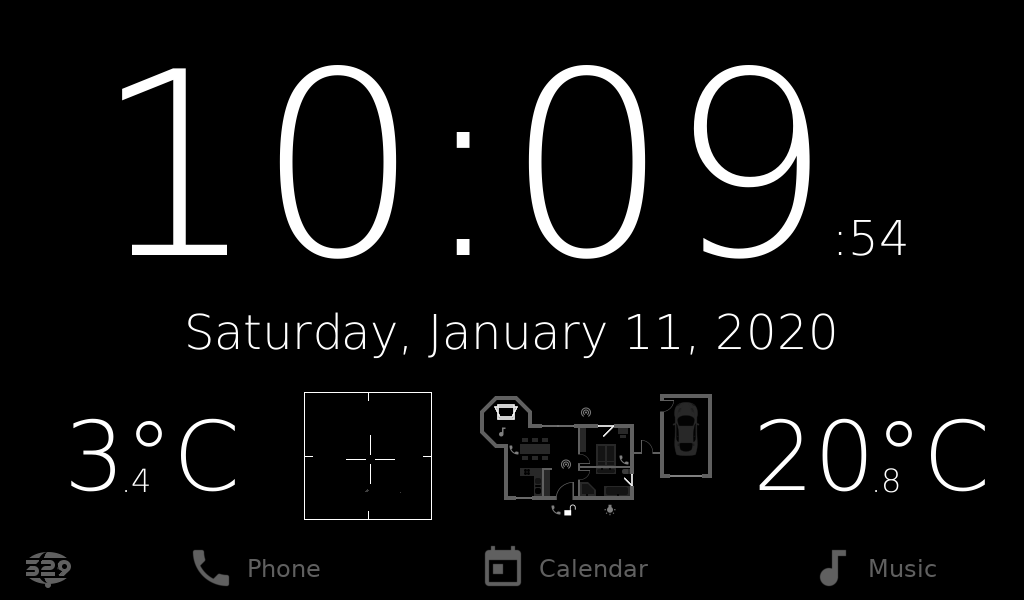
\includegraphics[width=0.7\linewidth]{figs/wallclock-home-2.png}
  \caption[l]{The \textit{WallClock} Main Screen}
  \label{fig:screen-wallclock-home}
\end{figure}


The following functional modules (referred to as \textit{applets}), which are frequently useful in a private household, are integrated in the \textit{WallClock}:

\begin{itemize}
\item
  a SIP-based video phone client (for door phone and inter-room communication),
\item
  a calendar,
\item
  a music player (\textit{MPD} client) designed for a distributed
  setup with many rooms and muktiple user in a household,
\item
  an alarm clock to use the \textit{WallClock} device as a radio alarm clock.
\end{itemize}

Ideally, a \textit{WallClock} device is installed in each room in the house. Due to its resource-aware implementation, low-cost hardware such as cheap or older second-hand Android tablets is sufficient.

The \textit{WallClock} is implemented in native code (C/C++) and uses \textit{SDL2} for its UI. This makes it portable and efficient. So far, the \textit{WallClock} has been tested on (PC) Linux and on Android, but ports of \textit{SDL2} to many other environments exist (see \url{https://libsdl.org}).





%%%%%%%%%%%%%%%%%%%%%%%%%%%%%%%%%%%%%%%%%%%%%%%%%%%%%%%%%%%%%%%%%%%%%%%%%%
\section{The Floor Plan}
\label{sec:wallclock-floorplan}
%%%%%%%%%%%%%%%%%%%%%%%%%%%%%%%%%%%%%%%%%%%%%%%%%%%%%%%%%%%%%%%%%%%%%%%%%%


\subsection{Overview}

The floor plan applet (see Figure~\ref{fig:wallclock-floorplan}) allows to view and to interact with all kinds of gadgets in an intuitive way. Possible gadgets include windows, door locks, garage doors, lights, mailboxes, phones, and motion detectors.

Controllable gadgets can be controlled as shown in Section~\ref{sec:tutorial-firststeps-dialogs}. Shades can be opened and closed by touching their windows, lights and services can be switched on and off. Intercom phone calls can be initiated by pushing the target phone icon.

Depending on the presence state, gadgets can be highlighted to attract the user's attention, if, for example, a window is still open at night or the main door not locked.

The home screen of the \textit{WallClock} shows a mini floor plan, which also shows the states of gadgets (see Figure~\ref{fig:wallclock-minifloorplan}).

\begin{figure}[ht]
  \centering
  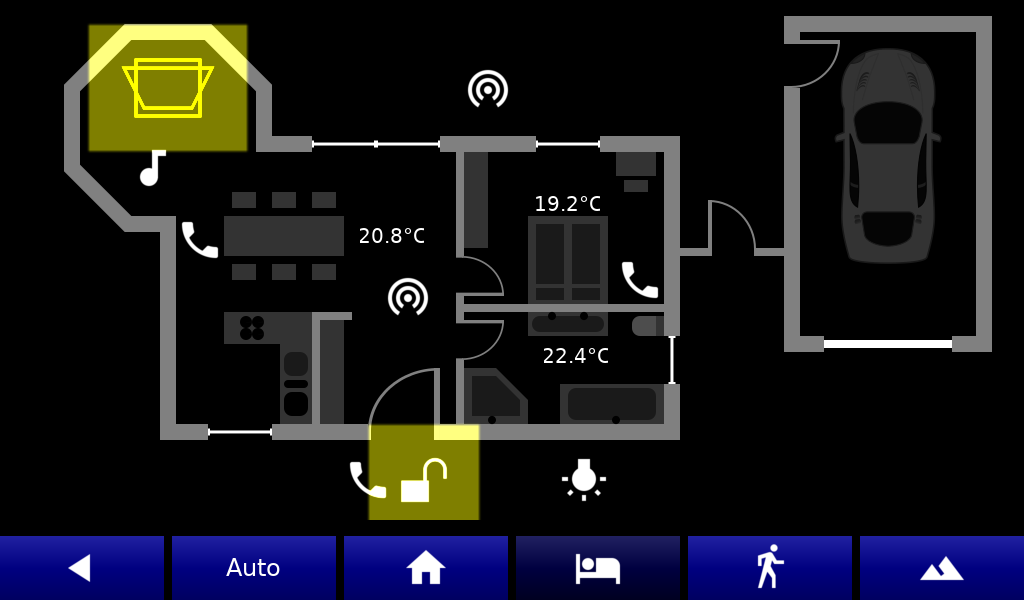
\includegraphics[width=0.7\linewidth]{figs/wallclock-floorplan-4-night.png}
  \caption[l]{The \textit{WallClock} floor plan}
  \label{fig:wallclock-floorplan}
\end{figure}

\begin{figure}[ht]
  \centering
  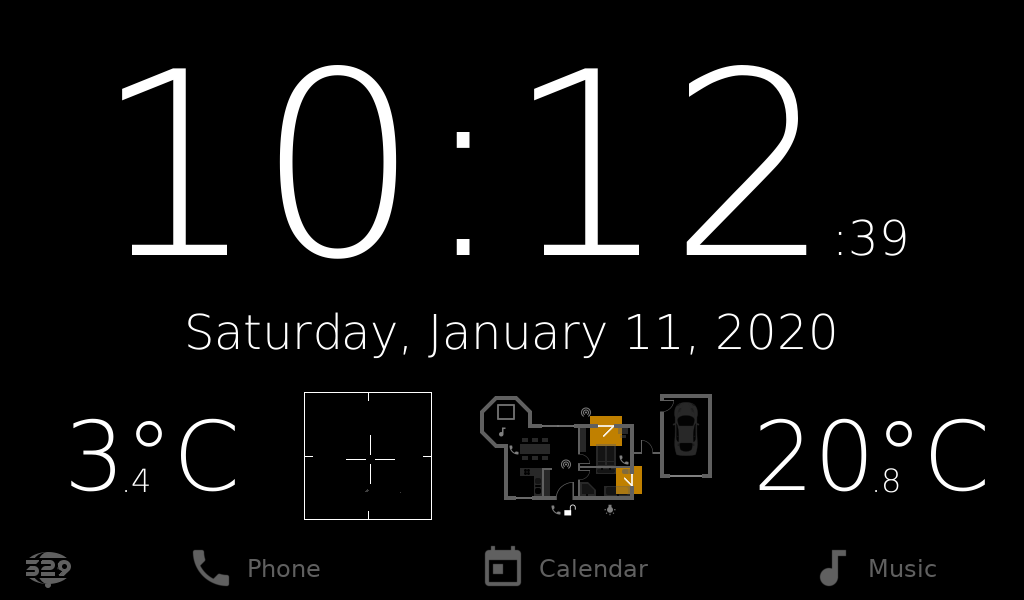
\includegraphics[width=0.7\linewidth]{figs/wallclock-home-5-alert.png}
  \caption[l]{Mini floor plan on the home screen warning about two open windows}
  \label{fig:wallclock-minifloorplan}
\end{figure}


\subsection{Creating a Custom Floor Plan}
\labeltool{home2l-fpc}


The floor plan is specified by an \href{https://en.wikipedia.org/wiki/Scalable_Vector_Graphics}{SVG} drawing and is editable using \href{https://inkscape.org}{Inkscape}, a powerful free drawing tool. A symbol library contains all available gadgets. They can be placed in the drawing, which besides this can be drawn freely.
The \textit{Home2L Floor Plan Compiler} (\reftool{home2l-fpc}) analyses the drawing and creates all necessary data files for the \textit{WallClock} application as well as a template file listing all resources to be used as a template for the \reftool{resources.conf} file.
Gadgets and their resources are identified by their \textit{object IDs} in the SVG drawing.


\subsubsection*{Step 1: Draw the floor plan using \textit{Inkscape}.}

\begin{itemize}
  \item
    The file \refsrc{wallclock/floorplan-template.svg} should be used as a template.
    It also contains a number of hints on how to draw it.
    After a new installation, a copy of this file can usually be found as
    \lstf{\$HOME2L\_ETC/floorplan.svg}. If the file is not at this location: Copy it there.
  \item
    Gadgets are available as a symbol library, which is embedded in the template SVG file.
  \item
    The size of the drawing can be 128x64 or 256x128 pixels, depending on the space
    required for you home.
  \item
    The template has a set of fixed layers. They must not be renamed, reordered or
    removed, but serve certain purposes:
    \begin{description}
      \item[Layer 'helper'] is ignored during compilation and will be invisible.
        It may contain helper material such as a blueprint of the building.
      \item[Layer 'building'] will be rendered as drawn. The contents are arbitrary.
        However, for styling and readability reasons, only grey-level colors should
        be used and all objects should be aligned to pixel boundaries.
      \item[Layer 'gadgets'] contains all gadgets. Refer to the documentation in the
        file for how they may be scaled and rotated.
    \end{description}
\end{itemize}

\subsubsection*{Step 2: Set meaningful IDs for all your gadgets.}

    This can be done using the ''Object Properties'' dialog in \textit{Inkscape}.
    IDs should be lowercase and may contain ''\_'' and ''-'' characters. You are free
    to select your IDs, but it is recommended to use a naming scheme like
    \lst{<room>-<gadget>-<subID>}, for example: \lst{kitchen-shades} or
    \lst{dining-window-l}.

\subsubsection*{Step 3: Compile your SVG file using the floor plan compiler.}
    \begin{lstlisting}[language=bash]
      $ home2l fpc floorplan.svg
    \end{lstlisting}
    This will create a directory \textit{floorplan.fpo} with a number of files directly
    readable by the \textit{WallClock} at run-time. One file,
    \textit{sample-resources.conf} is a template to be used in the next step.
    It contains a list of all resources referred to by the floor plan.

\subsubsection*{Step 4: Update your \reftool{resources.conf} file to assign resources to the floor plan gadgets.}

    Copy the contents of \lst{floorplan.fpo/sample-resources.conf} into your
    \reftool{resources.conf} file and adapt it there. The most relevant part is
    a list of alias definitions. The alias names are generated from your object IDs.
    The alias targets must be adapted to point to the real resources.

    As an aid for testing, a set of local signals are defined and the aliases point to
    them, so that it is possible to test the floor plan in the UI without functionality.

\subsubsection*{Step 5: Copy the floor plan object into the 'etc' directory.}

To activate the floor plan, make sure that the floor plan compiler (\reftool{home2l-fpc})
output resides in \lstf{\$HOME2L\_ETC/floorplan.fpo}.





%%%%%%%%%%%%%%%%%%%%%%%%%%%%%%%%%%%%%%%%%%%%%%%%%%%%%%%%%%%%%%%%%%%%%%%%%%
\clearpage
\section{The Phone}
\label{sec:wallclock-phone}
%%%%%%%%%%%%%%%%%%%%%%%%%%%%%%%%%%%%%%%%%%%%%%%%%%%%%%%%%%%%%%%%%%%%%%%%%%


The \textit{Phone} applet implements a SIP-based VoIP phone with video
fumctionality and the ability to act as a door phone in conjunction
with \reftool{home2l-doorman}. For example, the applet can offer a door
opener button if its peer is a door phone.
Figures~\ref{fig:wallclock-phone-1} and \ref{fig:wallclock-phone-2}
show the phone while ringing and during a video phone call, both in
door phone mode.

Together with a private branch exchange (PBX) software such as
\textit{Asterisk}, the \textit{WallClocks} can be used as an intercom
system for the house and for a sophisticated door phone system with
multiple door bells and multiple answering stations in the building.

In order to compile the \textit{WallClock} with phone capabilities,
\textit{PJSIP} or \textit{Liblinphone} is required.

\begin{figure}[ht]
  \centering
  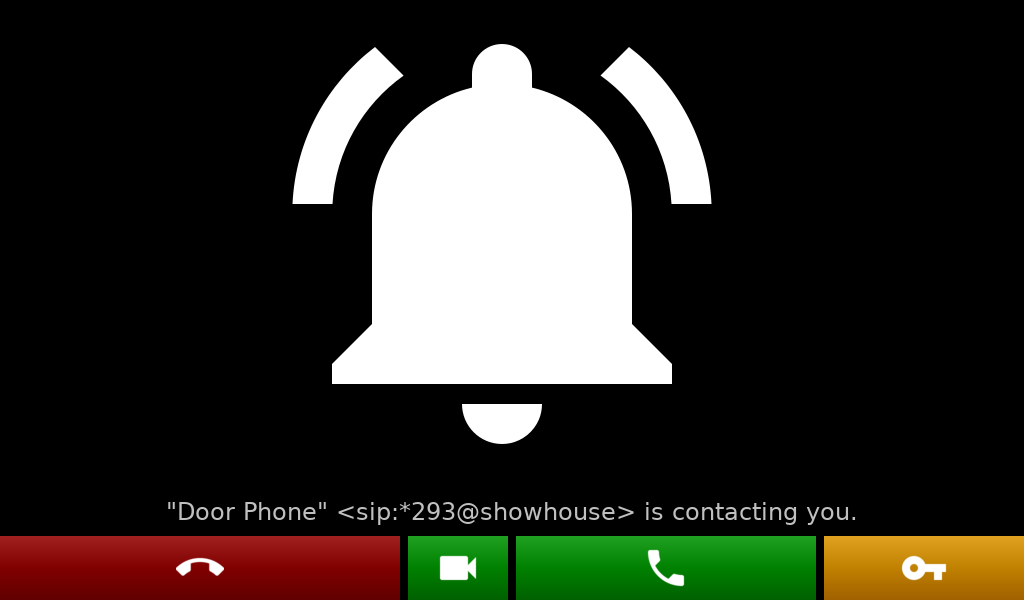
\includegraphics[width=0.7\linewidth]{figs/wallclock-doorman-1.png}
  \caption[l]{The \textit{WallClock} phone: Ringing in door phone mode}
  \label{fig:wallclock-phone-1}
\end{figure}

\begin{figure}[ht]
  \centering
  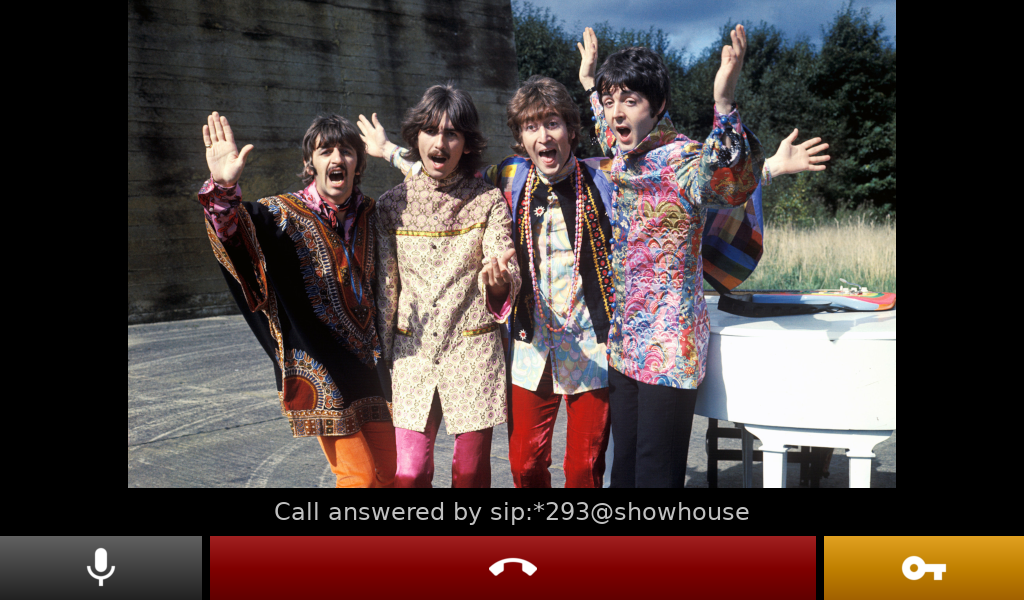
\includegraphics[width=0.7\linewidth]{figs/wallclock-doorman-2.png}
  \caption[l]{
    The \textit{WallClock} phone: Door phone with video\footnotemark[1]
  }
  \label{fig:wallclock-phone-2}
\end{figure}

% NOTE: Check that this footnote is on the same page, not earlier!
\footnotetext[1]{The video image has been created using:
  \url{https://commons.wikimedia.org/wiki/File:TrailerUSHelp.jpg}
}



%%%%%%%%%%%%%%%%%%%%%%%%%%%%%%%%%%%%%%%%%%%%%%%%%%%%%%%%%%%%%%%%%%%%%%%%%%
\section{The Calendar}
\label{sec:wallclock-calendar}
%%%%%%%%%%%%%%%%%%%%%%%%%%%%%%%%%%%%%%%%%%%%%%%%%%%%%%%%%%%%%%%%%%%%%%%%%%


The \textit{Calendar} applet is a graphical calender tool supporting
locally and remotely stored calendars. It supports multiple independent
calendars in a single view, allowing to distinguish private from
business appointments or to manage the activities of multiple family
members (see Figure~\ref{fig:wallclock-calendar}).

\begin{figure}[ht]
  \centering
  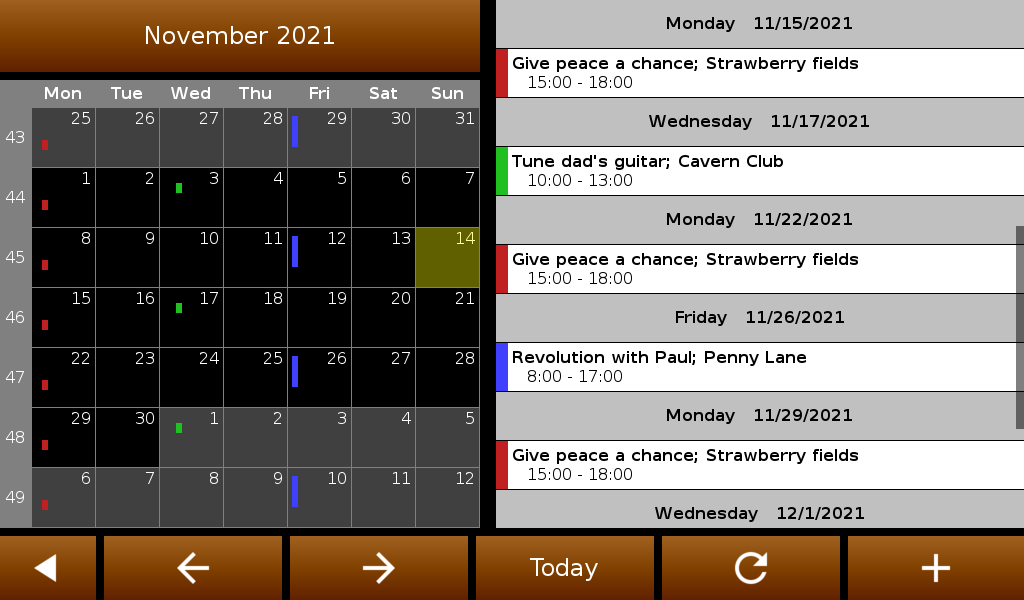
\includegraphics[width=0.7\linewidth]{figs/wallclock-calendar.png}
  \caption[l]{The \textit{WallClock} calendar view}
  \label{fig:wallclock-calendar}
\end{figure}

As its backend and storage format, \textit{remind(1)} is used.
\textit{remind(1)} is a mature and powerful command line tool
supporting single events with and without times as well as
many sorts of recurring events. The main advantage is the fact that a
complete calendar is maintained in one \textit{reminders} file with one
event per line. The file is human-readable and can easily be
edited by hand. Synchonization, merging and even
revision control can easily be accomplished by standard tools such as
\textit{diff(1)}, \textit{meld(1)} and \textit{git(1)}.
Several frontends exist for \textit{remind} (\textit{tkremind(1)}, for example),
the \textit{WallClock Calendar} is a new one with special support for multiple
calendars.

The calendar files can be stored wherever the user likes -- locally or on
a home server.
For any editing operation, \textit{WallClock Calender} generates a \textit{patch(1)}
fragment and passes it to \textit{patch} on the machine storing the calendar file.

This method for accessing calendar files allows a high degree of flexibility
for where and how they are stored, and the use of \textit{patch(1)} supports
concurrent editing operations from multiple \textit{WallClock} instances.

To use the \textit{Calendar} applet, the \textit{remind(1)} command line tool must be installed on some computer reachable by \textit{ssh(1)} by the \textit{WallClock}.



%%%%%%%%%%%%%%%%%%%%%%%%%%%%%%%%%%%%%%%%%%%%%%%%%%%%%%%%%%%%%%%%%%%%%%%%%%
\section{The Music Player}
\label{sec:wallclock-music}
%%%%%%%%%%%%%%%%%%%%%%%%%%%%%%%%%%%%%%%%%%%%%%%%%%%%%%%%%%%%%%%%%%%%%%%%%%


The \textit{WallClock Music Player} is a front end for the
\textit{MPD} music player daemon (\url{https://www.musicpd.org}). It aims to support a home
installations with multiple rooms, multiple users, and multiple virtual or physical
stereo systems. In any room, any user shall be able to control any
stereo system using any \textit{WallClock} device. Everywhere in the house,
he shall have access to the complete music collection and be able to
get it transformed into acoustic air waves by any device he likes:
hifi speakers in the living room, other speakers in the kitchen,
earphones connected to the local device, or bluetooth speakers
coupled with the \textit{WallClock} device. Of course, a user can switch
between them anytime and ''take'' the currently playing music with him as
he moves to another room.

Technically, a ''virtual stereo system'' is an installed \textit{MPD}
instance running on some computer in the household. It has to be
declared in \reftool{home2l.conf} using \refenv{music.<MPD>.host}
and related parameters.

If the \textit{MPDs} are configured with an http streaming output, the
music can be streamed back and played on the local device (\textit{WallClock}
must be compiled with \textit{GStreamer} support for this).

Figure~\ref{fig:screen-wallclock-music} shows a screenshot
with the usual \textit{MPD} controls on the left and a database and
playlist browser on the right. The title bar can be pushed to navigate
up or switch between the local collection and playlists.

\begin{figure}[ht]
  \centering
  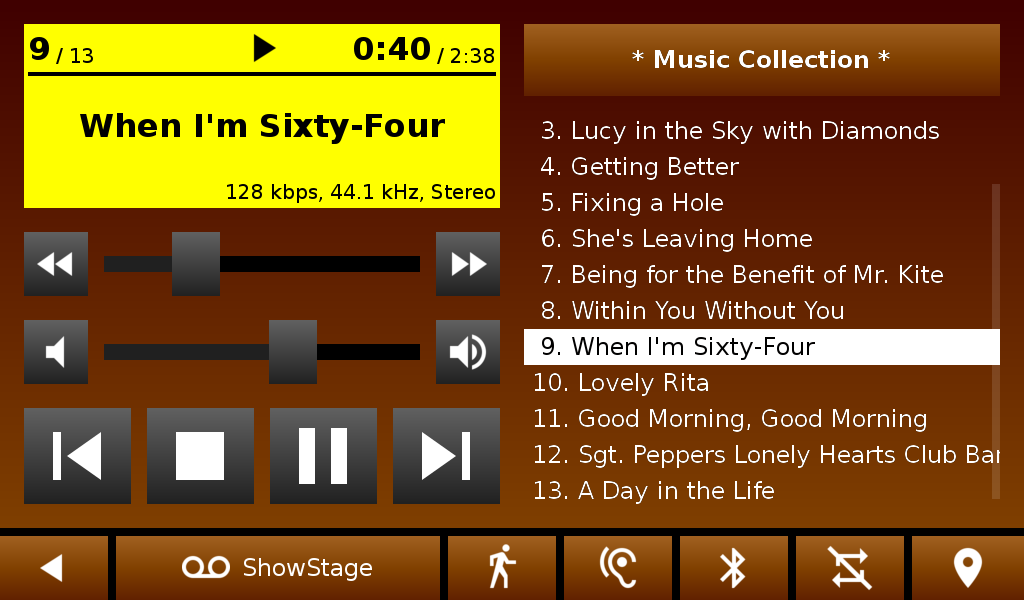
\includegraphics[width=0.7\linewidth]{figs/wallclock-music.png}
  \caption[l]{The \textit{WallClock} Music Player}
  \label{fig:screen-wallclock-music}
\end{figure}

With the buttons in the bottom line you can (from left to right)

\begin{itemize}
\item
  select the ''virtual stereo system'' (\textit{MPD} instance).
\item
  take the currently playing music from one \textit{MPD} instance to another
  (e.g.~to seamlessly continue listening a song when moving from one room to another).
\item
  select the output device (any output configured with \textit{MPD} or
  stream to the local device, if available).
\item
  enable or disable Bluetooth (Android).
\item
  select the repeat mode.
\item
  navigate to the currently playing song.
\end{itemize}

The \refrc{ui/mute} resource allows to mute the music player by automation
rules, for example, if the phone rings.

A long push on the ''Music'' launcher on the main screen (Figure~\ref{fig:screen-wallclock-home})
turns the music player on or off without switching to the music screen.



%%%%%%%%%%%%%%%%%%%%%%%%%%%%%%%%%%%%%%%%%%%%%%%%%%%%%%%%%%%%%%%%%%%%%%%%%%
\section{The Alarm Clock}
\label{sec:wallclock-alarmclock}
%%%%%%%%%%%%%%%%%%%%%%%%%%%%%%%%%%%%%%%%%%%%%%%%%%%%%%%%%%%%%%%%%%%%%%%%%%

The alarm clock can be enabled by pushing the clock display on the main screen.
For each weekday, an individual alarm time can be programmed.

By default, the music player is activated on alarm. If the music player fails
or the music is not loud enough (see \refenv{alarm.minLevelDb}), a ringing
sound is played as a fallback.

For the case that the alarm clock fails completely, a dead-man script can
be submitted to another computer, which can then wake you up with some
other means (e.g.~by a wakeup call to your mobile phone).
See \refenv{alarm.extAlarmHost}, \refenv{alarm.extAlarmCmd} and \refenv{alarm.extAlarmDelay}
for details.



%%%%%%%%%%%%%%%%%%%%%%%%%%%%%%%%%%%%%%%%%%%%%%%%%%%%%%%%%%%%%%%%%%%%%%%%%%
\section{List of Configuration Parameters}
\label{sec:wallclock-env}
%%%%%%%%%%%%%%%%%%%%%%%%%%%%%%%%%%%%%%%%%%%%%%%%%%%%%%%%%%%%%%%%%%%%%%%%%%

\input{ref_env_wallclock}



%%%%%%%%%%%%%%%%%%%%%%%%%%%%%%%%%%%%%%%%%%%%%%%%%%%%%%%%%%%%%%%%%%%%%%%%%%
\section{List of Provided Resources}
\label{sec:wallclock-rc}
%%%%%%%%%%%%%%%%%%%%%%%%%%%%%%%%%%%%%%%%%%%%%%%%%%%%%%%%%%%%%%%%%%%%%%%%%%

\input{ref_rc_wallclock}





%%%%%%%%%%%%%%%%%%%%%%%%%%%%%%%%%%%%%%%%%%%%%%%%%%%%%%%%%%%%%%%%%%%%%%%%%%%%%%%
%
\chapter{\textit{DoorMan} -- A Doorbell and Doorphone Service}
\label{ch:doorman} \labeltool{home2l-doorman}
%
%%%%%%%%%%%%%%%%%%%%%%%%%%%%%%%%%%%%%%%%%%%%%%%%%%%%%%%%%%%%%%%%%%%%%%%%%%%%%%%


\section{Overview}
\label{sec:doorman-overview}

\textit{DoorMan} is a doorbell and doorphone service operated on the
command line or as a background service. It must be linked with an IP
phone library (\textit{PJSIP} or \textit{Liblinphone}).





%%%%%%%%%%%%%%%%%%%%%%%%%%%%%%%%%%%%%%%%%%%%%%%%%%%%%%%%%%%%%%%%%%%%%%%%%%
\section{List of Configuration Parameters}
\label{sec:doorman-env}
%%%%%%%%%%%%%%%%%%%%%%%%%%%%%%%%%%%%%%%%%%%%%%%%%%%%%%%%%%%%%%%%%%%%%%%%%%

\input{ref_env_doorman}


%%%%%%%%%%%%%%%%%%%%%%%%%%%%%%%%%%%%%%%%%%%%%%%%%%%%%%%%%%%%%%%%%%%%%%%%%%
\section{List of Provided Resources}
\label{sec:doorman-rc}
%%%%%%%%%%%%%%%%%%%%%%%%%%%%%%%%%%%%%%%%%%%%%%%%%%%%%%%%%%%%%%%%%%%%%%%%%%

\input{ref_rc_doorman}





%%%%%%%%%%%%%%%%%%%%%%%%%%%%%%%%%%%%%%%%%%%%%%%%%%%%%%%%%%%%%%%%%%%%%%%%%%
%
\chapter{Driver Library}
\label{ch:drvlib}
%
%%%%%%%%%%%%%%%%%%%%%%%%%%%%%%%%%%%%%%%%%%%%%%%%%%%%%%%%%%%%%%%%%%%%%%%%%%


This chapter is the reference documentation of all supplied drivers.





%%%%%%%%%%%%%%%%%%%%%%%%%%%%%%%%%%%%%%%%%%%%%%%%%%%%%%%%%%%%%%%%
\section{The \textit{Signal} Driver (built-in)}
\label{sec:drvlib-signal} \labeltool{home2l-drv-signal}
%%%%%%%%%%%%%%%%%%%%%%%%%%%%%%%%%%%%%%%%%%%%%%%%%%%%%%%%%%%%%%%%


The \textit{Signal} driver is always available and allows to declare resources
which just report back any driven value without any technical functionality.

Signals can serve as intermediate resources or for testing purposes.

They can be defined inside a \reftool{resources.conf} configuration file
(see Section~\ref{sec:resources-conf-signals}) or by the API calls
\refapic{RcRegisterSignal()} (C/C++) or \refapipython{NewSignal()} (Python).





%%%%%%%%%%%%%%%%%%%%%%%%%%%%%%%%%%%%%%%%%%%%%%%%%%%%%%%%%%%%%%%%
\section{The \textit{Timer} Driver (built-in)}
\label{sec:drvlib-timer} \labeltool{home2l-drv-timer}
%%%%%%%%%%%%%%%%%%%%%%%%%%%%%%%%%%%%%%%%%%%%%%%%%%%%%%%%%%%%%%%%


\subsection{Description}
\label{sec:drvlib-timer-description}

The driver \textit{timer} provides resources reflecting the current time, triggers to initiate hourly or daily tasks, and a set of resources reflecting day and night times, suitable, for example, to control an automatic outdoor light.

The driver is statically built into the \textit{Resources} library and enabled by default. It can be disabled by the \refenv{rc.timer} setting.


\subsection{Provided Resources}
\label{sec:drvlib-timer-rc}

\input{ref_rc_resources}





%%%%%%%%%%%%%%%%%%%%%%%%%%%%%%%%%%%%%%%%%%%%%%%%%%%%%%%%%%%%%%%%%%%%%%%%%%
\section{The \textit{GPIO} Driver}
\label{sec:drvlib-gpio} \labeltool{home2l-drv-gpio}
%%%%%%%%%%%%%%%%%%%%%%%%%%%%%%%%%%%%%%%%%%%%%%%%%%%%%%%%%%%%%%%%%%%%%%%%%%


\subsection{Description}
\label{sec:drvlib-gpio-description}

The driver \textit{gpio} is a universal driver leveraging the Linux \textit{sysfs} GPIO capabilities to access general purpose inputs and outputs (GPIO).

In order to allow GPIOs to be used from a normal user application, they must be set up properly beforehand. This preparation requires \textit{root} privileges and is therefore done by the \textit{Home2L} init script at boot time. The names and configurations (e.~g. direction, initial value) of available GPIOs are defined by symbolic links residing in
\begin{lstlisting}
  $HOME2L_ETC/gpio.<machine name>
\end{lstlisting}

pointing to the actual device, typically:
\begin{lstlisting}
  /sys/class/gpio/gpio<n>
\end{lstlisting}

The links are read both by the \textit{GPIO} driver and the init script,
and they must conform to the following naming conventions:
\begin{lstlisting}
$HOME2L_ETC/gpio.<machine name>/<port name>.<options>

<options> is a sequence of characters and may include:
    i - The port is an input.
    0 - The port is an output with a default value of 0.
    1 - The port is an output with a default value of 1.
    n - The port is active-low (negated).
\end{lstlisting}


%\subsection{Configuration Parameters}
%\label{sec:drvlib-gpio-env}
%\input{ref_env_drv_gpio}
%
% ! The configuration may in the future move to 'home2l.conf'.
% ! Then the previous lines have to be commented in.


\subsection{Provided Resources}
\label{sec:drvlib-gpio-rc}

The provided resources depend on the configuration (see above).
They are named after their port names (\textit{gpio/<port name>})
as specified in the name of the symbolic link.





%%%%%%%%%%%%%%%%%%%%%%%%%%%%%%%%%%%%%%%%%%%%%%%%%%%%%%%%%%%%%%%%%%%%%%%%%%
\section{The \textit{MQTT} Gateway Driver}
\label{sec:drvlib-mqtt} \labeltool{home2l-drv-mqtt}
%%%%%%%%%%%%%%%%%%%%%%%%%%%%%%%%%%%%%%%%%%%%%%%%%%%%%%%%%%%%%%%%%%%%%%%%%%


\subsection{Description}
\label{sec:drvlib-mqtt-description}

The MQTT gateway driver (\reftool{home2l-drv-mqtt}) allows to interconnect a \textit{Home2L} cluster with an MQTT network. Strictly speaking, it is not just driver, but actually performs two task:
\begin{enumerate}[a)]
  \item It can \textit{import} arbitrary resources from the MQTT network and make them available as \textit{Home2L} resources (this is the driver functionality).
  \item It can \textit{export} \textit{Home2L} resources to the MQTT network in order to make them available to external visualization tools or other home automation frameworks, for example.
\end{enumerate}

Figure~\ref{fig:mqtt-topology} sketches an example topology an the role of the MQTT gateway driver.
The gateway driver can export and import resources of and and for the complete \textit{Home2L} cluster and may be hosted by any of the instances at the administrator's choice. It is also possible to run multiple instances of the driver in multiple \textit{Home2L} instances, for example, in order to communicate with multiple brokers.

Towards the MQTT broker, the gateway driver acts like an MQTT client.

\begin{figure}[ht]
  \centering
  \figsvg[width=0.9\linewidth]{figs/mqtt-topology.svg}
  \caption[l]{Example topology of a \textit{Home2L} cluster and an MQTT broker/client network}
  \label{fig:mqtt-topology}
\end{figure}

%Section~\ref{sec:drvlib-mqtt-background} gives some background information for understanding how messages are translated between the \textit{Home2L} and the MQTT domain. Sections~\ref{sec:drvlib-mqtt-importing} and \ref{sec:drvlib-mqtt-exporting} contain instructions and examples on importing MQTT devices and exporting \textit{Home2L} resources, respectively. Section~\ref{drvlib-mqtt-details} contain some specific details related to the MQTT protocol and the client implementation of the driver.



%\subsection{}
%\label{sec:drvlib-mqtt-background}

Actually, the communication of \textit{Home2L} instances and the MQTT protocol are very similar:
\begin{itemize}
  \item Both use a publish-subscribe pattern for communication.
  \item There is a hierarchical name space for identifying resources (\textit{Home2L} URIs and MQTT topics, respectively).
    The syntax is very similar.
\end{itemize}

But there are also some differences:

\begin{itemize}

  \item
    \textit{Home2L Resources} is object-oriented, whereas MQTT is message-oriented. \textit{Home2L Resources}
    specifies an API, wheras MQTT specifies a protocol. The \textit{Home2L Resources} library offers API methods to
    obtain and manipulate both the value and state of \refapic{CResource} objects. It keeps track of the state and
    validity of an object (= resource) and coordinates manipulation requests to it. A resource is identified by a single
    URI.

    Different from this, MQTT-enabled devices typically use multiple different topics per physical resource for
    state reporting, manipulation and reporting of its validity.

  \item
    The MQTT protocol has no equivalent to the \textit{Home2L} request resolution mechanism. With MQTT, concurrent
    manipulations must be coordinated at the application level.

  \item
    \textit{Home2L} resources are typed, MQTT payloads are not.

  \item
    With MQTT, all messages are sent to and received from a central broker, whereas \textit{Home2L} instances
    communicate directly.

\end{itemize}

These differences should be kept in mind when configuring the gateway driver.



\subsection{Importing External Resources from the MQTT Broker}
\label{sec:drvlib-mqtt-importing}

External resources are imported by a single-line \refenv{mqtt.import.<ID>} entry in the \reftool{home2l.conf} file.

Up to three different topics can be specified for a resource:
\begin{itemize}
  \item the \textit{state} topic for reporting the current state,
  \item the \textit{request} topic (also known as the \textit{command} topic) for manipulations,
  \item the \textit{validity} topic (sometimes called the \textit{alive} topic) for indicating whether the client
      is currently alive and a connection to the broker exists.
\end{itemize}

Messages to the state topic are reported as valid values for the respective resource. If a message for the validity indicates that the client is offline, a state of \refapic{rcsUnknown} is reported.

Whenever the set of active requests indicates that a new value has to be driven (see Figure~\ref{fig:resources-terminology}), the gateway sends a message with the new value on the request topic.

The correct settings for an \refenv{mqtt.import.<ID>} entry can be found in the documentation of the respective device or determined by monitoring MQTT messages with:
\begin{lstlisting}[language=bash]
  $ mosquitto_sub [-t <broker>] -v -t '#'
\end{lstlisting}
The tool \textit{mosquitto\_sub} is part of the \href{https://mosquitto.org}{Mosquitto} project.



\subsection{Exporting \textit{Home2L} Resources to the MQTT Broker}
\label{sec:drvlib-mqtt-exporting}

Each \textit{Home2L} resource can be exported by a single-line \refenv{mqtt.export.<ID>} entry in the \reftool{home2l.conf} file. Alternatively, multiple resources can be exported with a single \refenv{mqtt.exportSet}
entry. However, the latter variant has some restrictions and is thus only recommended for testing purposes.

For each exported resource, the \textit{state} topic and optionally the \textit{request} (aka \textit{command})
topic can be specified.

Values are published as UTF-8 strings with the \textit{Home2L} syntax, which should be acceptable by most devices and other MQTT clients. For Boolean resources, the strings sent for the values ''false'' and ''true'' can be specified explicitly with the \refenv{mqtt.export.<ID>} setting.
Unknown values or values of state \refapic{rcsBusy} are published with the \textit{Home2L} syntax (''?'' or with a ''!'' prefix, respectively). This behavior can be adjusted with the \refenv{mqtt.unknownSign} and \refenv{mqtt.busySign} settings.

Messages received for the request topic originating from some other MQTT client are automatically transformed
into a \textit{Home2L} request. The attributes of such requests can be adjusted by the \refenv{mqtt.reqId} and \refenv{mqtt.reqAttrs} settings.



\subsection{Background Information}
\label{sec:drvlib-mqtt-details}

The currently supported protocol versions are MQTT version 3.1 / 3.1.1.

The driver always connects in ''clean session'' mode (no persistent session).

The driver opens a single session for all imports and exports. Sometimes, multiple sessions for different \textit{Home2L} resources may be desired, for example, to connect with multiple different brokers. This can be implemented by running multiple \textit{Home2L} instances, each of which exporting or importing a subset of resources.

All messages sent by the driver are sent as retained messages, and they are cleared when the driver is stopped properly. Adversely, \textit{state} messages for imported resources should be sent as retained messages by their sender. Devices should be configured to send retained messages.

Some considerations on selecting the QoS level, which can be set by the \refenv{mqtt.qos} option:
\begin{itemize}
  \item For the common case of a TCP network connection to the broker, QoS level 0
      may be sufficient, since TCP itself implements a reliable transmission.
  \item The \textit{Home2L Resources} library can tolerate duplicated messages. However, it implements strict event
      ordering and relies on the correct ordering of messages. For this reason, QoS level 1 should not be used.
      According to the MQTT 3.1.1 specification, it may happen that a re-send of an earlier message
      is received after its successor message unless the client explicitly waits for the earlier message
      to be acknowledged before sending the next message. Such a behavior is not implemented in this driver.
  \item With an unreliable connection to the broker, QoS level 2 should be considered.
\end{itemize}



\subsection{Configuration Parameters}
\label{sec:drvlib-mqtt-env}
\input{ref_env_drv_mqtt}



\subsection{Provided Resources}

The set of provided resources is controlled by the \refenv{mqtt.import.<ID>} settings.





%%%%%%%%%%%%%%%%%%%%%%%%%%%%%%%%%%%%%%%%%%%%%%%%%%%%%%%%%%%%%%%%%%%%%%%%%%
\section{The \textit{Brownies} Driver}
\label{sec:drvlib-brownies} \labeltool{home2l-drv-brownies}
%%%%%%%%%%%%%%%%%%%%%%%%%%%%%%%%%%%%%%%%%%%%%%%%%%%%%%%%%%%%%%%%%%%%%%%%%%


\subsection{Description}
\label{sec:drvlib-brownies-description}

The \textit{Brownies} driver is a universal driver continuously polling a \textit{Brownie} bus tree and exporting resources for all features of all \textit{Brownies} declared in the database.

For its operation, a database (\reftool{brownies.conf}) is required, which defines the set of \textit{Brownies} to be polled. Devices without a valid and consistent database entry are ignored by the driver. Details on creating, updating and verifying the database can be found in Section~\ref{sec:brownies-database}.

The driver supports a single \textit{Brownie} tree associated with a single \textit{i2c} root master interface of the host machine. Multiple trees connected to the same Linux machine via multiple \textit{i2c} interfaces can be driven by running separate \textit{Home2L} instances for each interface, each running an instance of this driver with an individual database file.

Note: This driver cannot be hosted by \reftool{home2l-brownie2l}, which contains its own built-in version of a \textit{Brownie} driver.


\subsection{Configuration Parameters}
\label{sec:drvlib-brownies-env}
\input{ref_env_brownies}


\subsection{Provided Resources}
\label{sec:drvlib-brownies-rc}
\input{ref_rc_brownies}





%%%%%%%%%%%%%%%%%%%%%%%%%%%%%%%%%%%%%%%%%%%%%%%%%%%%%%%%%%%%%%%%%%%%%%%%%%
\section{The \textit{EnOcean} Driver}
\label{sec:drvlib-enocean} \labeltool{home2l-drv-enocean}
%%%%%%%%%%%%%%%%%%%%%%%%%%%%%%%%%%%%%%%%%%%%%%%%%%%%%%%%%%%%%%%%%%%%%%%%%%


\subsection{Description}
\label{sec:drvlib-enocean-description}

The \textit{EnOcean} driver allows to import energy harvesting sensors using the \textit{EnOcean} radio protocol over a \textit{USB 300 / TCM 310} gateway module.

The set of supported devices includes push buttons and mechanical window handles. The \textit{WallClock} floor plan applet can combine window state sensors together with window handle data to, for example, visualize whether a closed patio door is locked or still unlocked (handle in the "open" position).

A complete list together with their \textit{EnOcean Equippment Profile (EPP)} identifiers can be found in \refsrc{drivers/enocean/home2l-drv-enocean.C} in section \textit{Equipment Drivers}. Support for new equipment profiles can be added there.



\subsection{Importing \textit{EnOcean} Devices}
\label{sec:drvlib-enocean-importing}
\labeltool{home2l-enocean2l}

Devices are imported by a single-line \refenv{enocean.device.<ID>} entry in the \reftool{home2l.conf} file. The device ID and profile can usually be found in the device configuration.

To determine the device ID and for testing, the tool \reftool{home2l-enocean2l} can be used. It displays all radio telegrams received together with the signal strength:
\begin{lstlisting}[language=bash]
  $ home2l enocean2l enocean.link=/dev/ttyUSB1
  home2l-enocean2l v1.1-92-g02cc (2020-09-05) by Gundolf Kiefer

  Waiting for EnOcean telegrams on '/dev/ttyUSB1' ...
  : DevID=0517fca6 RORG=f6 Data=e0 Status=20 dBm=61
  : DevID=0517fca6 RORG=f6 Data=f0 Status=20 dBm=58
  ...

\end{lstlisting}



\subsection{Configuration Parameters}
\label{sec:drvlib-enocean-env}
\input{ref_env_drv_enocean}



\subsection{Provided Resources}

The set of provided resources is controlled by the \refenv{enocean.device.<ID>} settings.






%%%%%%%%%%%%%%%%%%%%%%%%%%%%%%%%%%%%%%%%%%%%%%%%%%%%%%%%%%%%%%%%%%%%%%%%%%
\section{The \textit{Weather} Driver}
\label{sec:drvlib-weather} \labeltool{home2l-drv-weather}
%%%%%%%%%%%%%%%%%%%%%%%%%%%%%%%%%%%%%%%%%%%%%%%%%%%%%%%%%%%%%%%%%%%%%%%%%%


\subsection{Description}
\label{sec:drvlib-weather-description}

The \textit{Weather} driver provides local weather information by querying
the \href{https://opendata.dwd.de}{Open Data} service of the German Weather
Service (DWD).


\subsection{Configuration Parameters}
\label{sec:drvlib-weather-env}
\input{ref_env_drv_weather}


\subsection{Provided Resources}
\label{sec:drvlib-weather-rc}
\input{ref_rc_drv_weather}





%%%%%%%%%%%%%%%%%%%%%%%%%%%%%%%%%%%%%%%%%%%%%%%%%%%%%%%%%%%%%%%%%%%%%%%%%%
\section{The \textit{MPD} Monitor Driver}
\label{sec:drvlib-mpd} \labeltool{home2l-drv-mpd}
%%%%%%%%%%%%%%%%%%%%%%%%%%%%%%%%%%%%%%%%%%%%%%%%%%%%%%%%%%%%%%%%%%%%%%%%%%


\subsection{Description}
\label{sec:drvlib-mpd-description}

The \textit{MPD} monitor driver connects to running MPD instances and provides their player states as resources of type \refapic{ERctPlayerState}.

Also, MPD players being in a paused state for a longer time are stopped after a defined time.



\subsection{Configuration Parameters}
\label{sec:drvlib-mpd-env}
\input{ref_env_drv_mpd}


\subsection{Provided Resources}
\label{sec:drvlib-mpd-rc}

For each defined MPD server, a read-only resource of type \refapic{ERctPlayerState} is provided with the local ID (LID) being equal to the server ID.





%%%%%%%%%%%%%%%%%%%%%%%%%%%%%%%%%%%%%%%%%%%%%%%%%%%%%%%%%%%%%%%%%%%%%%%%%%%%%%%
%                                                                             %
%                             Appendix                                        %
%                                                                             %
%%%%%%%%%%%%%%%%%%%%%%%%%%%%%%%%%%%%%%%%%%%%%%%%%%%%%%%%%%%%%%%%%%%%%%%%%%%%%%%


\appendix





%%%%%%%%%%%%%%%%%%%%%%%%%%%%%%%%%%%%%%%%%%%%%%%%%%%%%%%%%%%%%%%%%%%%%%%%%%%%%%%
%
\chapter{Appendix: Documentation How-To}
%
%%%%%%%%%%%%%%%%%%%%%%%%%%%%%%%%%%%%%%%%%%%%%%%%%%%%%%%%%%%%%%%%%%%%%%%%%%%%%%%



%%%%%%%%%%%%%%%%%%%%%%%%%%%%%%%%%%%%%%%%%%%%%%%%%%%%%%%%%%%%%%%%%%%%%%%%%%
\section{Writing the \textit{Home2L Book}}
\label{sec:documenting-the_book}
%%%%%%%%%%%%%%%%%%%%%%%%%%%%%%%%%%%%%%%%%%%%%%%%%%%%%%%%%%%%%%%%%%%%%%%%%%


\subsection{Formatting}

\begin{description}
  \item[\lst{\code{foo_bar}}] ~ \\
    Print as code, not specially highlighted, but '\_' characters are allowed without escaping.
    \textit{Note: Spaces are not allowed in the text!}
  \item[\lst{\lst{foo_bar}}] ~ \\
    Inline listing, with the rules of \code{\code{}} applied.
    \textit{Note: Spaces are not allowed in the text!}
  \item[\lst{\lstf{foobar}}] ~ \\
    Inline listing formattable. LaTeX formatting is allowed, but '\_' characters must be escaped,
    for example.
  \item[\lst{\begin{lstlisting}} ... \lst{\end{lstlisting}}] ~ \\
    Display listing: full text witdh, with auto-wrapping. The following languages are supported
    (\lst{\begin{lstlisting}[language=<language>]}):
    \begin{description}
      \item[(default):] Plain, all text black.
      \item[comments:] All text black, only comments starting with \lst{#} are grey.
      \item[bash:] Bash session: Lines starting with \lst{\$ } (commands) black, output and
         comments grey. Command lines can be prefixed with ''§'' explicitly.
      \item[python:] Python session: Lines starting with \lst{>>> } (commands) black, output and
         comments grey. Command lines can be prefixed with ''§'' explicitly.
      \item[home2l:] \reftool{home2l-shell} session: Commands black, output grey.
      \item[brownie2l:] \reftool{home2l-brownie2l} session: Commands black, output grey.
    \end{description}
  \item[\lst{\lstbox{foobar}}] ~ \\
    Display listing, for places where the former are not allowed, e.~g. in info boxes
\end{description}



\subsection{Info and Warn Boxes}

\begin{description}
  \item[\lstf{\\infobox\{multi-line text\}}] ~ \\
    Print an info box. Info boxes contain supplemental information, not required for all readers.
  \item[\lstf{\\warnbox\{multi-line text\}}] ~ \\
    Print a warn box. Such boxes contain important information, requiring special attention from
    the reader.
\end{description}



\subsection{Internal References: Tools, Configuration, Resources}

\subsubsection{Labeling}
\begin{description}
  \item[\lst{\labeltool{home2l-newtool}}] ~ \\
    Set section label to define a new tool.
  \item[\lst{\idx{term}}] ~ \\
    Add and link word ''term'' to the index, while printing it as-is in the text.
\end{description}

\subsubsection{Referencing}
\begin{description}
  \item[\lst{\reftool{home2l-sometool}}] ~ \\
    Reference a tool.
  \item[\lst{\refenv{domain.some.variable}}] ~ \\
    Reference the environment parameter \code{domain.some.variable}.
  \item[\lst{\refrc{driver/local/id}}] ~ \\
    Reference a resource by its host-local ID.
\end{description}



% External references (Doxygen and sources) ...
\subsection{External References: Source files, Doxygen Pages, Internet}
\begin{description}
  \item[\lst{\refdoc{path/to/file}{written_text}}] ~ \\
    Add a hyperlink to some document in the source tree. The file name is given relative to the source tree.
    The ''written text'' appears without special formatting. Typical use: Referencing some other
    PDF document such as \code{README.pdf} or some Doxygen HTML document.
  \item[\lst{\refsrc{path/to/file}}] ~ \\
    Add a hyperlink to some source file. The filename is written in typewriter font.
  \item[\lst{\href{url}{written_text}}] ~ \\
    Add a hyperlink to some internet URL.

  \item[\lst{\refapic{name}}] ~ \\
    Add a reference to some C/C++ class, function, or other type of declaration.
    Presently, this prints the name of the object (''\code{name}'') and links it to the main
    page of the C/C++ API. The name can be entered into the ''search'' field of the Doxygen internal
    search.
  \item[\lst{\refapicgroup{group__subgroup}{code_documentation_(group/subgroup)}}] ~ \\
    Add a reference to a Doxygen group in the C/C++ API as declared by '@newgroup'.
    The second argument is an example for the written text.
    \\ \textbf{Note:} Underscores must be doubled in the first argument!
  \item[\lst{\theapic{}}] ~ \\
    Print the text ''C/C++ API'' with a hyperlink to the main page of the C/C++ API documentation.

  \item[\lst{\refapipython{name}}] ~ \\
    Add a reference to some Python function or other type of declaration.
    Presently, this prints the name of the object (''\code{name}'') and links it to the main
    page of the Python API. The name can be entered into the ''search'' field of the Doxygen internal
    search.
  \item[\lst{\refapipythongroup{group__subgroup}{code_documentation_(group/subgroup)}}] ~ \\
    Add a reference to a Doxygen group in the Python API as declared by '@newgroup'.
    The second argument is an example for the written text.
    \\ \textbf{Note:} Underscores must be doubled in the first argument!
  \item[\lst{\theapipython{}}] ~ \\
    Print the text ''Python API'' with a hyperlink to the main page of the Python API documentation.
\end{description}



%%%%%%%%%%%%%%%%%%%%%%%%%%%%%%%%%%%%%%%%%%%%%%%%%%%%%%%%%%%%%%%%%%%%%%%%%%
\section{Documenting Configuration Parameters}
%%%%%%%%%%%%%%%%%%%%%%%%%%%%%%%%%%%%%%%%%%%%%%%%%%%%%%%%%%%%%%%%%%%%%%%%%%

Configuration parameters are documented by means of a specially formatted comment following the respective
\refapicgroup{env__declaration}{\code{ENV_PARA_...}} macro defined in \refsrc{common/env.H}. The comment has the following structure:
\begin{lstlisting}
ENV_PARA_... (...);
  /* Short description (max. ~40 chars, no trailing period)
   *
   * Optional long description, optionally covering multiple lines or empty lines.
   * Only the last line must not be empty, and there must be exactly one empty
   * line between the short and the long description.
   *
   * Formatting can be done with LaTeX syntax.
   */
\end{lstlisting}

In the description part, any formatting or cross-referencing macros described in Section~\ref{sec:documenting-the_book}
can be used.



%%%%%%%%%%%%%%%%%%%%%%%%%%%%%%%%%%%%%%%%%%%%%%%%%%%%%%%%%%%%%%%%%%%%%%%%%%
\section{Documenting Resources}
%%%%%%%%%%%%%%%%%%%%%%%%%%%%%%%%%%%%%%%%%%%%%%%%%%%%%%%%%%%%%%%%%%%%%%%%%%


Resources are documented by special comments following the respective \refapic{RcRegisterResource()},
\refapic{CResource::Register()}, or \refapic{CRcDriver::RegisterResource()} invocations:
\begin{lstlisting}
rcMyFirst = RcRegisterResource (drv, "myFirstLid", rctBool, false);
  /* [RC:mydriver] Some read-only Boolean resource
   */
\end{lstlisting}
\begin{lstlisting}
rcMySecond = drv->RegisterResource ("mySecondLid", rctPercent, true);
rcMySecond->SetDefault (0.0);
  /* [RC:mydriver] Some writable resource with a percentage value type and a default request
   *
   * Optional long description, optionally covering multiple lines or empty lines.
   * Only the last line must not be empty, and there must be exactly one empty
   * line between the short and the long description.
   *
   * Formatting can be done with LaTeX syntax.
   */
\end{lstlisting}


The following conditions must be met:
\begin{itemize}
  \item If a default value is to be set, the respective \refapic{SetDefault()} call must follow the registering call in the
      next line.
  \item The next line must be a comment of the form \lstf{/* [RC:<driver>] <brief description>}.
  \item The \lstf{[RC:<driver>]} clause defines the driver.
  \item Other information -- the Resource's local ID (LID), its type, an the writability flag are extracted from the registering
      call. If the LID and/or default value are not written explicitely in these lines (e.g. they are calculated in variables),
      they can be appended to the \code{[RC]} clause: \lst{[RC:<driver>:<lid>]...} or \lst{[RC:<driver>:<lid>:<default>]...}. Examples can be found in \refsrc{brownies/brownies.C}.
  \item The comment block must end with a line starting with ''*/'' (end of comment).
  \item To explicitly exclude the resource from documentation, place a line with \lstf{/* [RC:-] */} behind the registering
      call (either in the same or the following line).
\end{itemize}

The following characters are automatically escaped and may appear without escaping in the text:
\texttt{'\_', '\#', '\$', '\%'}.

As for the documentation of configuration parameters, the short description has no trailing period, and in the description part, any formatting or cross-referencing macros described in Section~\ref{sec:documenting-the_book} can be used.




%%%%%%%%%%%%%%%%%%%%%%%%%%%%%%%%%%%%%%%%%%%%%%%%%%%%%%%%%%%%%%%%%%%%%%%%%%
\section{Doxygen Cheat Sheet}
%%%%%%%%%%%%%%%%%%%%%%%%%%%%%%%%%%%%%%%%%%%%%%%%%%%%%%%%%%%%%%%%%%%%%%%%%%


\subsection{Formatting}

In Doxygen comments, Markdown formatting can be used.

\begin{enumerate}
  \item Enumerations:
    \begin{lstlisting}
      /// The type 'T' must fullfill the following properties:
      ///
      /// 1. It must implement a method 'const char *ToStr ()' for the 'Dump' method.
      ///    (the returned string will not be used after a further call to this method
      ///    for any object, so that it can e.g. be stored in a static variable.)
      ///
      /// 2. A second item may follow here. Empty lines before items (also before the
      ///    first) have no effect and can be left out.
      ///
    \end{lstlisting}
  \item Itemize:
    \begin{lstlisting}
      /// The type 'T' must fullfill the following properties:
      ///
      /// - It must implement a method 'const char *ToStr ()' for the 'Dump' method.
      ///   (the returned string will not be used after a further call to this method
      ///   for any object, so that it can e.g. be stored in a static variable.)
      ///
      /// - A second item may follow here. Empty lines before items (also before the
      ///   first) have no effect and can be left out.
      ///
    \end{lstlisting}
  \item Code:
    \begin{lstlisting}
      /// @code
      /// #if WITH_FOOBAR == 1
      /// APP(Foobar, "foobar")
      /// #endif
      /// @endcode
    \end{lstlisting}
\end{enumerate}



\subsection{Referencing Code}

\begin{description}
  \item[\lstf{@ref CSomeClass}] ~ \\  Reference a C++ class
  \item[\lstf{[*Home2L Book*](../home2l-book.pdf)}] ~ \\ Reference the \textit{Home2L Book}    % TBD: Check
\end{description}



\subsection{Other Hints}

\begin{description}
  \item[\lst{@internal}] ~ \\ Exclude item (e.g. C macro, but no class member) from the output.
  \item[\lst{@private}] ~ \\ Exclude a class method or global variable from the output.
\end{description}




%%%%%%%%%%%%%%%%%%%%%%%%%%%%% Bibliography %%%%%%%%%%%%%%%%%%%%%%%%%%%%%%%%%%%%




%%%%%%%%%%%%%%%%%%%%%%%%%%%%% Index %%%%%%%%%%%%%%%%%%%%%%%%%%%%%%%%%%%%%%%%%%%


\addcontentsline{toc}{chapter}{\indexname}
\printindex


\end{document}
